\documentclass{report}
\usepackage[utf8]{inputenc}
\usepackage{import}
\usepackage[nottoc, notlof, notlot]{tocbibind}
\usepackage{appendix}
\usepackage{hyperref}
\usepackage{graphicx}
\usepackage[backend=biber,style=alphabetic,sorting=ynt]{biblatex}
\usepackage{url}
\usepackage{listings}
\usepackage{minted}
% \usepackage[linesnumbered,ruled,vlined]{algorithm2e}
\usepackage{caption}
\usepackage[acronym, toc]{glossaries}
\usepackage{amsmath} 

\graphicspath{ {./images/} }
\addbibresource{refs.bib}

\setlength{\parindent}{0em}
\setlength{\parskip}{1em}

% \title{Offroads: A Trail Running Website}
% \author{John Omokhodion Iyere }

% \date{April 2019}

\makeglossaries

\newglossaryentry{introspect}{
    name=introspect,
    description={ask the GraphQl schema about what queries it supports}
}

\newglossaryentry{backend}{
    name=backend,
    description={in a client-server web application, the backend refers to the server.}
}

\newglossaryentry{frontend}{
    name=frontend,
    description={in a client-server web application, the frontend refers to the client the user interacts with}
}

\newacronym{rest}{REST}{Representational State Transfer}
\newacronym{orm}{ORM}{Object-relational mapping}
\newacronym{dal}{DAL}{Data Access Layer}
\newacronym{crud}{CRUD}{Create, Read, Update and Delete}
\newacronym{json}{JSON}{Javascript Object Notation}
\newacronym{jwt}{JWT}{JSON Web Token}
\newacronym{hmac}{HMAC}{Hash-based Message Authentication Code}
\newacronym{hs256}{HS356}{HMAC with SHA-256}

\begin{document}

% \maketitle
\begin{titlepage}

\newcommand{\HRule}{\rule{\linewidth}{0.5mm}} % Defines a new command for the horizontal lines, change thickness here

\center % Center everything on the page
 
%----------------------------------------------------------------------------------------
%	HEADING SECTIONS
%----------------------------------------------------------------------------------------

\textsc{\LARGE University of Manchester}\\[0.5cm] % Name of your university/college
\textsc{\Large School of Computer Science}\\[1cm] % Name of your university/college
\textsc{\large Third Year Project}\\[0.5cm] % Major heading such as course name

%----------------------------------------------------------------------------------------
%	TITLE SECTION
%----------------------------------------------------------------------------------------

\HRule \\[0.4cm]
{ \huge \bfseries Offroads }\\[0.35cm] % Title of your document
{\LARGE \bfseries A Trail Running Website}\\[0.4cm] % Subtitle of document
\HRule \\[1.5cm]
 
%----------------------------------------------------------------------------------------
%	AUTHOR SECTION
%----------------------------------------------------------------------------------------

\begin{minipage}{0.4\textwidth}
\begin{flushleft} \large
\emph{Author:}\\
John Omokhodion \textsc{Iyere} % Your name
\end{flushleft}
\end{minipage}
~
\begin{minipage}{0.4\textwidth}
\begin{flushright} \large
\emph{Supervisor:} \\
Dr. James \textsc{Miles} % Supervisor's Name
\end{flushright}
\end{minipage}\\[2cm]

% If you don't want a supervisor, uncomment the two lines below and remove the section above
%\Large \emph{Author:}\\
%John \textsc{Smith}\\[3cm] % Your name

%----------------------------------------------------------------------------------------
%	DATE SECTION
%----------------------------------------------------------------------------------------

{\large \today}\\[2cm] % Date, change the \today to a set date if you want to be precise

{\large BSc Computer Science with Industrial Experience}\\[1cm]
%----------------------------------------------------------------------------------------
%	LOGO SECTION
%----------------------------------------------------------------------------------------


\includegraphics{uni-man-logo.png}\\[1cm] % Include a department/university logo - this will require the graphicx package
 
%----------------------------------------------------------------------------------------

\vfill % Fill the rest of the page with whitespace

\end{titlepage}

\chapter*{Abstract}
Recommender systems are at the core most modern businesses. It solves the non-trivial problem of keeping high user engagement with a service being provided by ensuring attempting to suggest items to that is both personalised and desired by each specific user. Because of this Recommender systems have become an important and heavily active important area of research, gathering a variety of different algorithms and now more recently, being approached by from the Machine Learning world. This report  explores and exploit the benefits of Recommender systems via a Trail running website. This also proposes the problem of building a highly interactive acutely complex modern web application, one that requires a map interface to offer trail creation capabilities and a view for trail presentation. Hence we also need to examine the various technologies award an expert production.

\chapter*{Acknowledgements}
I would like to thank my supervisor Dr. James Miles for his continued support and guidance throughout the entire life-cycle of this project. Without his advice, this process would have been even more difficult than it already was.

I would also like to express my gratitude to my friends and family for their continued encouragement during the project.

Finally I would like to declare the deepest and greatest appreciation to my mum, for being nonstop strength and cheer-leading that she unrelentingly offered. 

\printglossary
\printglossary[type=\acronymtype]

{\small \tableofcontents}
\listoffigures
\listoftables
\listoflistings

\newpage

\chapter{Introduction} \label{chap:Intro}
Trail Running is an activity that involves running a path generally stationed in a natural environment, such as forested or hilly spaces \cite{wiki:TrailRunning}. It is an activity upheld by a large number of participants and, as with most activities, has garnered a community whom require a means of facilitating the creation and discovery of trails within the community. Hence we are presented with three main issues this project aims to resolve:

\begin{itemize}
    \item Provide an interface that buoys astute \textbf{trail creation} as discussed in chapter \ref{chap:TrailInterface}.
    \item Create a \textbf{platform} that encourages sharing and critiquing of these created trails within a community discussed in chapter \ref{chap:Architecture}.
    \item Design a system that cleverly \textbf{recommends} new trails are best suited to a specific user discussed in chapter \ref{chap:Recommender}.
\end{itemize}

This project aims to explore the technologies, methodologies and algorithms that are best suited to approaching the specification outlined above and deliver the results in the form of a modern web application.


\chapter{Background}
Others have approached the objectives highlighted in \autoref{chap:Intro} in the form of Trail Running Applications, and Recommender systems. Therefore, researching related works and existing solutions is imperative to understanding these topic areas and help advise the approach taken by the project.

\section{Trail Running Applications} \label{sec:TrailRunningApplications}
Many applications provide the functionality to support trail running. They equip the user with an interface that empowers them with tools to create and discover trails via web applications and\\or mobile applications such as Strava. 

\subsubsection{Strava}
Strava is a popular application that provides trail running services to its users with its website and mobile application \cite{strava}.  The primary focus is fitness and competition.  It does this by allowing users to upload \acrfull{gps} data and recorded times of runs they have performed on a trail. These details are used to populate leader-boards and generate rankings on trails.


There are other many other trail running applications such as \acrfull{os} Maps, Mapometer and others. They all provide a Map Interface that allows users to create trails by clicking on points on the map and connecting the points with a line. They include searches, maps, and details on trails to help their users find what type of trail they wish to use. However, they all fail at giving personalised trails to each user. Although they use location information (trails in the user's immediate area), they do not use any information retrieval techniques to get tailored trails to each user, also known as Recommender Systems explained in section \ref{sec:RecSystems}

\begin{figure}[ht]
    \centering
    \includegraphics[width=\textwidth]{images/os-maps-editor.png}
    \caption{OS Maps trail editor that allows user to create trails by clicking on points on the map}
    \label{fig:osMapsEditor}
\end{figure}

\section{Recommender Systems} \label{sec:RecSystems}
Recommender systems are a type of Information Filtering System that provide suggestions personalised to an intended user \cite{ricci2011introduction}.  Recommender systems arose as a solution to the problem of too many options, especially with the age of the Internet where businesses can make available even more products and/or services \cite{rishabh2019recommender}.  By trying to determine each users preferences, the system can suggest items that are appropriate to each specific user.  The term ``item" can refer to almost any product or service that requires a users choice, for trail running, it refers to the trails. We can see  Recommender Systems in most areas such as,  movies,  products, news, people and so on.

\subsection{Why Recommender Systems} \label{subsec:WhyRecSystems}
In 1896, the Italian Economist Vilfredo Pareto proposed a theory that for events, \textit{``80\% of the effects, come from 20\% of the causes" \cite{sanders1987pareto}}. This theory is known as the Pareto Principle and is more commonly know as the 80/20 rule. Traditionally, this rule is a popular maxim in business and strategy management, based on the idea that 80\% of sales can be generated by 20\% of the items being offered, commonly referred to as the ``best selling items".

However, in a 2004 article in \textbf{Wired} Magazine, Chris Anderson observed that on the internet, businesses can be more profitable by offering a larger number of niche, hard-to-find products \cite{brynjolfsson2011goodbye}. This phenomenon was coined \textbf{the Long Tail Effect}, further discussed in Chris Anderson's book \textit{``The Long Tail: Why the Future of Business Is Selling Less of More"} \cite{anderson2006long}. He explains that this new trend is is due to the the improvement in technology that enables users to search and discover more easily. 

\begin{figure}[htb!]
    \centering
    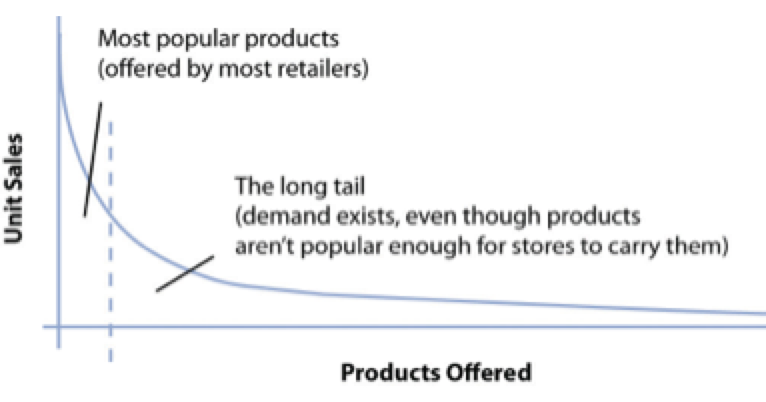
\includegraphics[width=0.75\textwidth]{long-tail.png}
    \caption{The long tail effect \cite{longtaileffect}}
    \label{fig:longtail}
\end{figure}

It especially was strengthened by the advent of Recommender Systems. By offering more personalised items to users, we can expose users to these hard-to-find items that would have been apparent in on a popularity list. Proof of the advantages Recommender Systems offer can be seen by the major companies that take advantage of these systems.


\subsubsection{Amazon} 
Amazon is a behemoth multi-billion dollar online retail company. According to Statista, in 2018, they generated 232.89 billion dollars \cite{statista}. In a 2013 article by Mckinsey \& Company, it is reported that 35\% of Amazon's revenue comes from its recommendation System. 

\subsubsection{Netflix}
Netflix is an online video streaming platform that offers thousands of TV Series and Movies to it's millions of users. Netflix uses a Recommender System not only to personalise the videos offered to the user, but also the artwork that is used as the thumbnail\footnote{a cover image for a video} for the video \cite{josefina2018netflix}.

These are just a few examples of platforms that benefit from Recommender systems \cite{polatidis2013recommender}.

\subsection{Machine Learning Approach} \label{subsec:mlApproach}
Machine Learning is a study of Artificial Intelligence that uses algorithms and models to enable computer systems learn how to perform tasks using data without the need for explicit instructions to be given \cite{michie1994machine}. Machine learning models are used for a variety of tasks such as classification\footnote{differentiation between items}, facial recognition, regression analysis and so on.

Regression Analysis is a set of techniques that discover relationships between variables in data \cite{chatterjee2015regression}. By trying to find a best fit between variables in data, you can discover the relationship between them and also predict values for new variables. Regression analysis can also be described as a predictive analysis, hence, Recommender Systems can be classified as a Regression Analysis problem, as the system try's to predict a user's predicted rating of an Item. Hence we have a means to creating a Recommender System using Machine learning Methods.

\section{GraphQL over REST}
Web applications consists of two main parts: the client, which contains the user interface the user interacts with, and the server, which provides the resources needed to be consumed by the client. In recent years, \acrfull{rest} has quickly been adopted in industry as the standard for creating a server \acrfull{api} \cite{guy2015rest}. They allow the client to access the resources provided in the server via stateless operations with the use of a \acrfull{url}. However one of the main problems with \acrshort{rest} is it's lack of flexibility. The resources in \acrshort{rest} are exposed via endpoints. The shape of the data returned to the client by theses endpoints are defined by the server. This can lead to problems of \gls{over-fetching} and \gls{under-fetching}. In \autoref{fig:restProblem}, we can see a standard \acrshort{rest} \acrshort{api} that exposes a users details, posts and followers via separate endpoints. The client is forced to make multiple requests to get the data required as each endpoint returns under-fetched. If the client requests only a users name from the user details endpoint, this leads to over-fetching of data.

\begin{figure}[htb!]
    \centering
    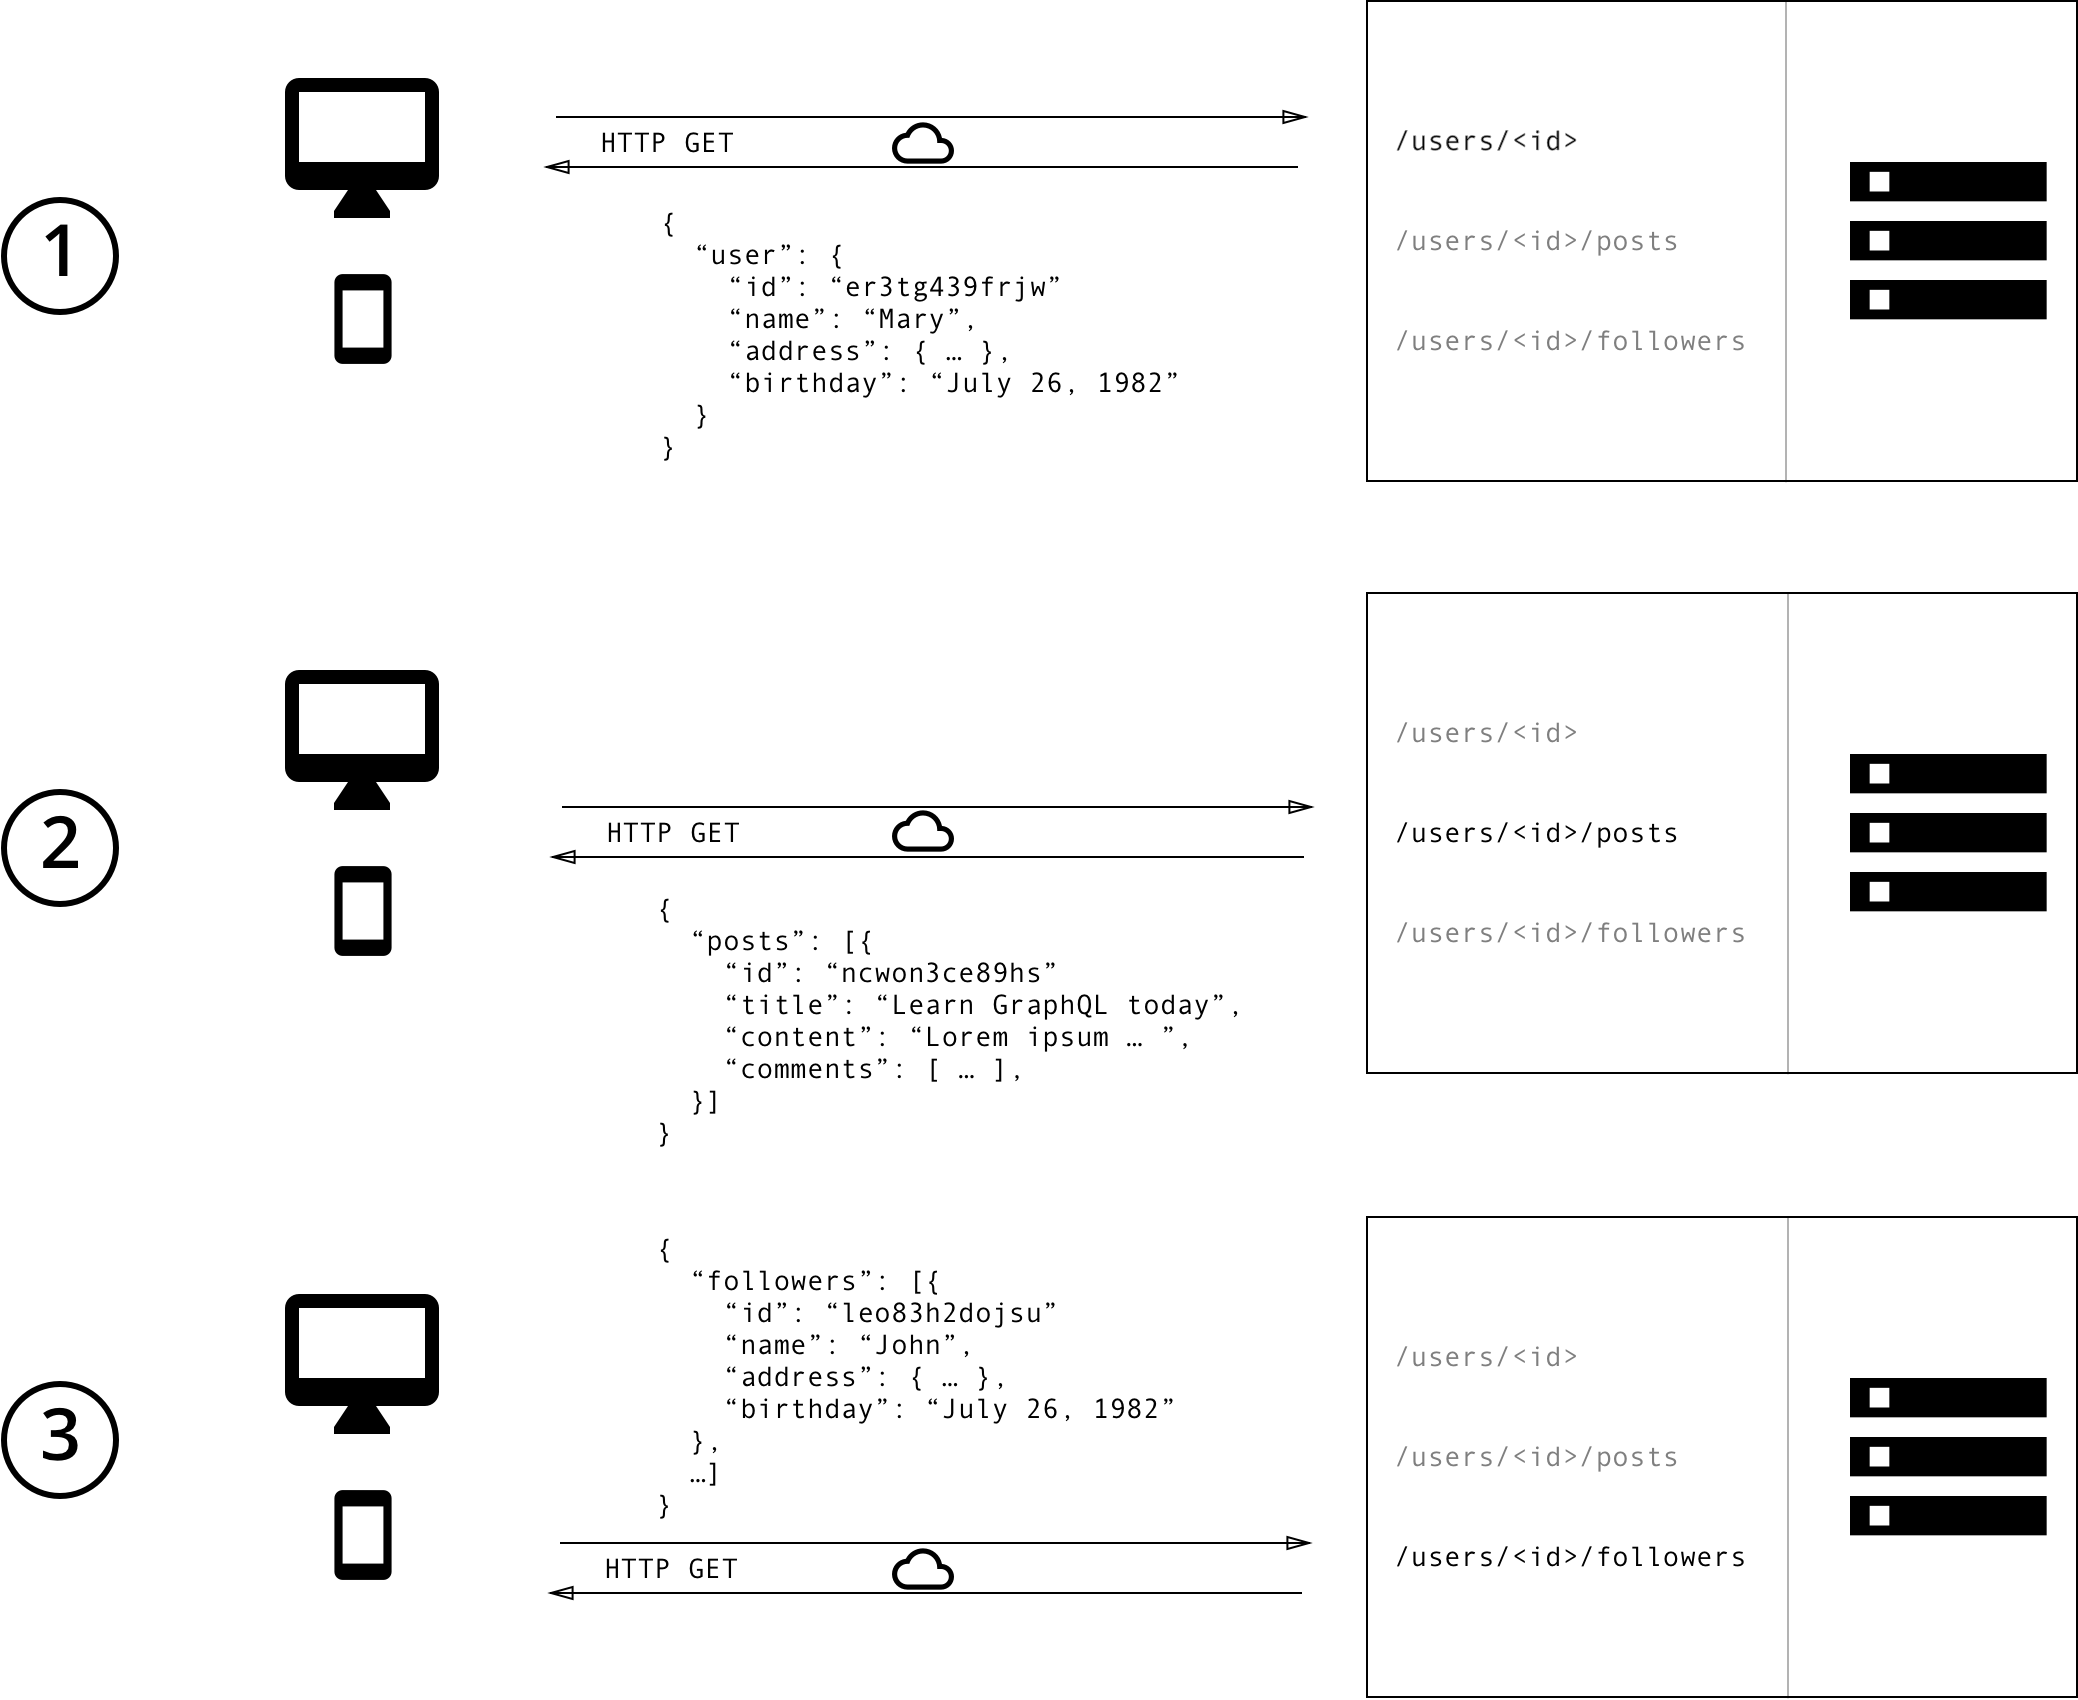
\includegraphics[width=0.75\textwidth]{problems-with-rest.png}
    \caption{REST having to make three separate requests to to three different endpoints to get the required data \cite{graphqlvsRest}}
    \label{fig:restProblem}
\end{figure}

GraphQL was introduced as a solution to the shortcomings with \acrshort{rest} GraphQL, created by Facebook in 2012, and then open sourced in 2015, is a query language for an \acrfull{api} and a run-time for fulfilling those queries with your existing data \cite{graphQl}.  Like \acrshort{rest}, GraphQL is used to expose resources to the client. However, GraphQl only exposes a single endpoint and the client defines the structure of the data that is required \cite{howToGraphQl}, eliminating the problem of over-fetching and over fetching. \autoref{fig:graphqlFix} shows how a GraphQL server can get the same data as the before, using only one request.

\begin{figure}[htb!]
    \centering
    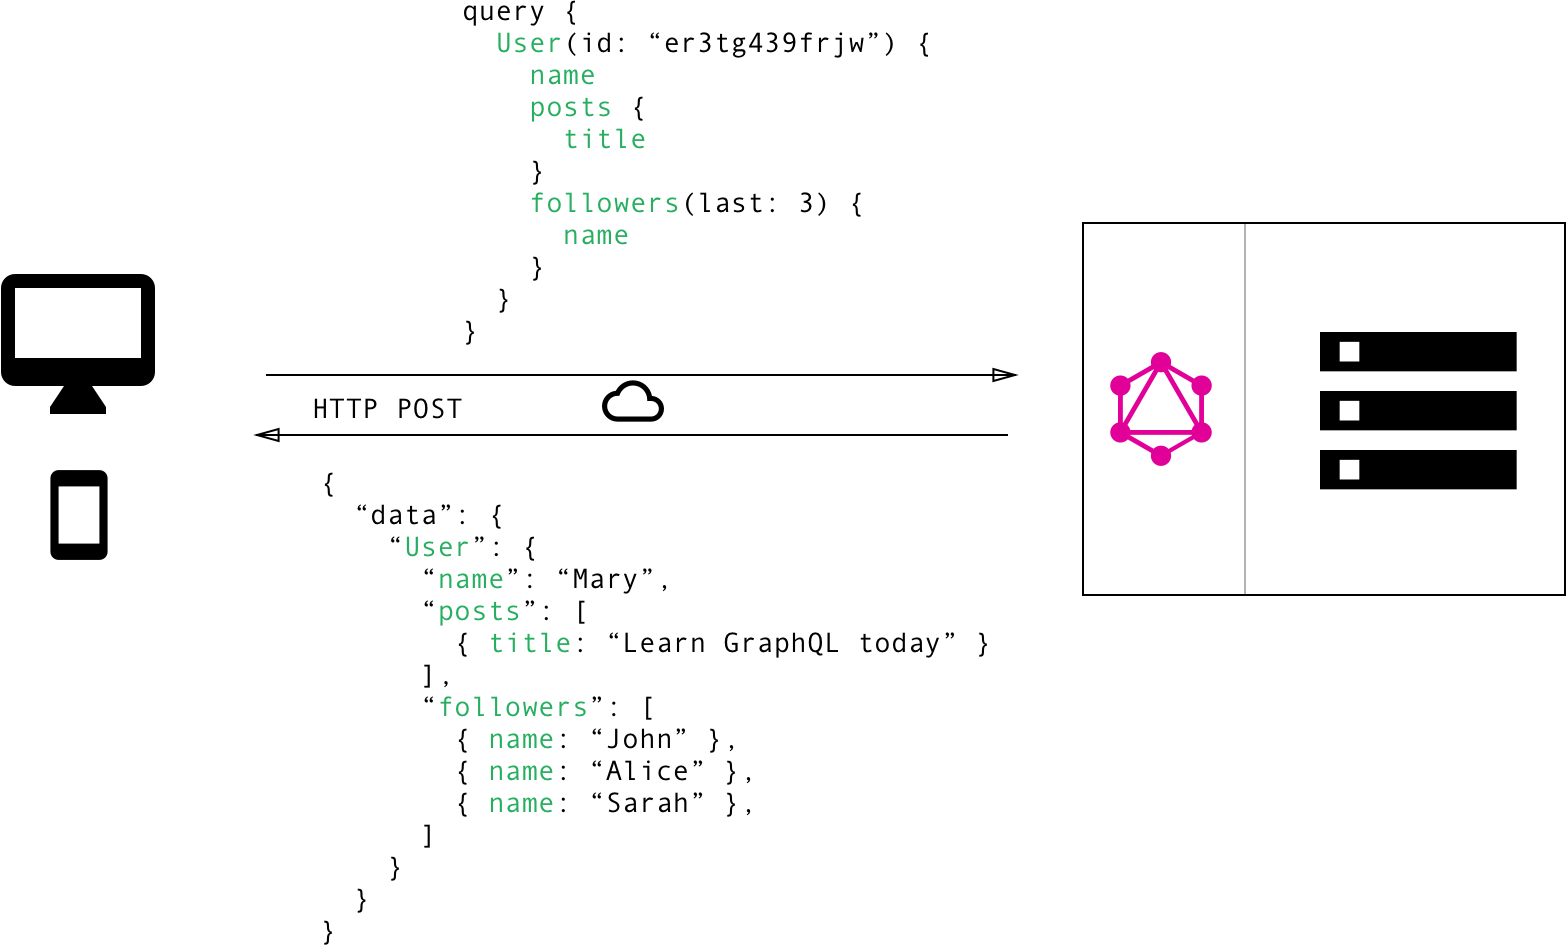
\includegraphics[width=0.75\textwidth]{fetching-graphql.png}
    \caption{GraphQl can perform retrieve the same required data using one request to one endpoint \cite{graphqlSolution}}
    \label{fig:graphqlFix}
\end{figure}

This is important in our application as in some scenarios where information is being retrieved, we would want to prevent over-fetching. To store trail information, a large number of coordinates per each trail needs to be stored. When a user is searching for a trail initially, only details such as the name of the trail, average rating and so on are required. Requesting all the coordinates would add unnecessary overhead to the system during communication between the client and server.
\chapter{An Interface For Trails} \label{chap:TrailInterface}
To facilitate the creation and exhibition of trails on a website, it is important to provide and interface that presents visual and contextual aid to the users as they are planning a path or exploring other paths. This chapter describes the two main methods used to provide such information via a Map Interface (discussed in section \ref{mappingPlatform}), and an Elevation Profile (discussed in section \ref{elevationProfile}. We discuss the decisions made and technologies used to provide these features.

\section{Mapping Platform Providers} \label{mappingPlatform}
The application provides an interactive map interface that users use to create trails. Trails are created by users clicking on points on the map. The system then calculates path between each two points created and connects to ensure that trails stay on the defined paths on the map.

To provide this, we need to use an open source map provider for the interface. In industry, there really three main providers: Google Maps, Mapbox and Ordinance Survey Maps. A comparison of these providers is shown in \autoref{tab:MappingPlatformsComparison} to help inform the decision on the chosen map provider.

To decide on what provider to use, I compare the benefits and negatives of all three in table \ref{tab:MappingPlatformsComparison}.

\begin{table}[htb!]
    \centering
    \begin{tabular}{lll}
        \hline
        \multicolumn{1}{c}{Map Provider} & \multicolumn{1}{c}{Advantages} & \multicolumn{1}{c}{Disadvantages} \\ 
        \hline
        \hline
        Google Maps & \begin{tabular}[c]{@{}l@{}}Very Accurate Map\\ Open Source Software\end{tabular} & Not very customisable \\
        \hline
        Mapbox & \begin{tabular}[c]{@{}l@{}}Open source software\\ Very customisable\\ Big community\\ Good documentation\end{tabular} & Relies on open sourced data \\
        \hline
        OS Maps & Maps are the most detailed & \begin{tabular}[c]{@{}l@{}}Not opened source\\ Only has UK map\end{tabular} \\ 
        \hline
    \end{tabular}
    \caption{Comparison of the different mapping providers that I could use}
    \label{tab:MappingPlatformsComparison}
\end{table}

Due to its big community and good documentation, Mapbox was the most suitable provider for this project. These reasons ensured development was a straightforward endeavour as there was a wealth of assistance available. Mapbox is also the map provider used by most of the example trail running applications discussed in \autoref{sec:TrailRunningApplications}, giving confidence by the fact that the provider has been tested and proven by other applications.


\subsection{Creating a Trail}
When a user clicks on the map, the system returns the coordinates of the point the user clicks on the map as shown in listing \ref{listing:exampleCoordinates}.

\begin{listing}[ht]
\caption{Example of coordinates returned from mapbox}
\inputminted[frame=lines,framesep=2mm,baselinestretch=1.2,fontsize=\footnotesize]{json}{listings/example-coordinates.json}
\label{listing:exampleCoordinates}
\end{listing}

We can use this data to draw points on the map interface, visually showing the points the user has clicked as shown in \autoref{fig:SinglePointCreated}.

\begin{figure}[ht]
    \centering
    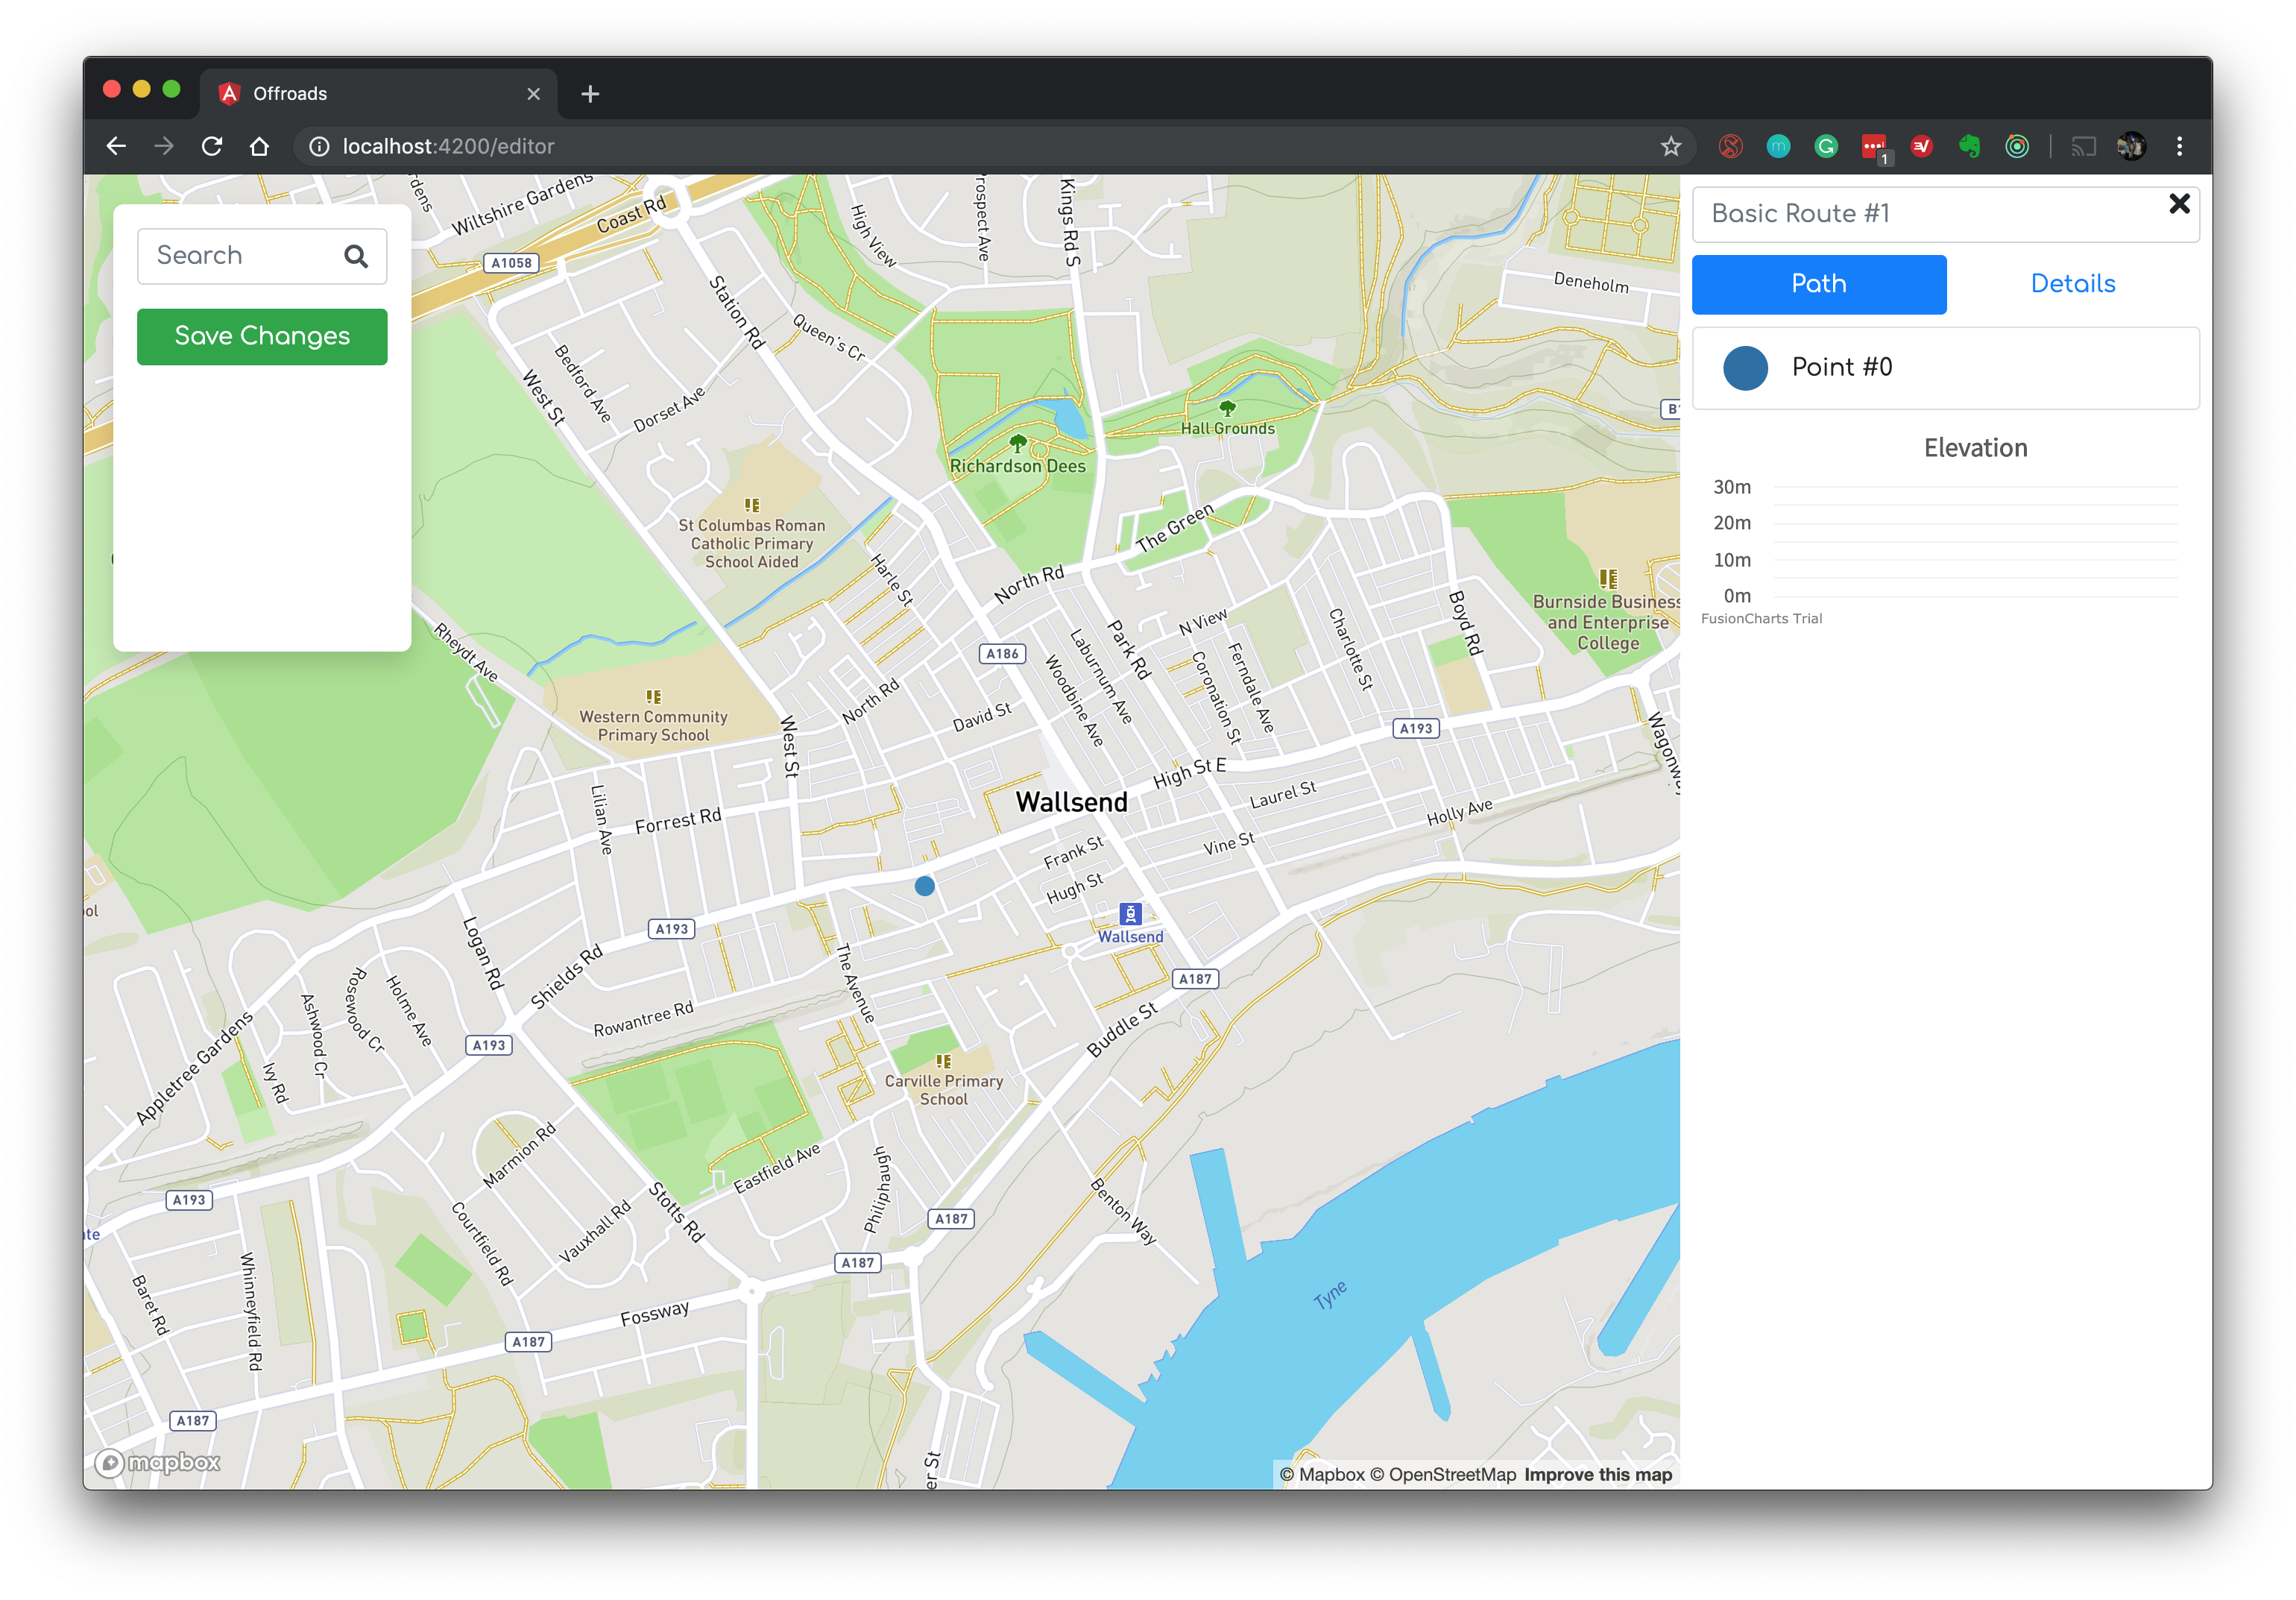
\includegraphics[width=0.75\textwidth]{single-point-on-map.png}
    \caption{The point created by a user clicking on the map indicating the location the user clicked in}
    \label{fig:SinglePointCreated}
\end{figure}
When the user adds an extra point, the system needs to combine these two points with a line. At this point, we need to calculate a path between the last point added and the new point that's just been added. When a user creates a path, it makes more sense for the path to follow already existing paths rather than a straight line that may cross over paths and terrains. Hence we need to calculate a path from between the two points to draw the line. Mapbox provides a Directions \acrshort{api} to help us do this.


\subsubsection{Finding a path}
Mapbox's Direction \acrshort{api} allows us to find a path between two points by querying the \acrshort{api} with a \textit{start} and \textit{end} coordinates.  The \acrshort{api} then returns us a a \acrshort{json} object describing the path between the specified starts and end points and the distance between the two points specified (an example is shown in appendix \ref{appSec:mapboxDirections}). We we use this data to draw a line between the two points that will follow the path returned (see figure \ref{fig:PathCreated}).

\begin{figure}[htb!]
    \centering
    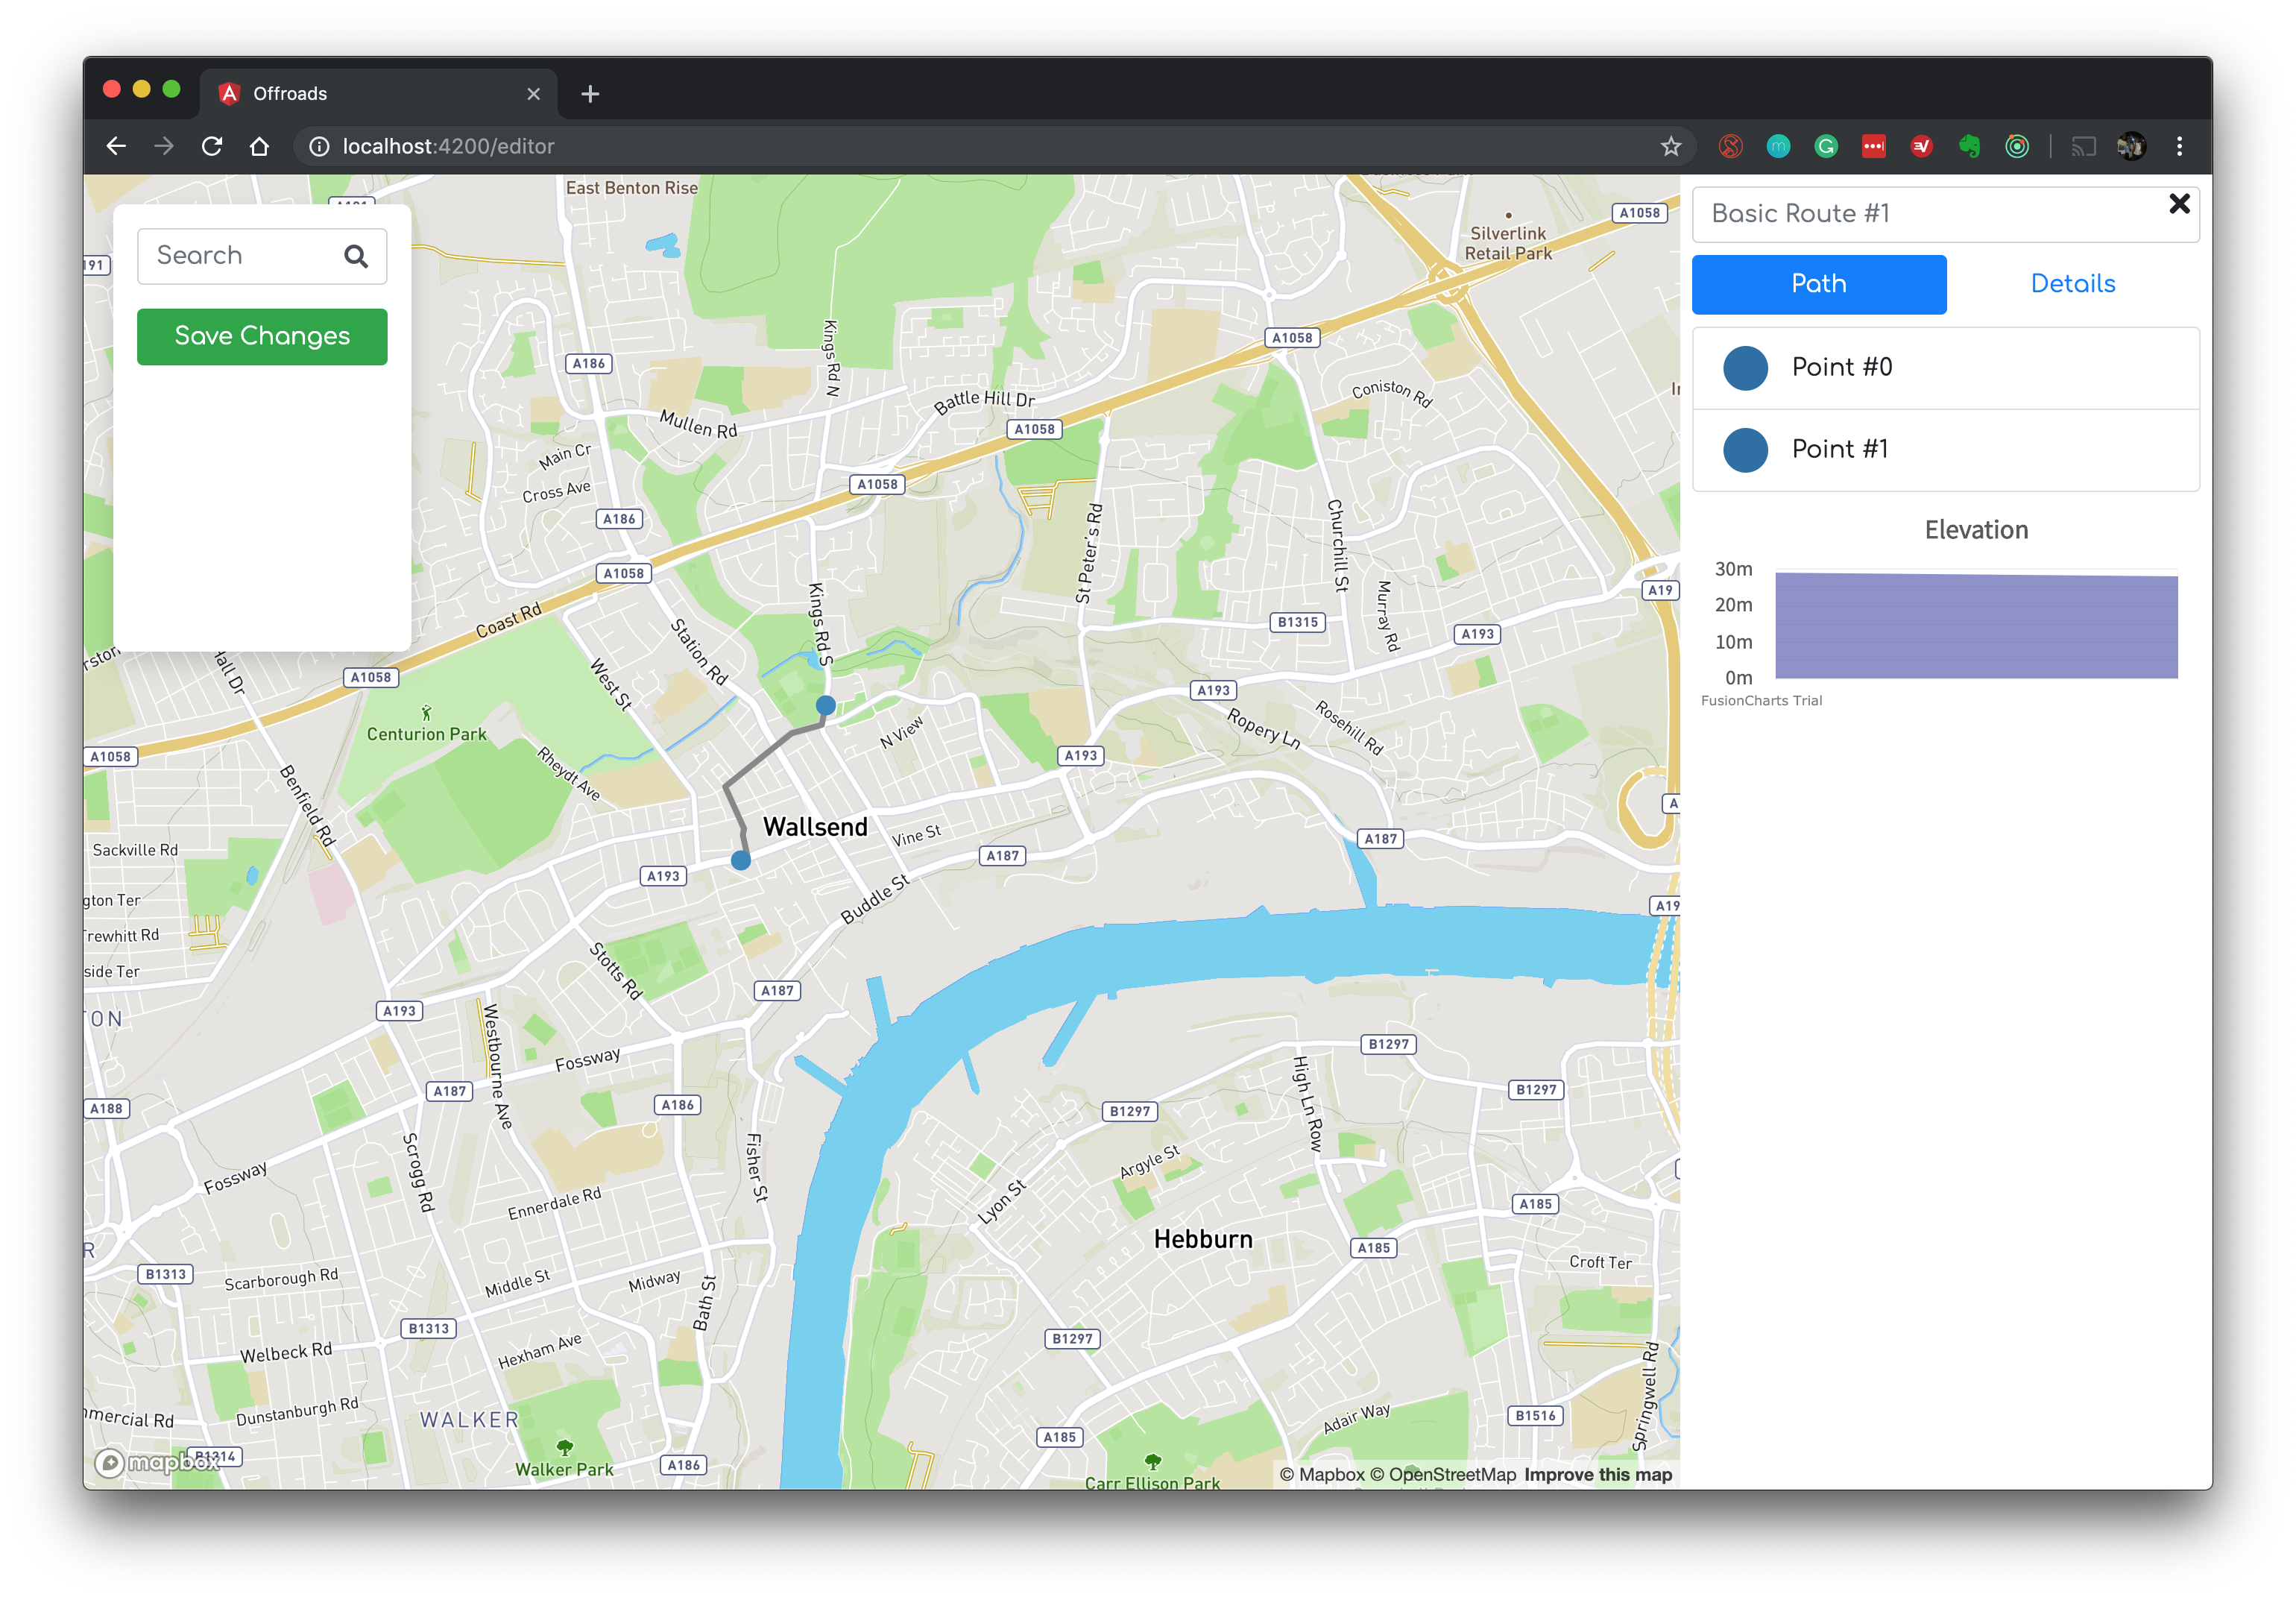
\includegraphics[width=0.75\textwidth]{path-between-points.png}
    \caption{Path created from the directions returned by the Mapbox API}
    \label{fig:PathCreated}
\end{figure}

\section{Presenting Elevation Profiles} \label{elevationProfile}
Trail runner's often use the elevation of a trail to help decide the type of trail that they wish to run. For this, the map interface provides contours that allow users to anticipate the steepness of the trail that they are creating or that they wish to run as shown in figure \ref{fig:MapContours}.

\begin{figure}[htb!]
    \centering
    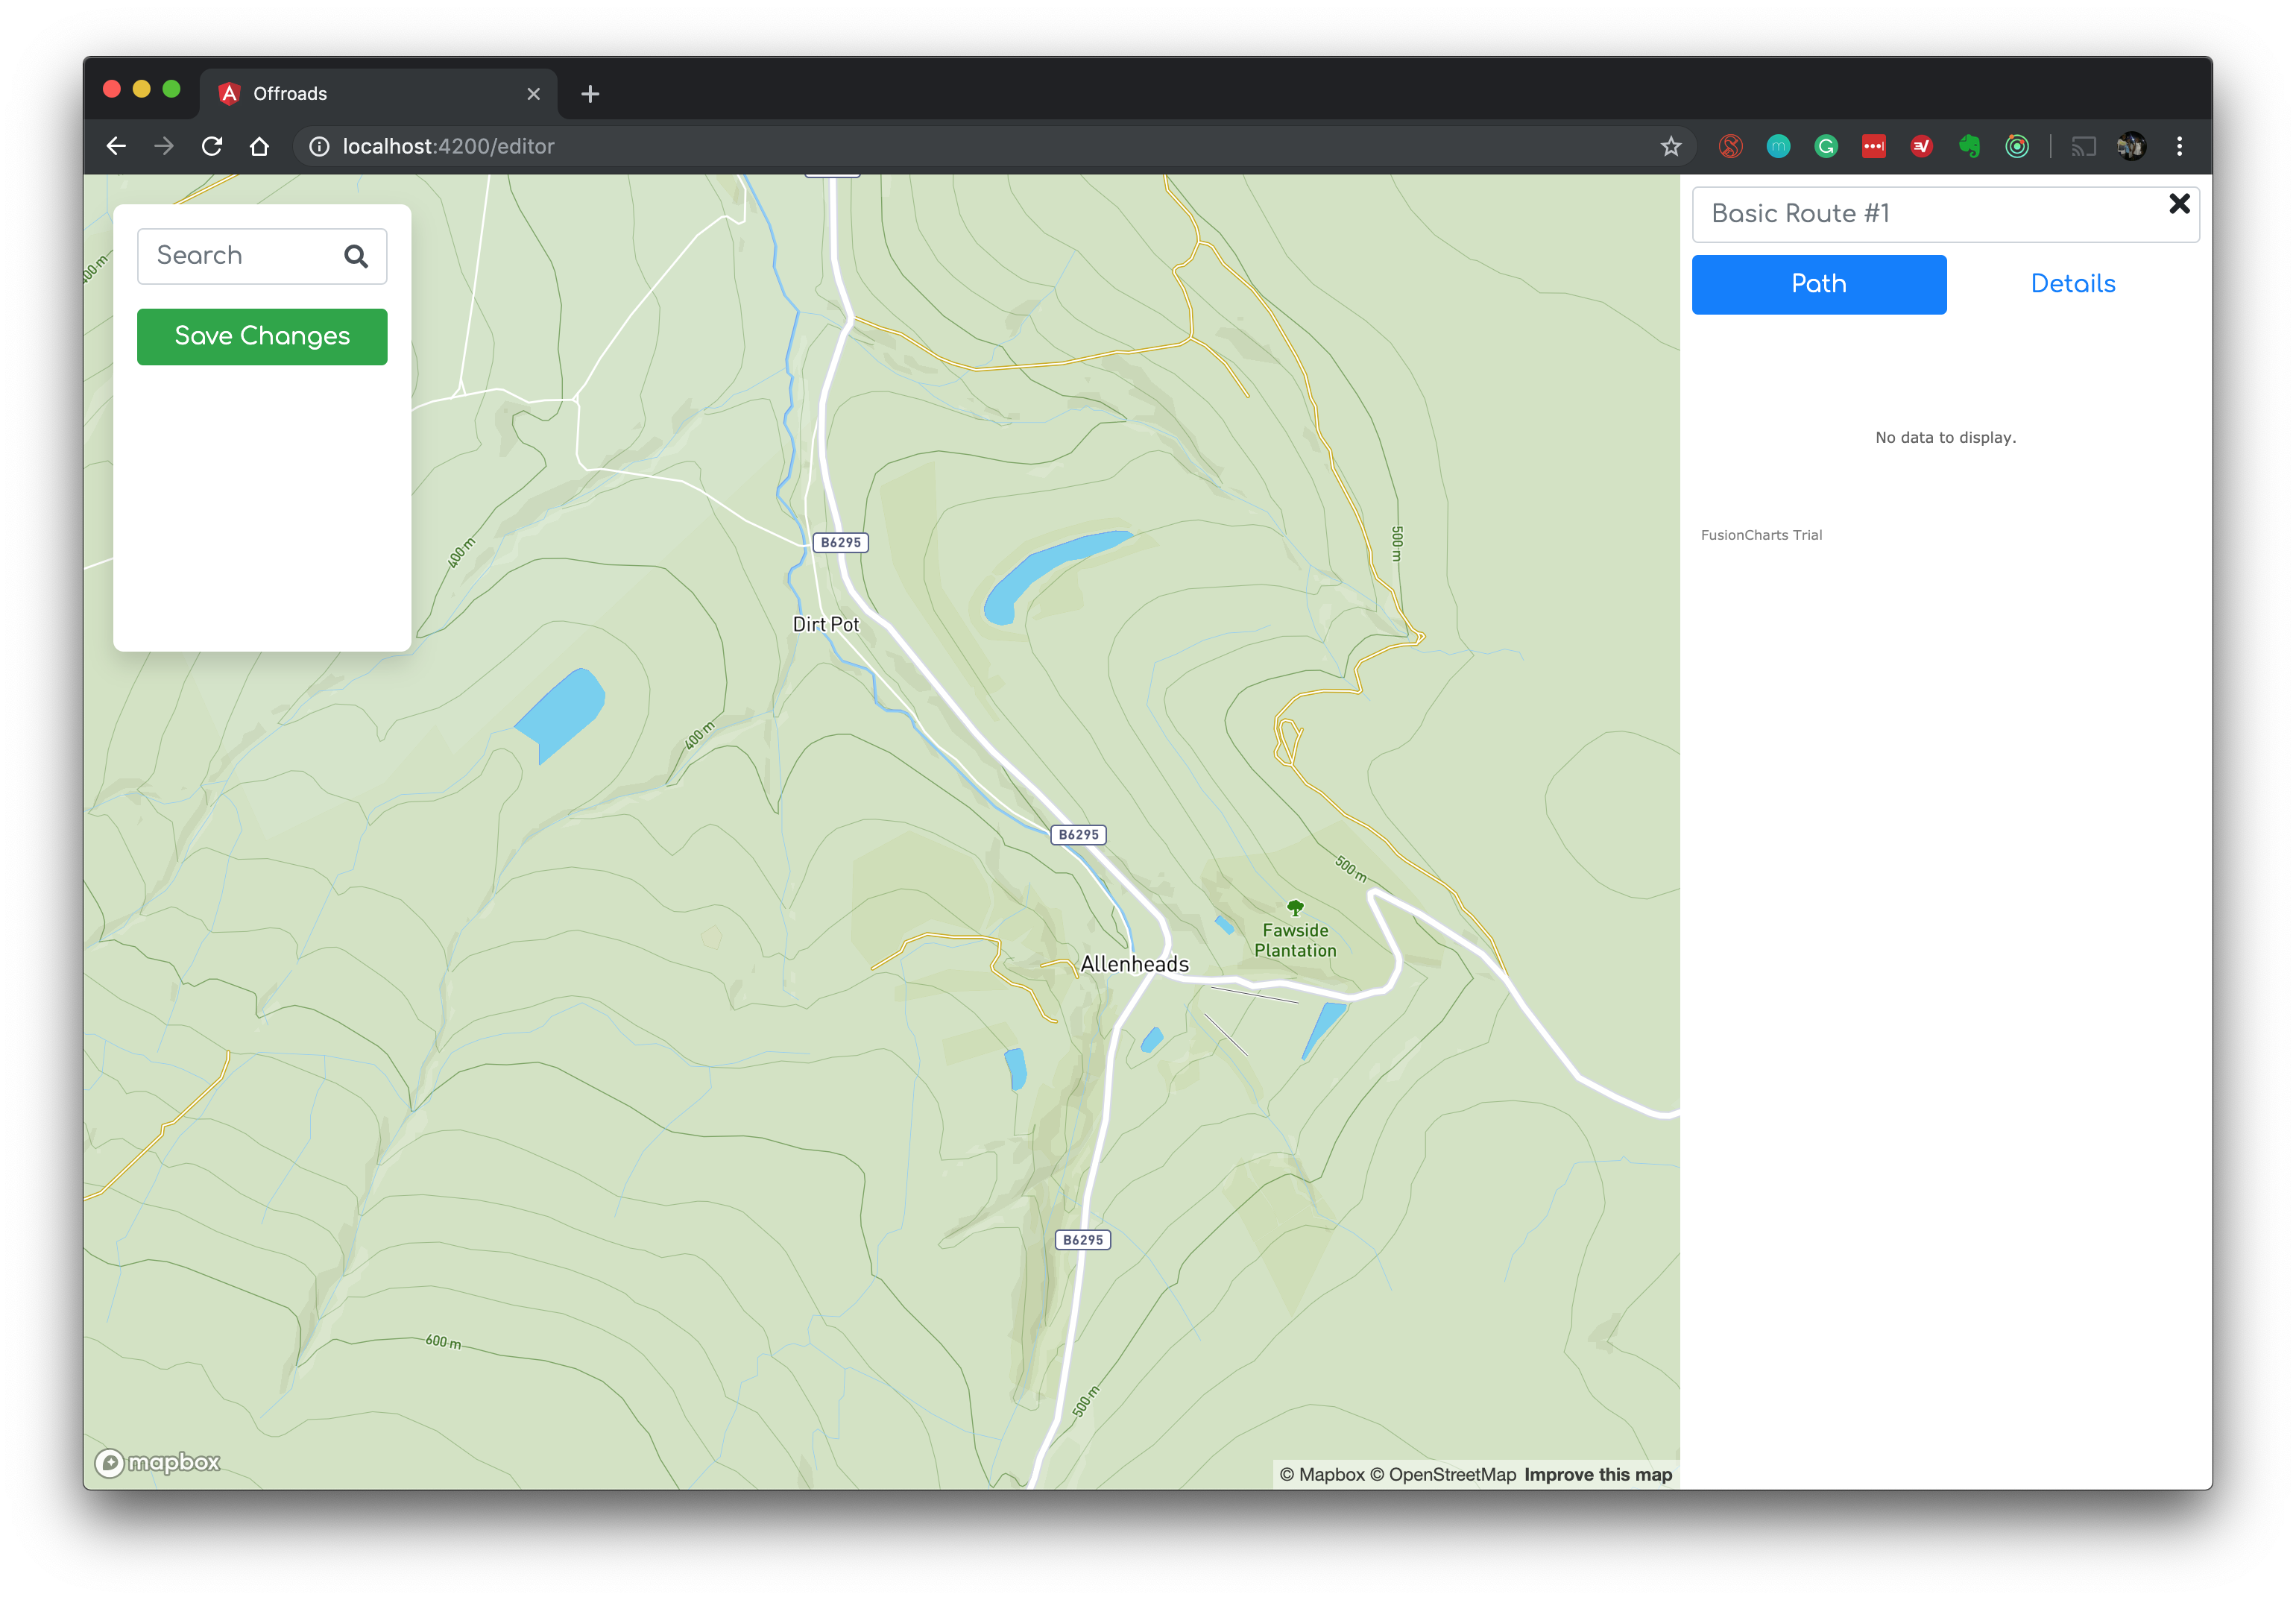
\includegraphics[width=0.75\textwidth]{map-contours.png}
    \caption{Contours on the map to help find elevation}
    \label{fig:MapContours}
\end{figure}


However, for the uninformed, reading contours can prove to be an unusual task. A better way of representing the elevation profile of is via a Graph. This will allow the user to view the elevation of a route against the distance of the route, giving a more detailed view of the elevation of the trail.

The Mapbox Directions API only provides an elevation of specific way-points of the path that is returned as shown in appendix \ref{appSec:mapboxDirections}. Although this provides some elevation information, it is not sufficient enough as the elevation of a trail can change drastically withing way-points.

Google offers an elevation service that allows you to query a trail and returns a detailed elevation profile of that trail as shown in appendix \ref{appSec:googleElevation}. As a trail is being created, we send another request to the Google elevations service to get this information. We then plot on the graph the line the line that is returned, updating it as we trail is updated. The graphing \acrshort{api} that we use is Fusion Charts \cite{fusionCharts}.
\chapter{Architecture} \label{chap:Architecture}
To build Offroads, many technologies needed to be harnessed in order to produce the features needed for the Trail Running Website. In \autoref{chap:TrailInterface} we discussed the interface used to create and display trails, in this chapter we discuss how we provide this interface to the user with our chosen \Gls{front-end} framework in \autoref{sec:frontendFramework}. We discuss the extra features needed that the web application provides in \autoref{sec:ExtraFeatures}.

\section{Overview}
The client of the web application (including the trail interface described in chapter \ref{chap:TrailInterface}) are created with Angular. The client sends to and retrieves data from a GraphQl Server. The GraphQl Server is connected to a MySQl database. Prisma provides a GraphQl \acrfull{dal} to simplify to the database. This overall structure can be seen in \autoref{fig:graphArchitecture}. Our server responds with data written in \acrfull{json} format.


\begin{figure}[htb!]
    \centering
    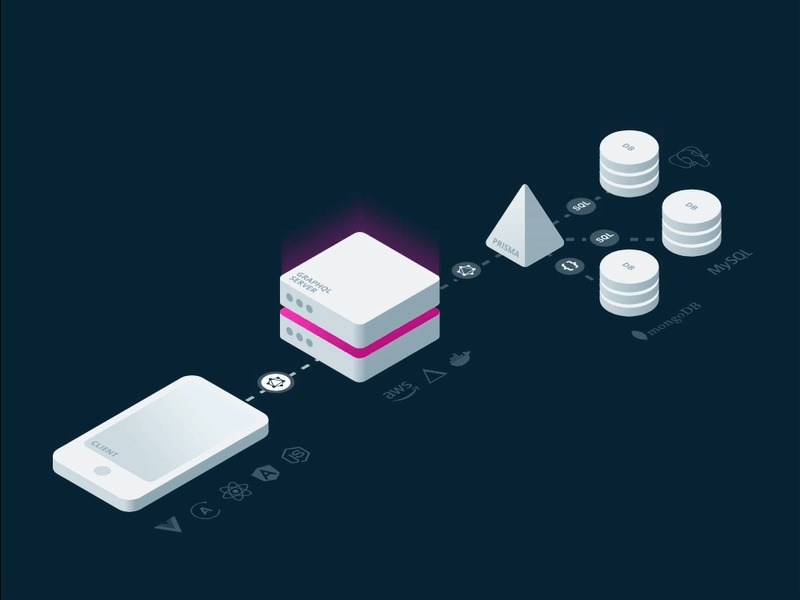
\includegraphics[width=0.75\textwidth]{graphql-architecture.jpg}
    \caption{Overall Architecture of the web application \cite{graphqlStructure}}
    \label{fig:graphArchitecture}
\end{figure}


\section{GraphQL Backend}
To enable GraphQL on the \gls{back-end}, a GraphQ; schema has to be defined. This schema describes the type of data that can be returned and the operations that can be performed by the GraphQL server (see Appendix \ref{appsec:servergraphql}). A GraphQL Server supports 3 main operations:

\begin{itemize}
    \item Queries: reading data (analogous to GET requests from \acrshort{rest})
    \item Mutations: modifying data (analogous to POST and PUT request from \acrshort{rest}), and,
    \item Subscriptions: subscribing to real-time changes to data.
\end{itemize}

Whenever the client sends any of the above operations, the client also defines the shape of the data it wants to be returned. This then has to be parsed by the GraphQL who uses resolver functions to retrieve the data the client requests for and stitches them in the shape requested. This allows for a GraphQl server to have multiple data sources.

\subsection{GraphQL resolver functions}
GraphQL executes the query in the shape \cite{jonas2016graphql}. It first executes the root query and then traverses down the tree of the structure defined by the user, calling all the resolver functions needed to return the data required (see \autoref{fig:graphQlResolver}.


\begin{figure}[htb!]
    \centering
    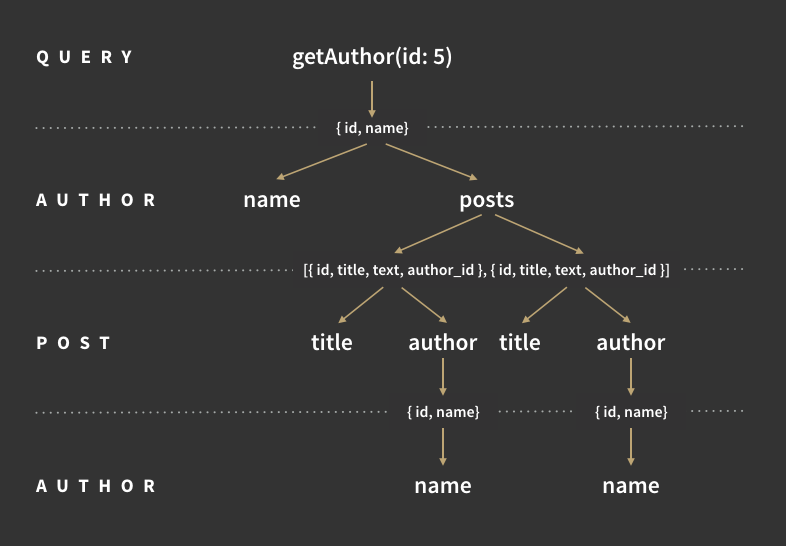
\includegraphics[width=0.75\textwidth]{graphql-resolver.png}
    \caption{GraphQL resolver function broken down in execution order \cite{jonas2016graphql}}
    \label{fig:graphQlResolver}
\end{figure}

This benefit to the client comes with its own complexities. As we use an SQL database, having to write queries for each resolver function that needs to be called can become counter intuitive to the advantages provided. This is why we use Prisma as a \acrfull{dal} between our server and our database.

\subsection{Prisma Layer}
Prisma \cite{prisma} is a data access layer that replaces traditional \acrfull{orm}. It sits in front of databases and provides methods that allow the server to access the database. The main feature that it provides is the Prisma Client, which is an auto-generated type-safe database client that creates the data access layer. Rather than having to write the SQL queries, Prisma reads our GraphQL schema and uses that to generate functions we can use to access our database (see \autoref{fig:prismaGenerate}).

\begin{figure}[htb!]
    \centering
    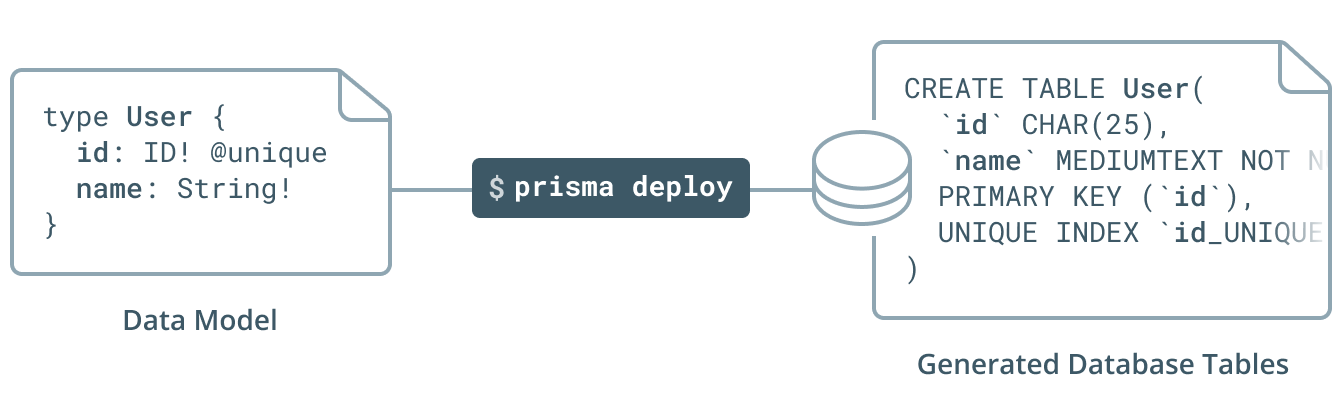
\includegraphics[width=\textwidth]{prisma-generate.png}
    \caption{SQL query generated from graphQL datamodel \cite{prismageneratesql}}
    \label{fig:prismaGenerate}
\end{figure}


\section{Frontend Framework} \label{sec:frontendFramework}
There are 2 main ways to build modern web applications. It can be done using native web stack of HTML, CSS and JavaScript or (and more popularly), built using modern web application frameworks. Although there are many proponents to building with the native web stack, modern applications, such as this one, are more complex in nature and hence, require tools make it easier to build complex solutions. They also have big communities and strong documentation that make debugging easier \cite{medium:WhyModernJSFrameworkExist}.

There are a large variety Frontend Frameworks out there. I considered the most popular ones which where
\begin{itemize}
    \item Angular \cite{angular}
    \item React \cite{react}
    \item Vue.js \cite{vuejs}
\end{itemize}

The framework I decided on was Angular. This was because it has excellent and well-detailed documentation, it came out of the bag with all most of the tools I needed to get started with, and it used Typescript over JavaScript.

\subsection{State Management With Redux}
One of the main problems that comes with building web applications is managing state in the \gls{front-end}. On the editor page, where user's create and trails, It is important to manage the state of the application to allow users to undo and redo any changes they make when creating or editing Trails.

Redux is JavaScript library created by Facebook use for managing state in user interfaces \cite{wiki:Redux}. NgRx \cite{cheng2018state} is a framework built on the fundamentals of Redux\footnote{The Flux Architecture}, to enable us to maintain state in our Application. It is provides a functional way of building Reactive Applications.

With NgRx we can easily manage and control the state of our web application. This is especially useful in on the editor page, where users can create trails described in \autoref{chap:TrailInterface}. NgRx helps us manage the state tree (shown in \autoref{fig:reduxStateTree}) of our application in the form of a stack, including the actions users use to create trails. This allows us to traverse the stack of the users actions allowing for redoing and undoing.

\begin{figure}[htb!]
    \centering
    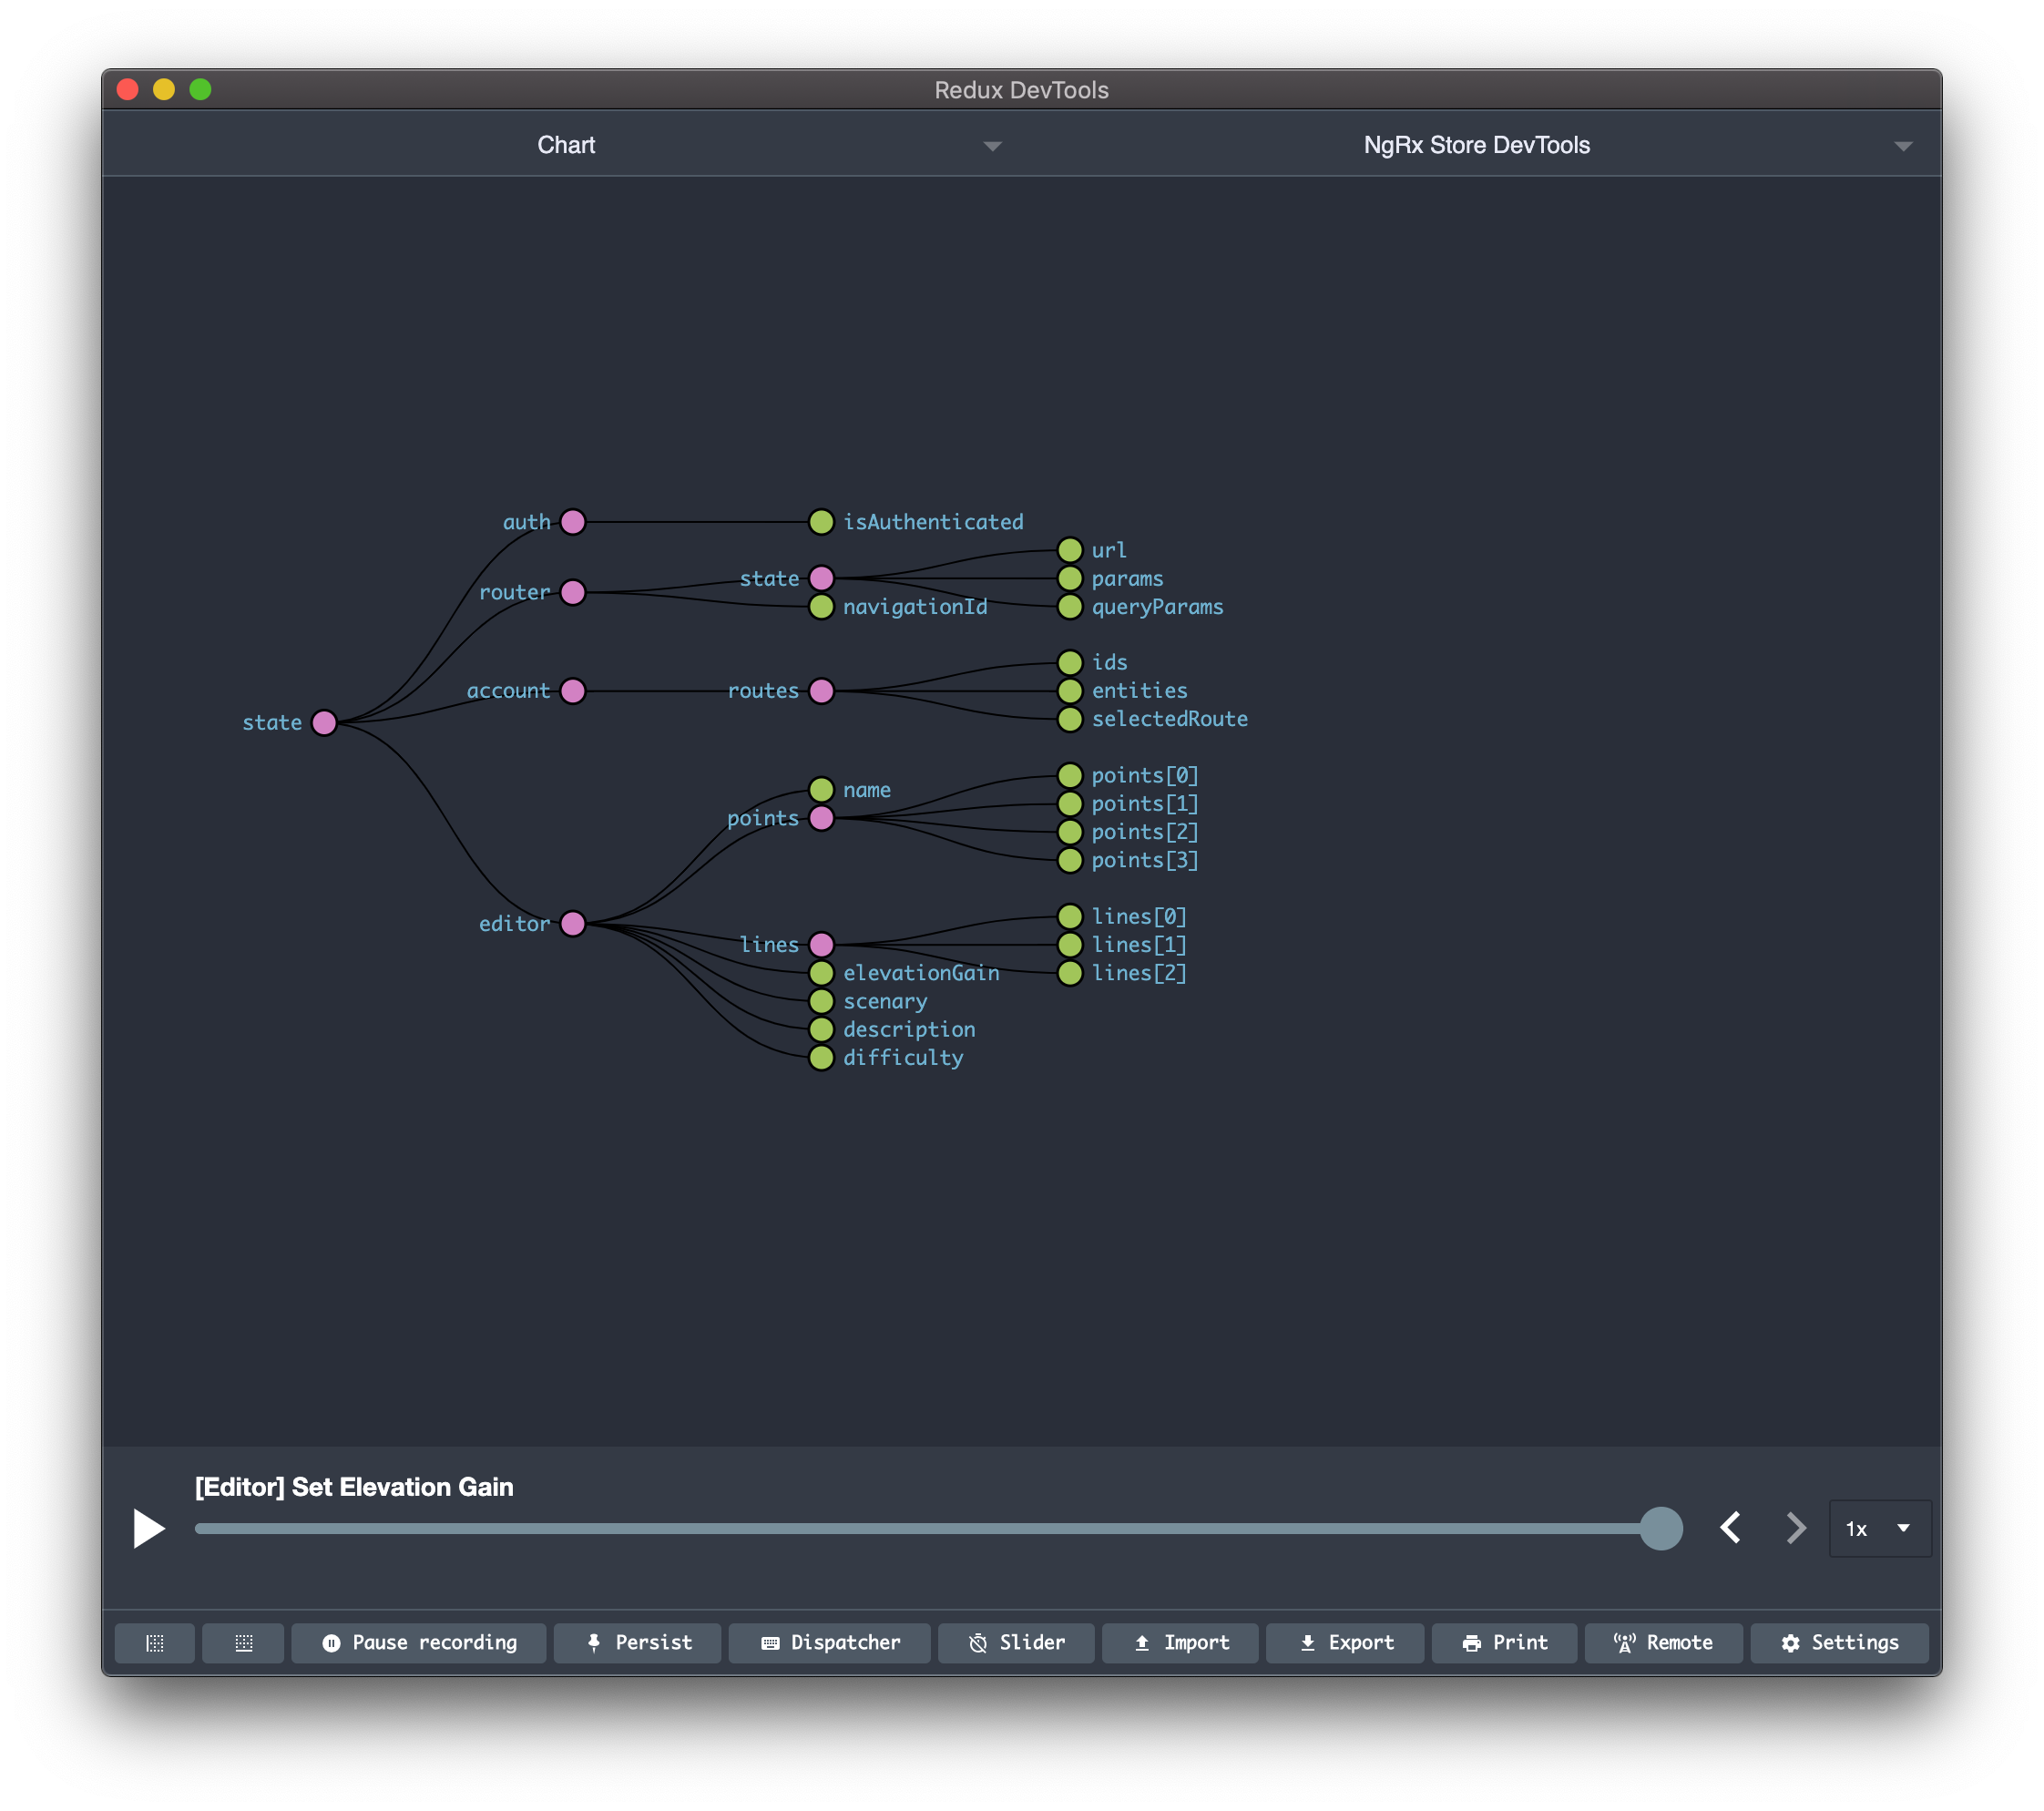
\includegraphics[width=0.75\textwidth]{ngrx-state-tree.png}
    \caption{Redux State tree show of the current state of the application}
    \label{fig:reduxStateTree}
\end{figure}

\section{Authentication and Authorisation}
\Gls{authentication} and \gls{authorisation}  are a crucial part of Identification any web application s to ensure the users can only interact data intended for them. Moreover, it is needed to allow users to be able to log-in to the system. The system provides authentication and authorisation with the power of \acrfull{jwt}.

\acrshort{jwt} is a compact open standard (RFC 7519), that allows the secure transmission of tokens between two parties in  \acrshort{json} format \cite{jones2015json}. The information shared between the two parties is digitally signed, and hence can trusted between be verified and trusted by the parties \cite{auth02019json}. This gives us a lightweight way of providing authentication and authorisation between the client on our user and the server.

Each user has a unique email they add when they sign-up as defined in our schema. When a user, attempts to log in with their email (which is unique to each user) we find the user in the database and their user ID. Once the Id is found we digitally sign the user ID using the standard with secret. The system uses the standard \acrfull{hs256} algorithm which is a combination of a \acrlong{hmac} and \acrlong{sha-256}.This token is then sent the the client and the client can store this token locally.

Whenever the client needs to authorise themselves, the client sends the request information (such as a query) and the token as part of the Authorisation header. The server reads the token from the header and can use that to verify client, granting them authorisation when needed.

\section{Necessary CRUD operations} \label{sec:ExtraFeatures}
\acrfull{crud} are the four basic operations that most web applications need to provide \cite{codeacademy2019crud}. They are self explanatory verbs that provide the essential operations user's need to be able to interact with web applications. The system provides a few \acrshort{crud} operations, enabling the user to access and manage their data.

\subsection{Uploading a Trail}
When a user creates a trail using the map interface described in \autoref{chap:TrailInterface}, it is persisted to the server to be stored in the database. The information needed to be stored for trails are the name of the trail (for identification and searching), points and the lines (made up of coordinates) that are used to create the trail. We store the points and lines to be used to redraw the trail on the map interface when presenting it to the user. A user can have multiple created trails

\subsection{Exploring Trails}
Exploring trails is how users can find new trails. The main way users can explore trails is via the Recommender system discussed in \autoref{chap:Recommender}. The system also provides other methods to allow users to find trails.

\subsubsection{Sorted Ranked List of Trails}
On the main explore page, there are tabs displaying trails in sorted ranked list. Although in \autoref{subsec:WhyRecSystems}, we discuss the importance of using Recommender systems to suggest trails, the Recommender system is slightly ineffective with new users who are yet to run a trail. Hence we provided other methods of ranking trails to the user.

\begin{itemize}
    \item \textbf{Popular trails:} Trails sorted in descending order of the number of users who run the trail (i.e. trails with the most runs are ranked at the top). 
    \item \textbf{Top rated trails:} Trails sorted in descending order of the average rating from users who run the trail.
    \item \textbf{Recently added trails:} Trails sorted in descending order of the date they where created.
\end{itemize}

\begin{figure}[htb!]
    \centering
    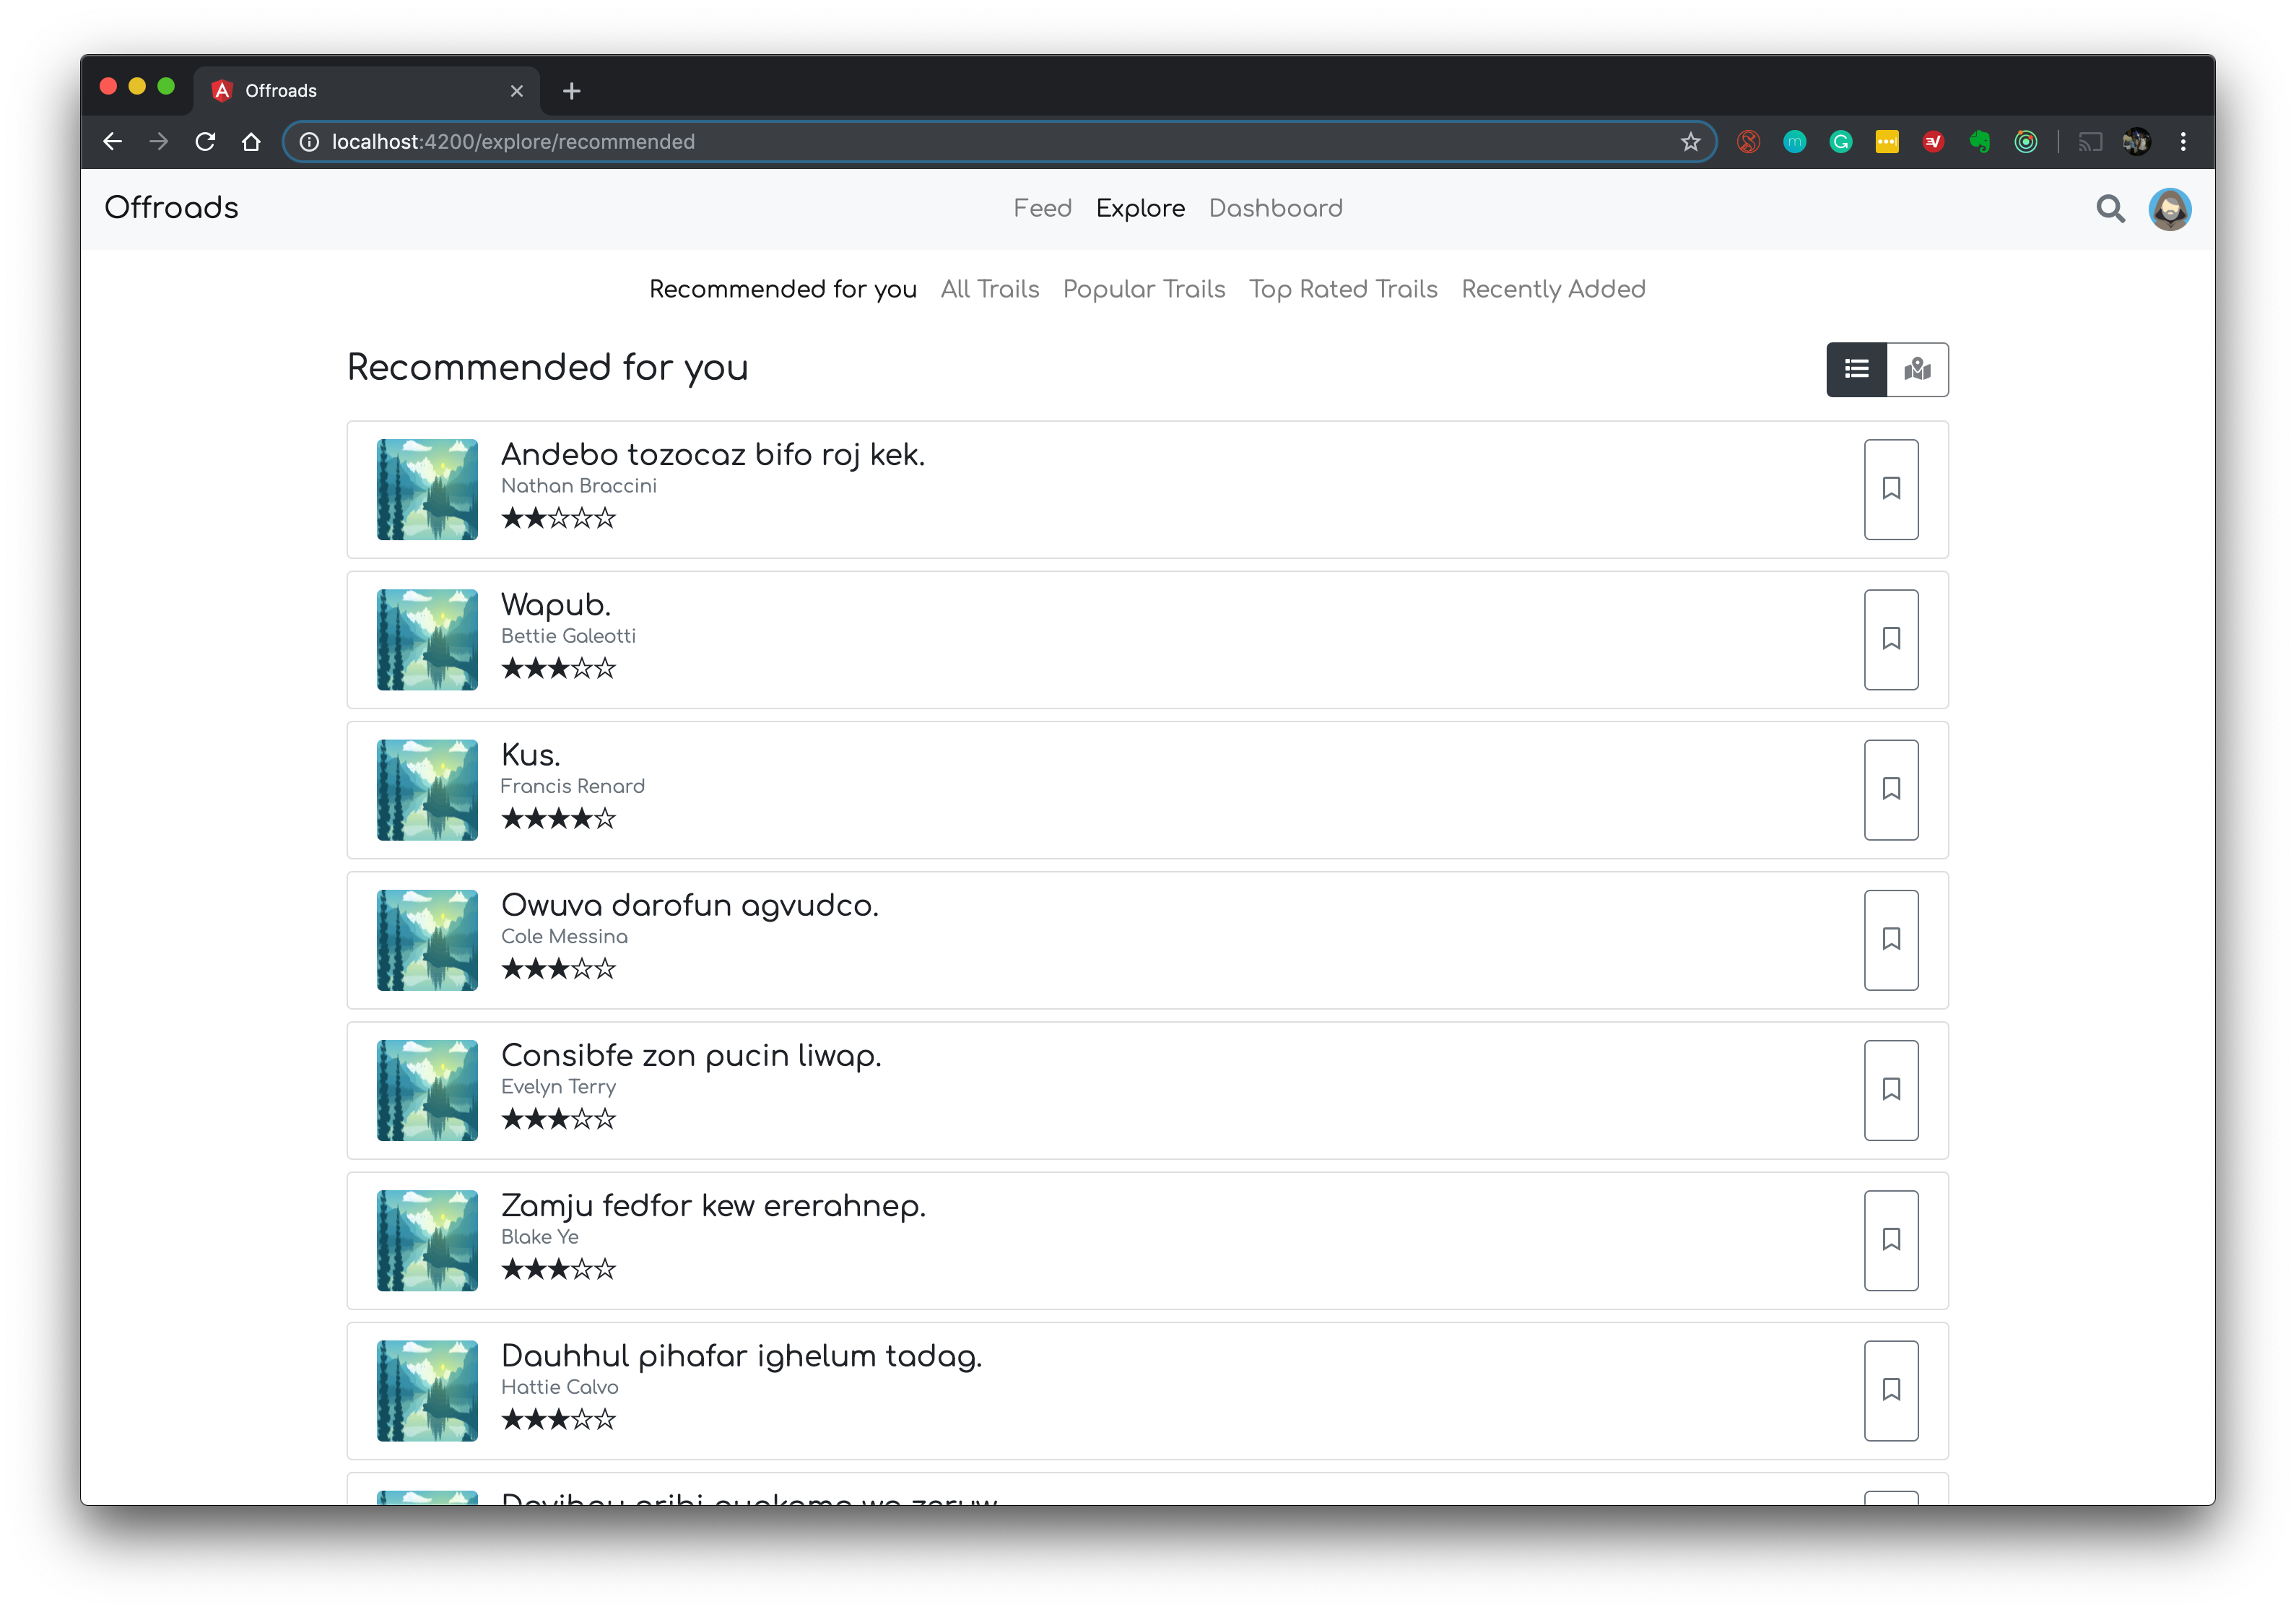
\includegraphics[width=0.75\textwidth]{explore-page.png}
    \caption{Explore page with tabs of all the different forms of rankings}
    \label{fig:explorePage}
\end{figure}

\subsubsection{Real time Search}
The system offers the capability of real time searches of trails and users by name using Regular Expression. To do this, they server will need to be queried as the user types in the search string, creating a performance bottleneck. Angular comes built in with a technology called RxJs that allows us to alleviate this bottleneck. By debouncing the requests such, that it is not on every keystroke, we can improve the performance.

\begin{figure}[htb!]
    \centering
    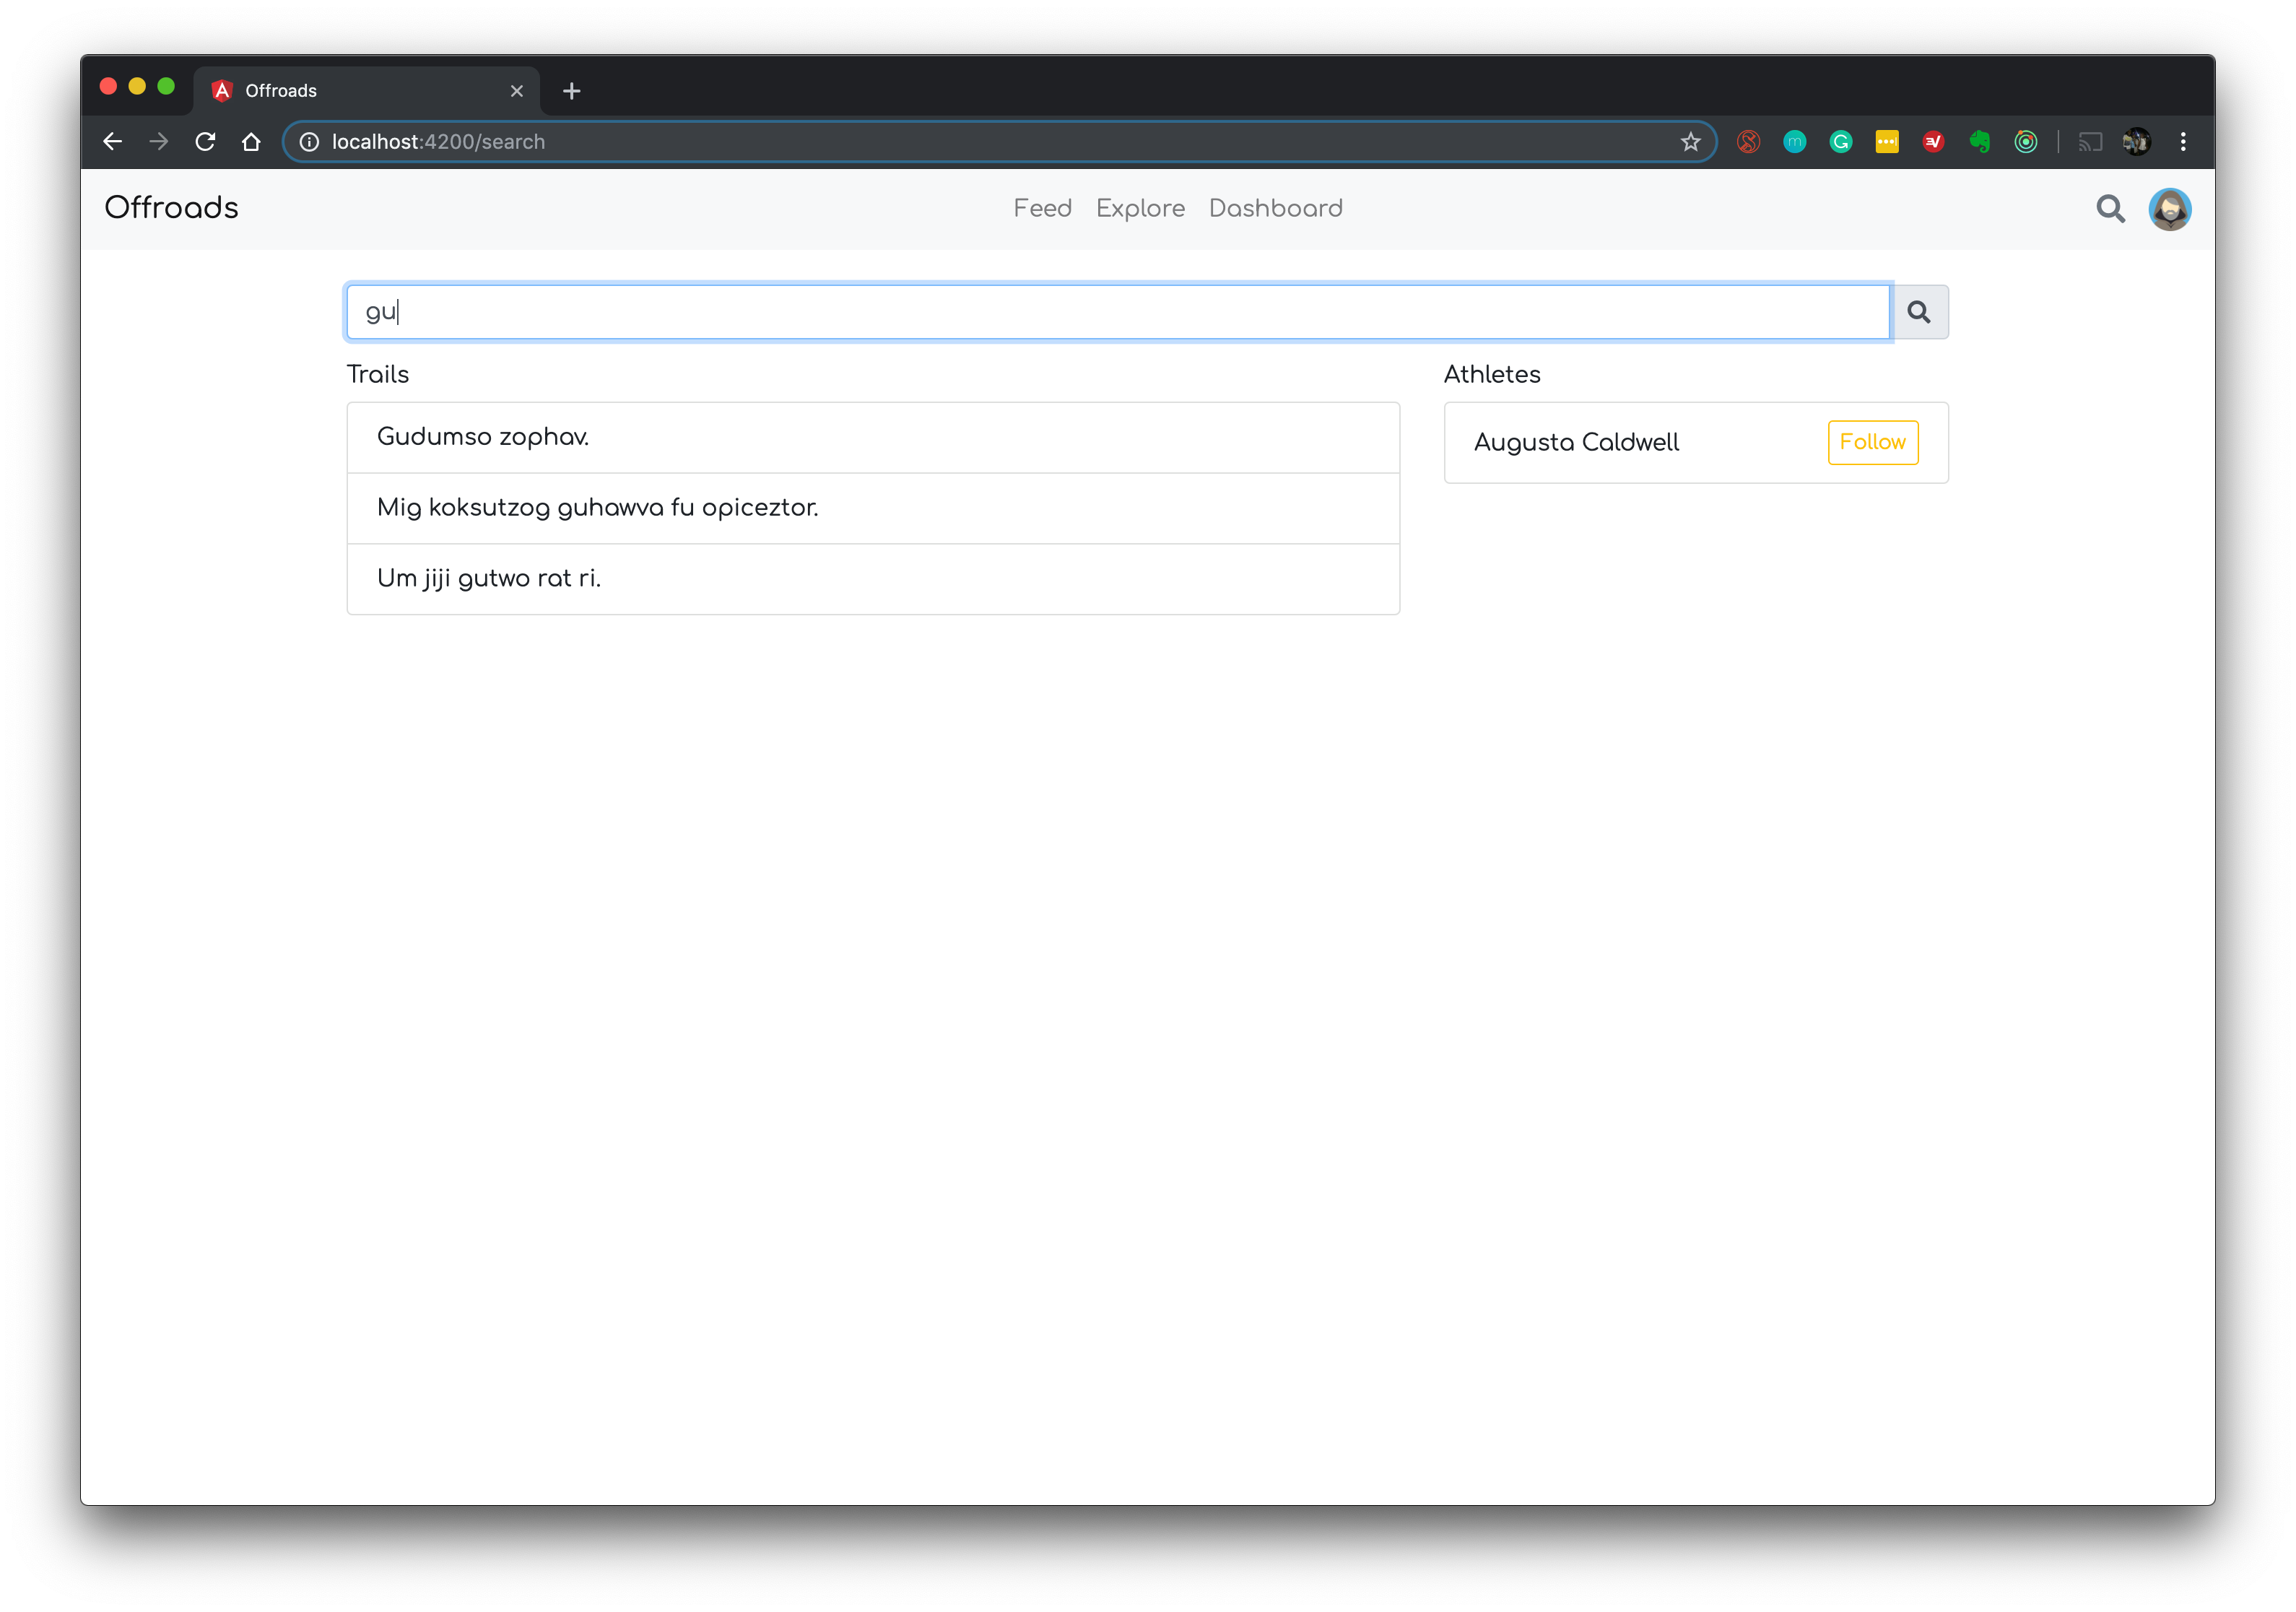
\includegraphics[width=0.75\textwidth]{search-page.png}
    \caption{Search page with the results of search}
    \label{fig:searchPage}
\end{figure}


\subsection{Trail Description Page} \label{subsec:trailDescription}
The trail description page includes all the information about a trail. It includes details such as the name of the trail, average rating of the trail and so on (an example is given in \autoref{fig:trailDescriptionPage}) and also includes the trail itself and elevation profile

\begin{figure}[htb!]
    \centering
    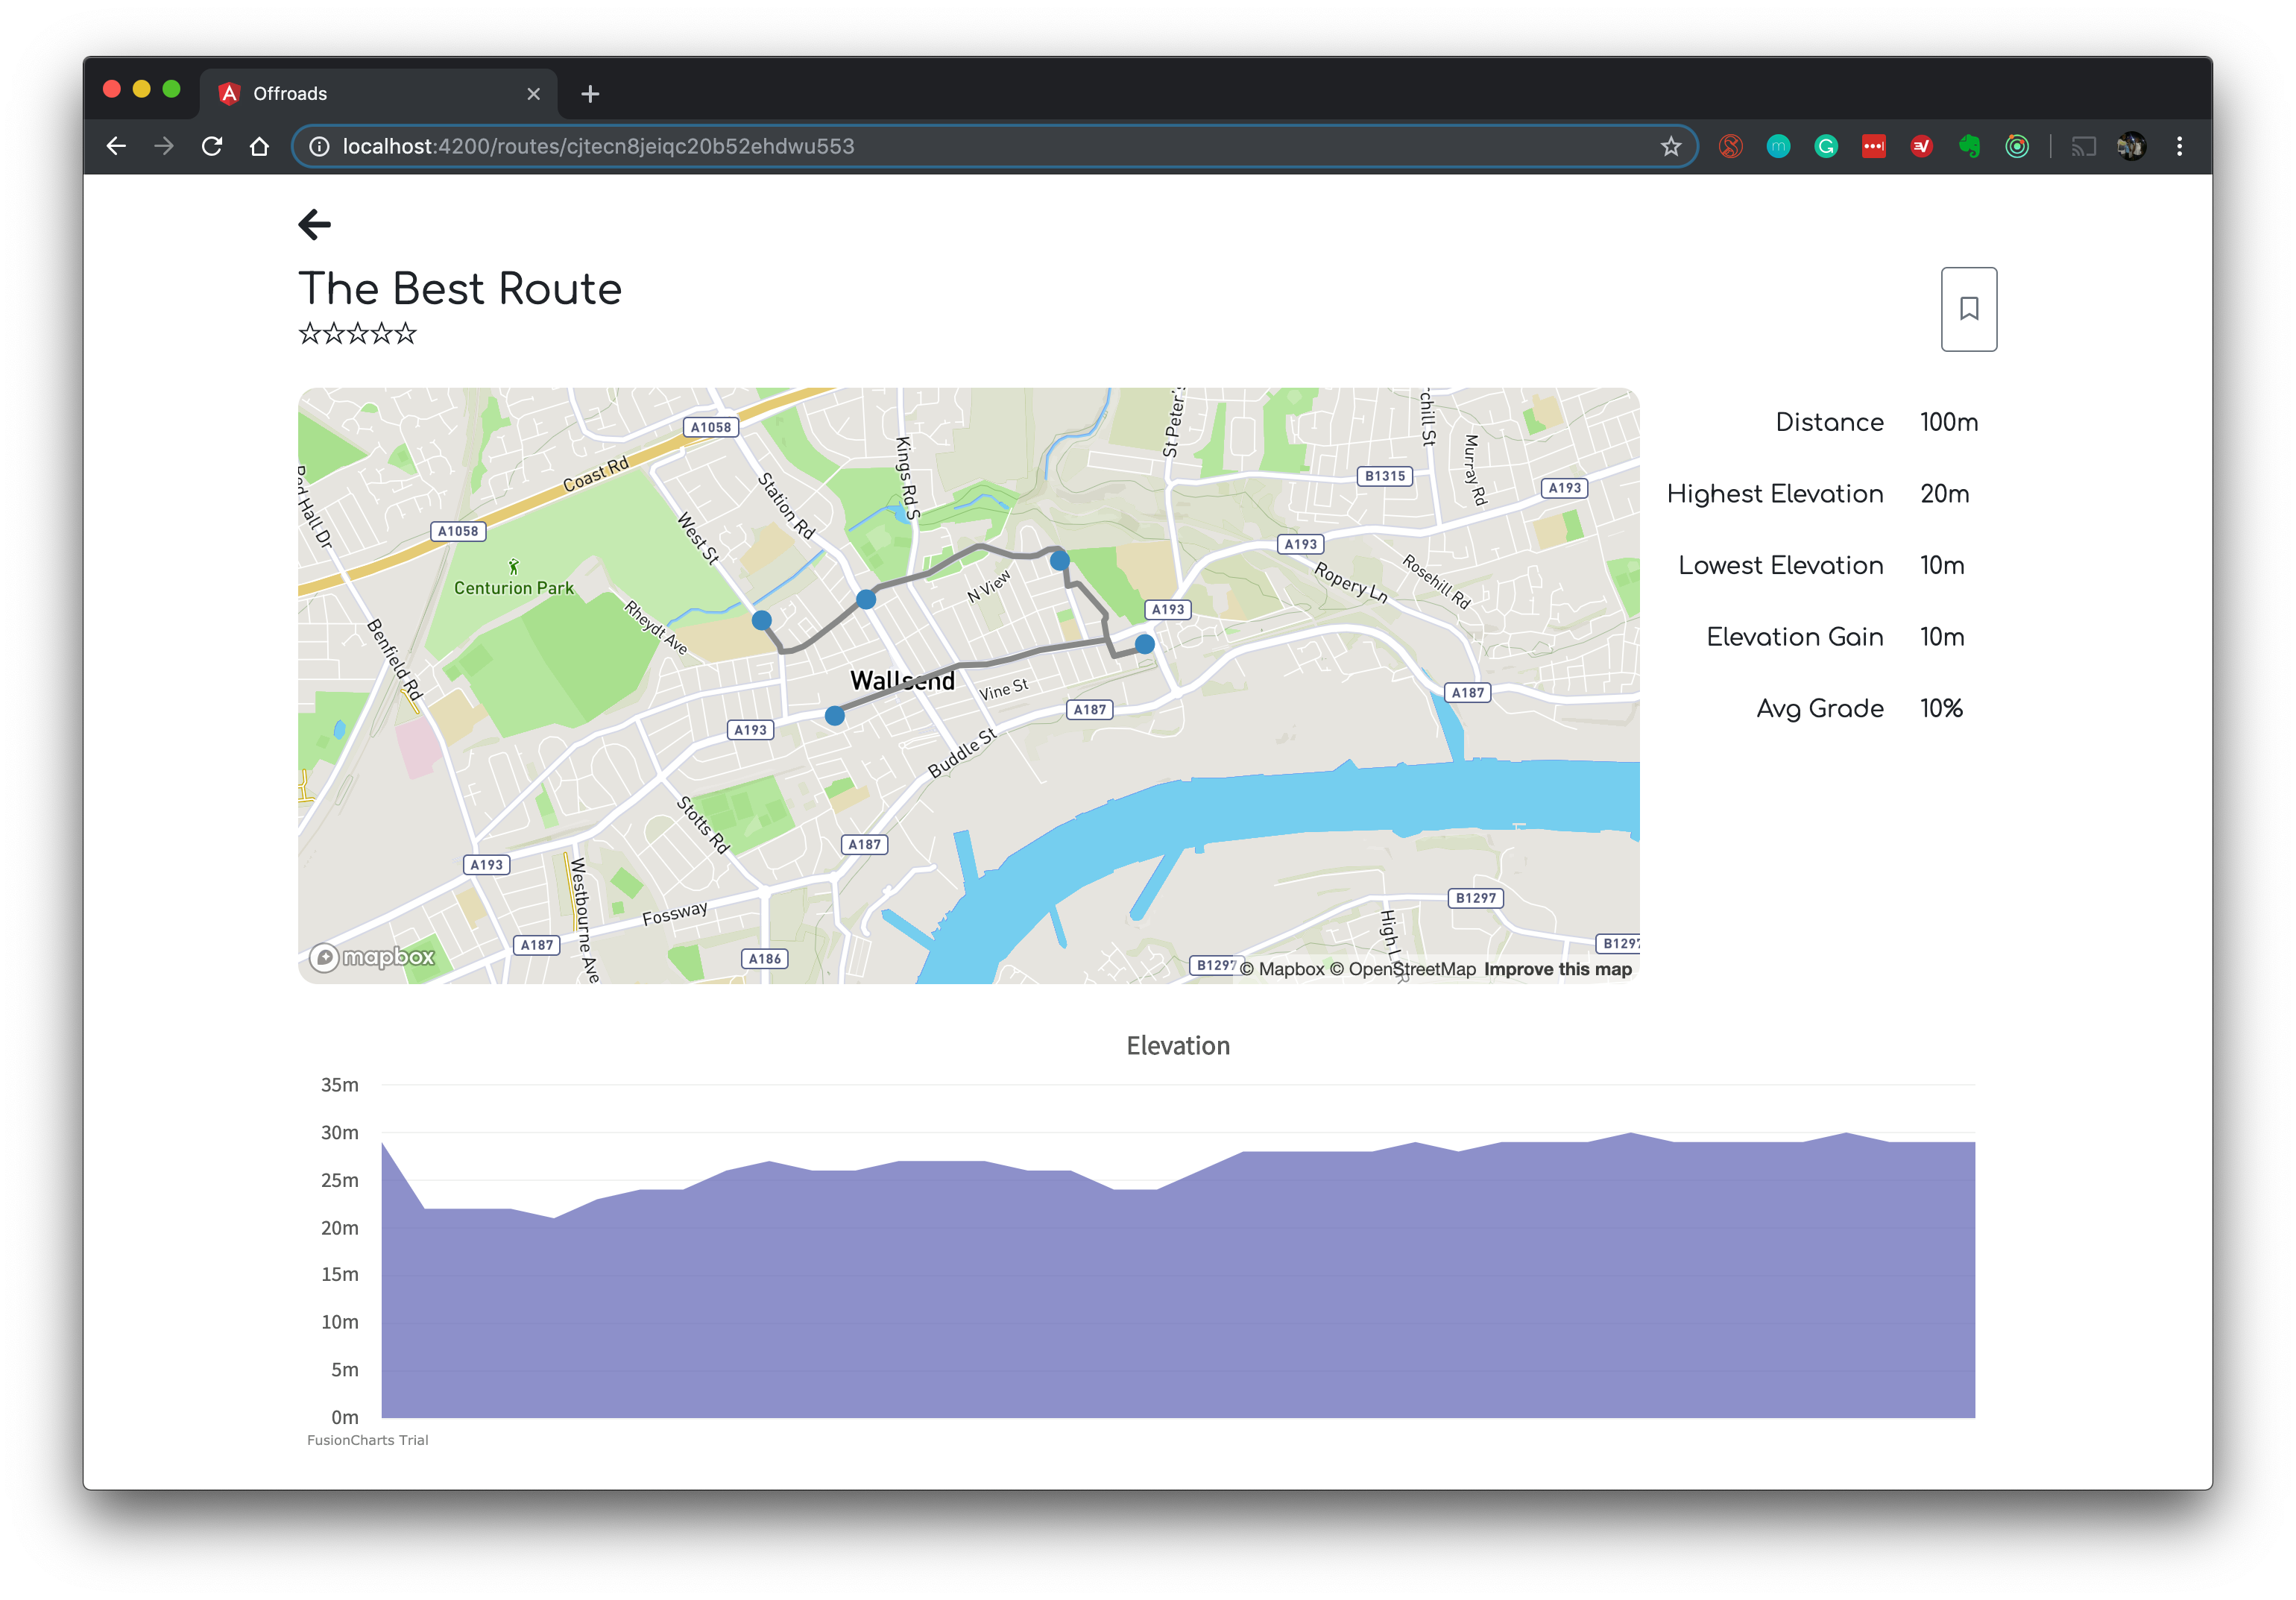
\includegraphics[width=0.75\textwidth]{trail-description.png}
    \caption{Trail description page. Note: details on the right side of map are placeholders and are not a reflection of the trail}
    \label{fig:trailDescriptionPage}
\end{figure}

\subsubsection{Enabling Competition}
An important feature that the system provides is a way of enhancing competition. It does so by allowing users to upload runs they have performed on a trail and the times for that specific run. These times are then used to rank the users in a leader-board as shown in \autoref{fig:leaderboard}. So users can compare their times against others when they run a trail and see where they place. 

\begin{figure}[htb!]
    \centering
    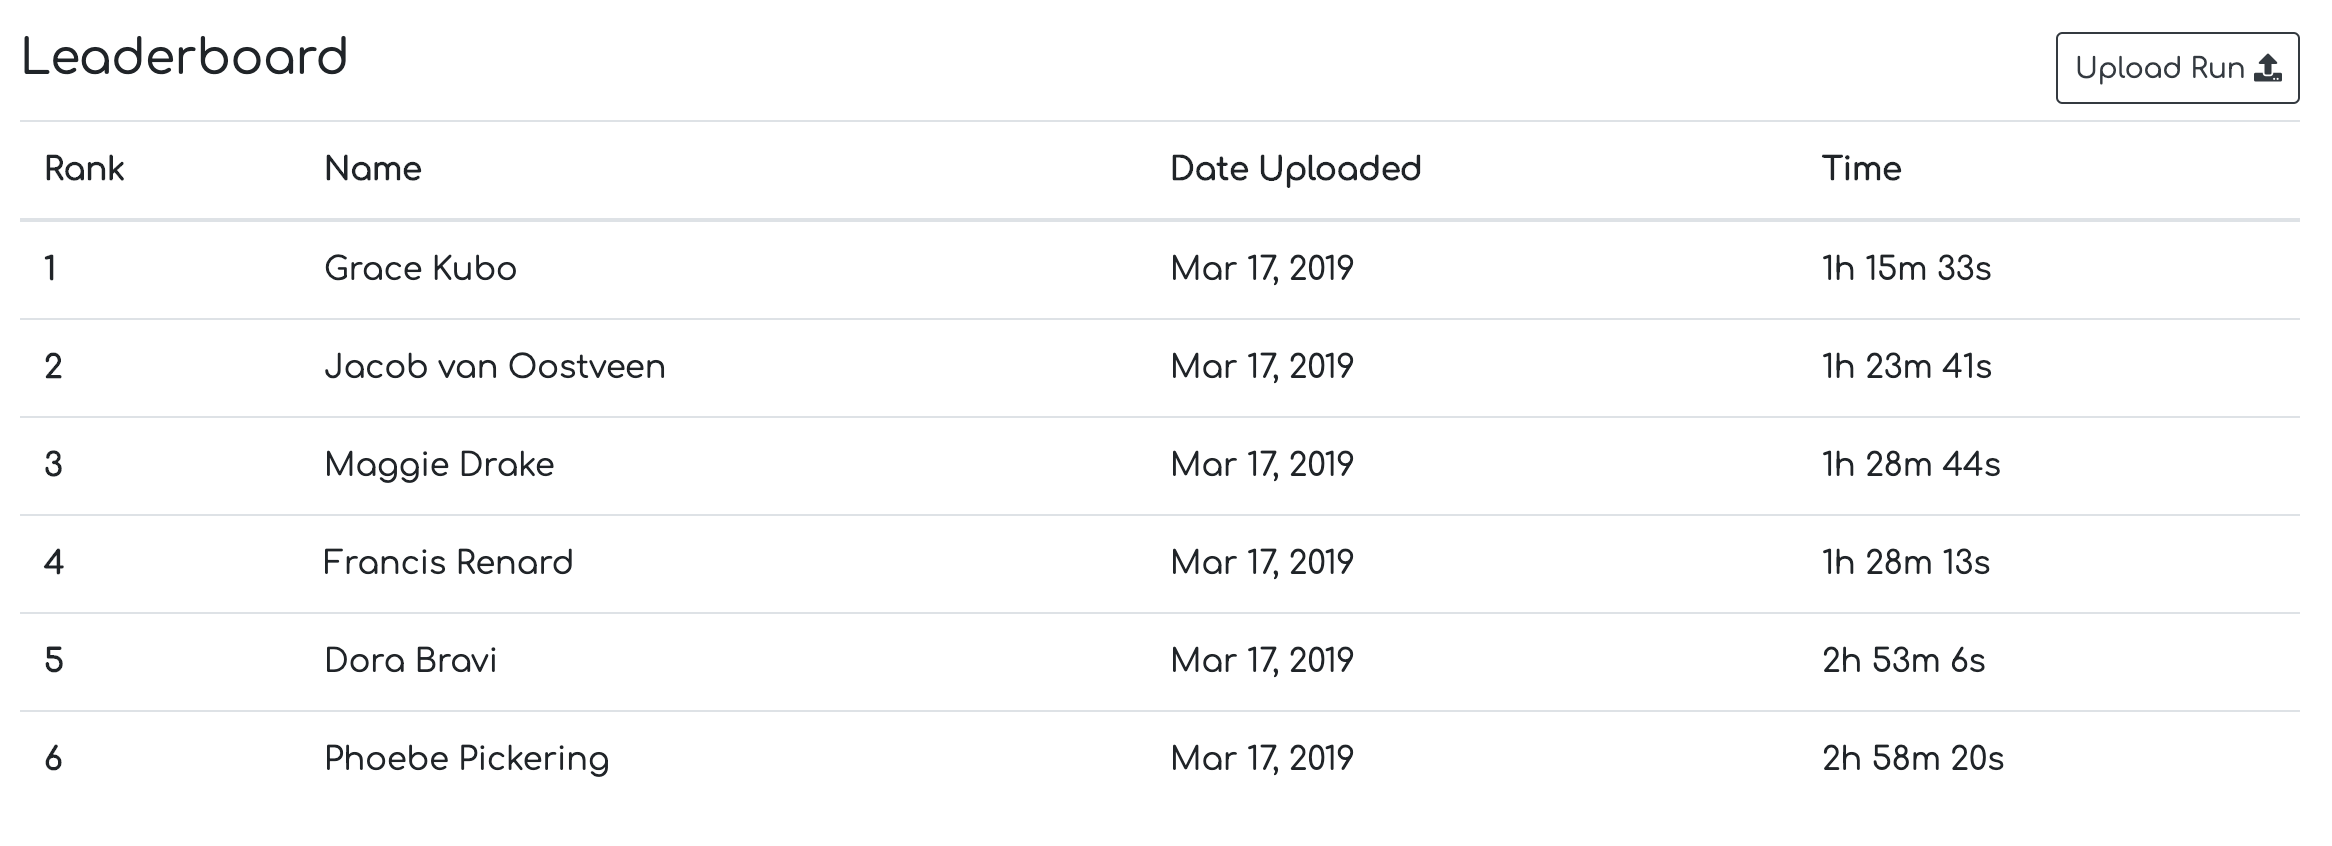
\includegraphics[width=0.75\textwidth]{leaderboard.png}
    \caption{Leader-board table on the trail description page}
    \label{fig:leaderboard}
\end{figure}

\subsubsection{Reviews and Ratings}
Users can review a trail that they have run and also give ratings for the trail. This is displayed on the description page to help advice users who want to run the current trail. The ratings are used to calculate the average rating of the trail and also used in the Recommender system discussed in \autoref{chap:Recommender}. The rating scale \cite{wright1982rating} from 1-5, 1 indicating strong dislike and 5 indicating strong like (see \autoref{fig:reviews}).

\begin{figure}[htb!]
    \centering
    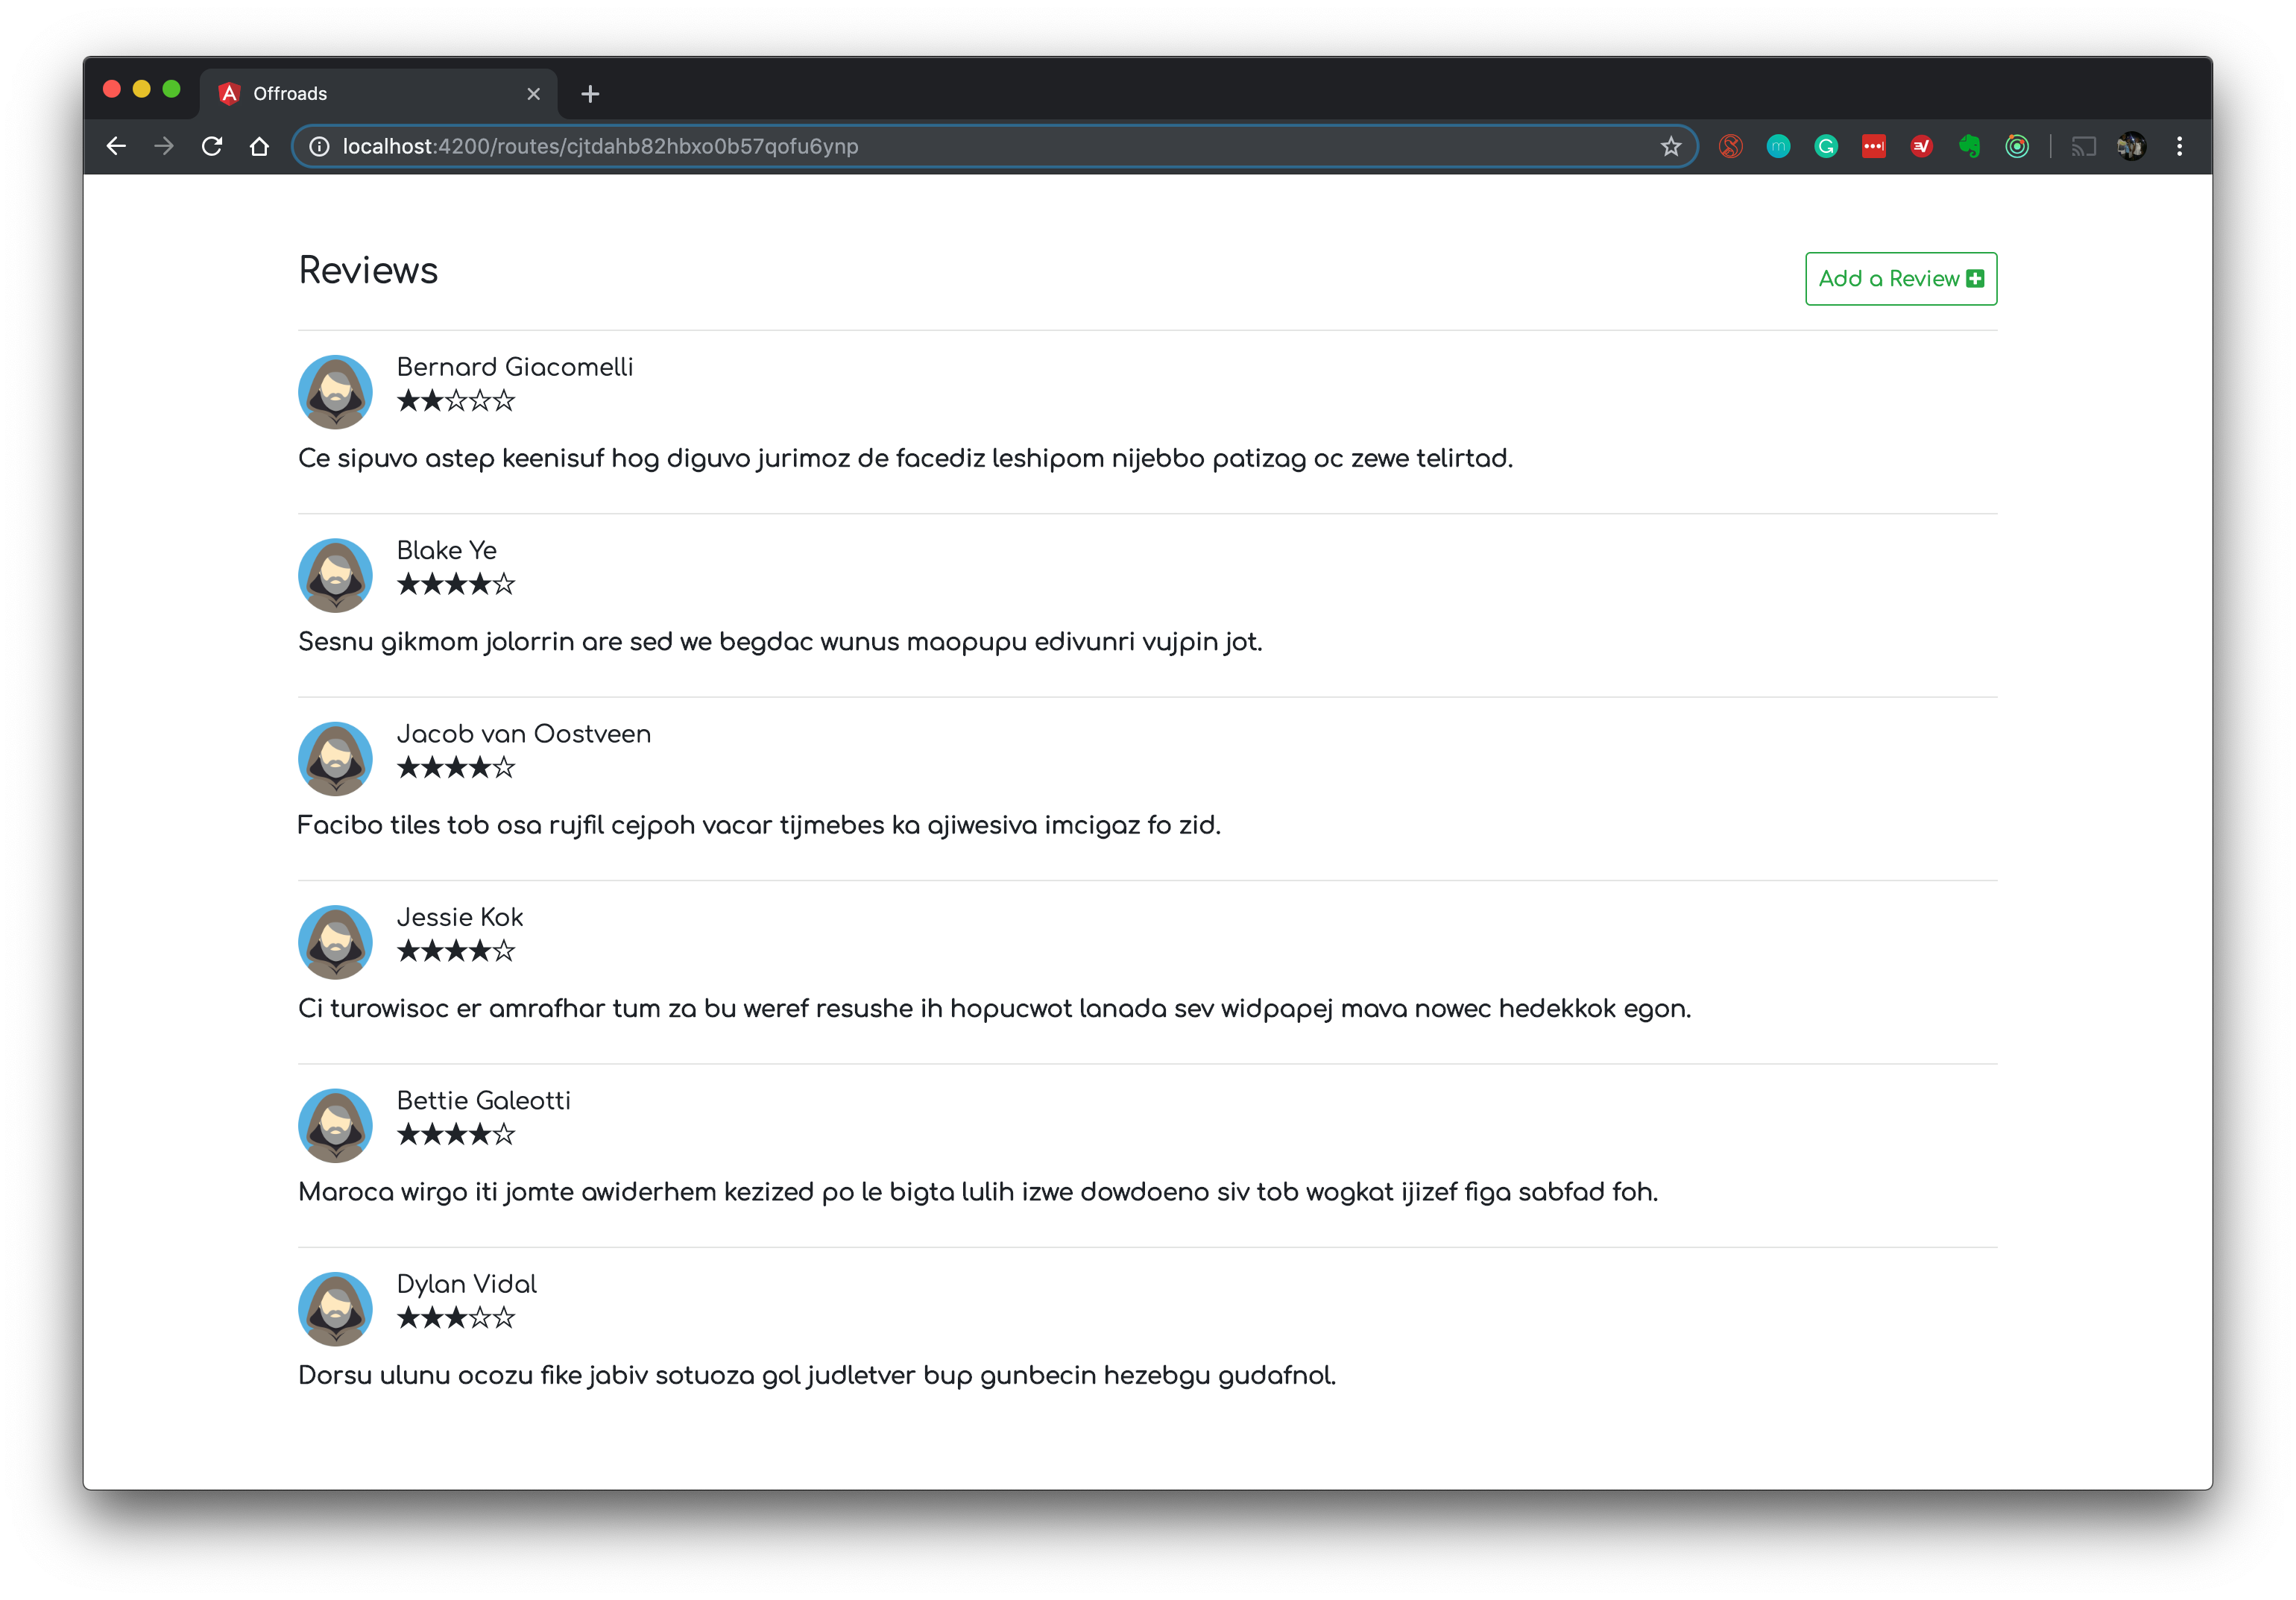
\includegraphics[width=0.75\textwidth]{reviews-ratings.png}
    \caption{(Randomly generated) user reviews and rations}
    \label{fig:reviews}
\end{figure}

\subsection{Feed page}
To enhance discovery, the system provides social media features in the form of a feed page. Users can follow other users of the web application. By doing this, the users feed page is populated populated with activities from the users they follow. They would be able to see the runs and routes created by the users they follow. This allows users to see new routes that they haven't ran before or see the runs other users have performed on routes, enabling for more discovery.

\begin{figure}[htb!]
    \centering
    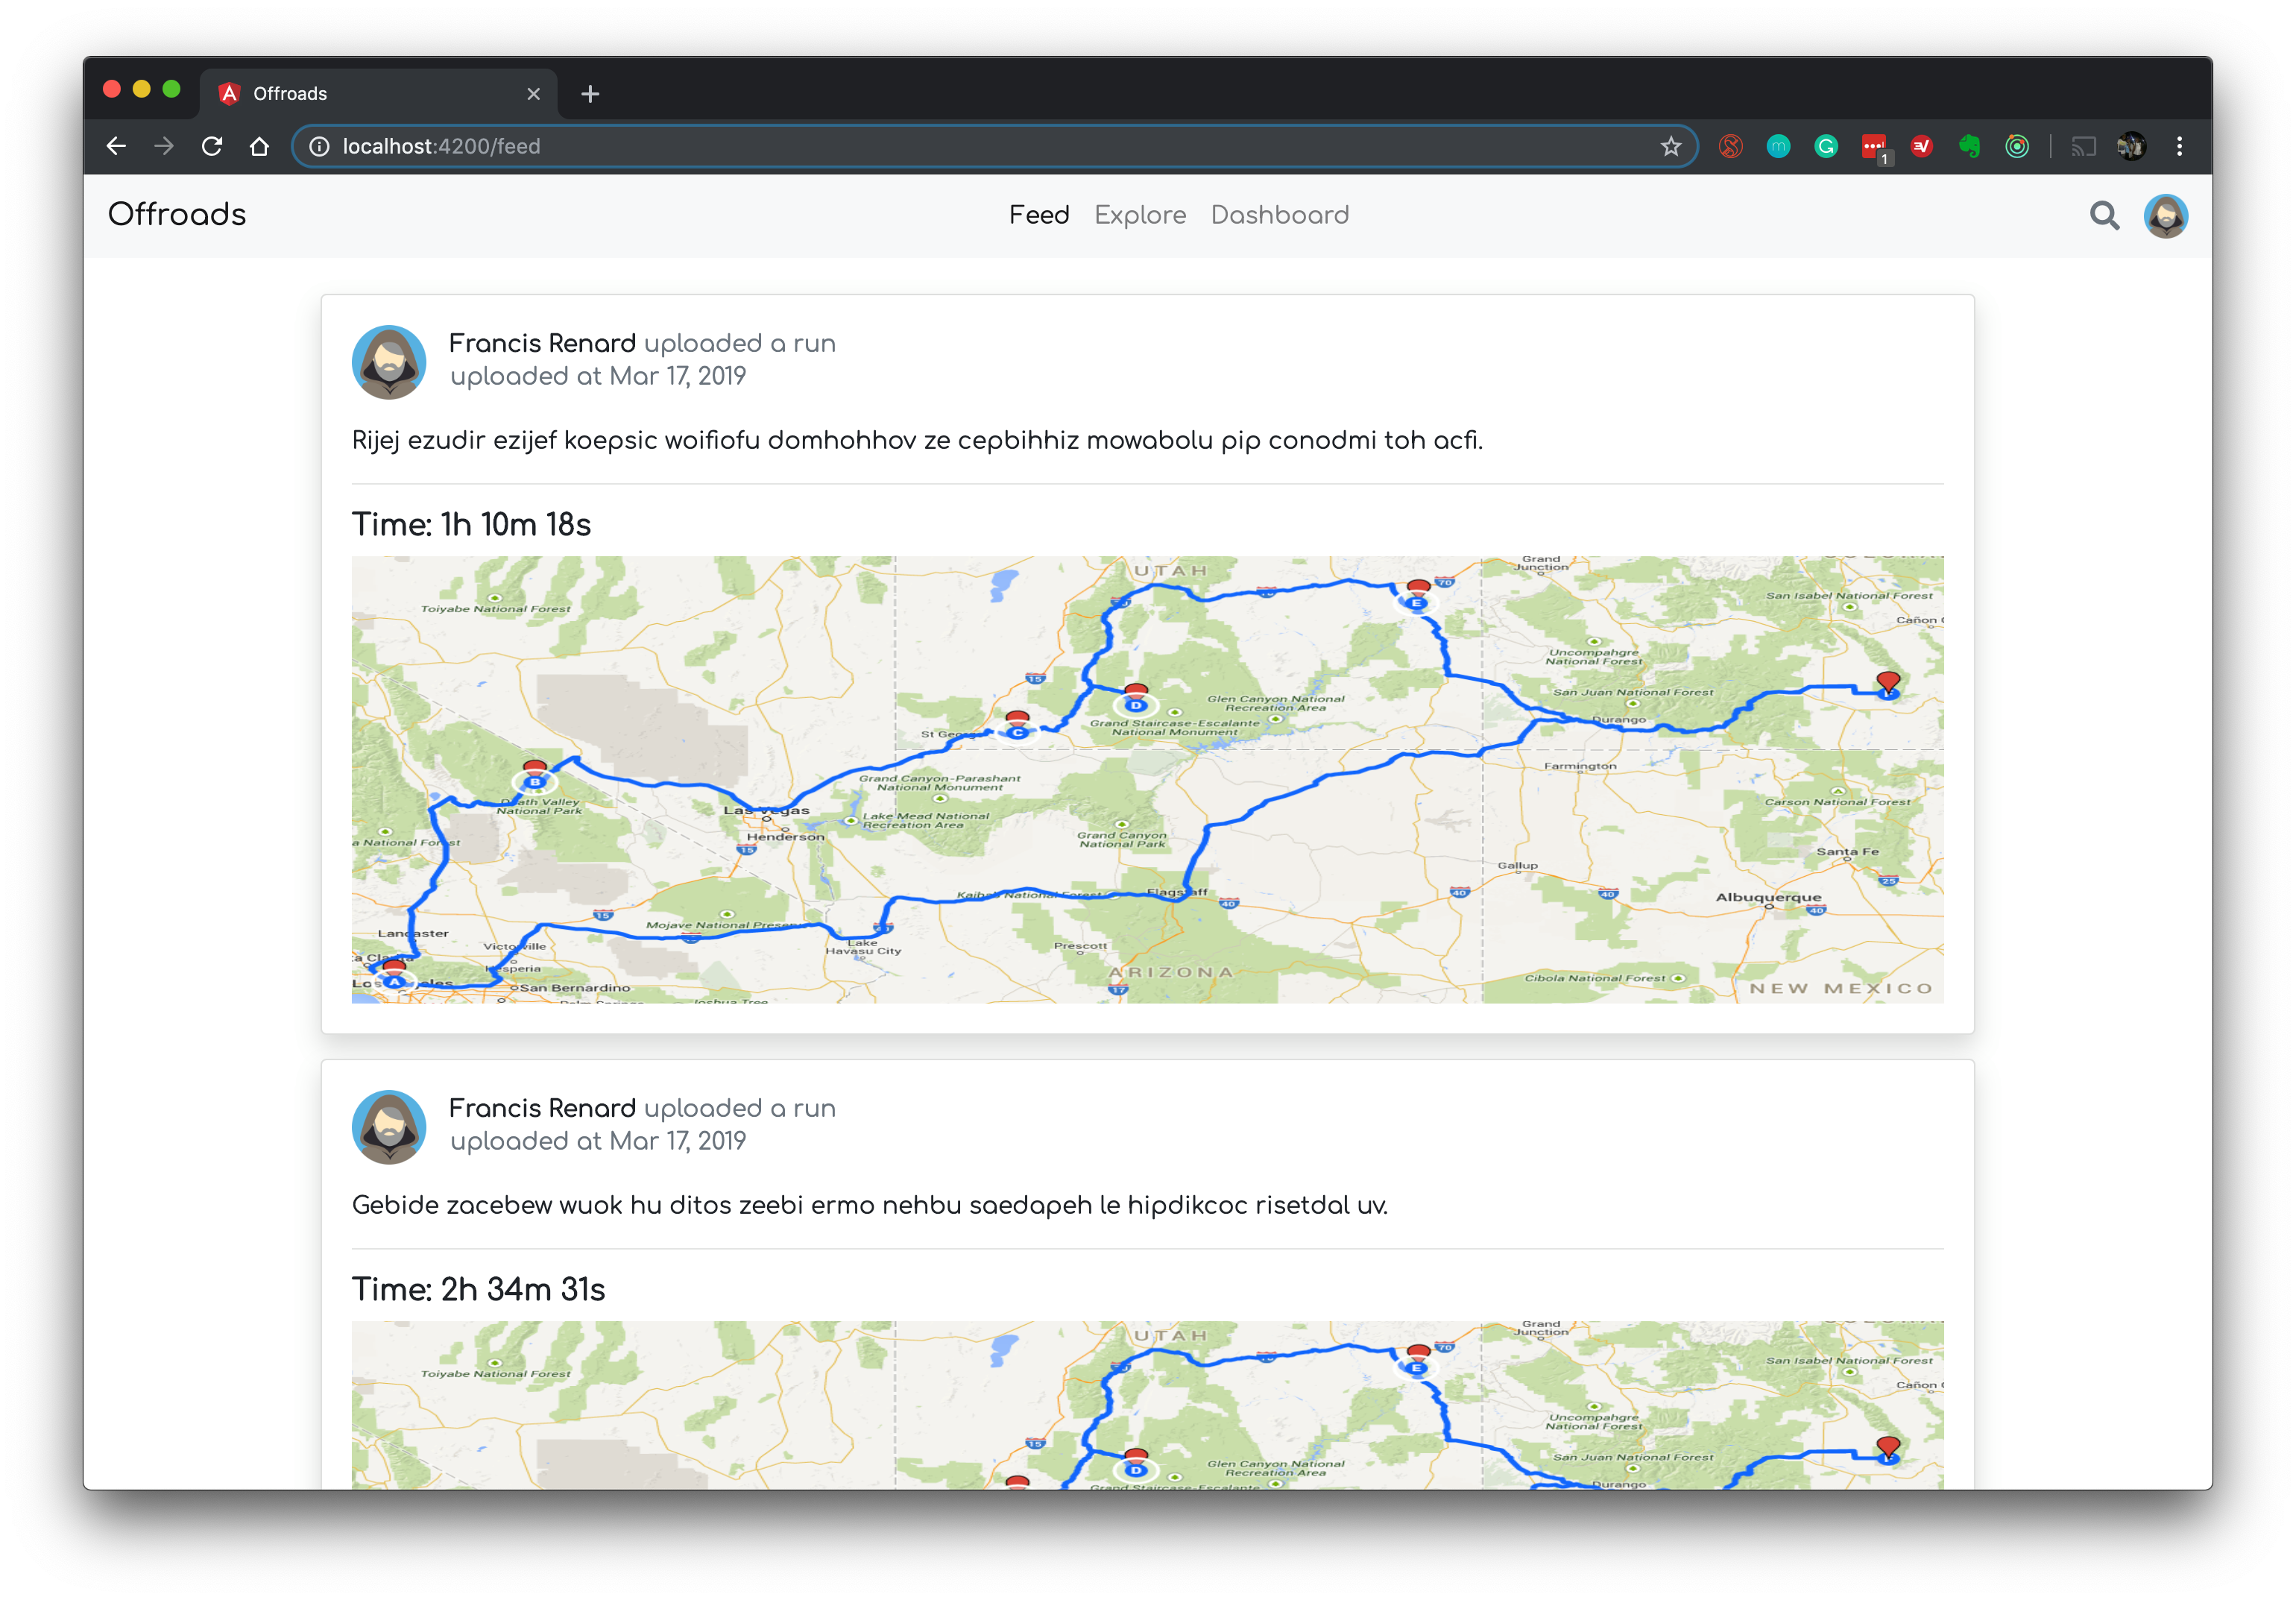
\includegraphics[width=0.75\textwidth]{feed-page.png}
    \caption{(Randomly generated) user feed page}
    \label{fig:feedPage}
\end{figure}





\chapter{Recommender System} \label{chap:Recommender}

This chapter will discuss the machine learning approach to building a Recommender system proposed in \autoref{sec:RecSystems}. It discusses the different approaches to creating this Recommender system and explains the reasons behind the chosen method.

\section{Information Gathering}
The Recommender System requires a representation of a users preferences in a format suitable for statistical analysis. To generate this representation, we need to collect some form of feedback from the users. There are three types of feedback that can be retrieved from the user.

\subsubsection{Implicit Feedback}
The user preferences are obtained automatically from implicit user actions on the system. This reduces the amount of work and input needed by the user, however it is less accurate. Implicit data we can collect is the number of times a user clicks on a trail, but a user clicking on a trail does not reflect their feelings towards that trail.

\subsubsection{Explicit Feedback}
The system requires users to reflect on the choices of trails that they make. In our system we provide a review system discussed in \autoref{subsec:trailDescription}, that asks users to rate the trails that they've run \cite{jawaheer2010comparison}. As the users provides this data explicitly, it is more accurate and more greatly reflects the users preferences. However, users are less likely to leave reviews and ratings unless forced too.

\subsubsection{Hybrid Feedback}
A combination of both Implicit and Explicit feed-backs, using the strengths of both and minimising the weakness of each feedback method. 

Due to the inaccuracy of implicit feedback, especially in our scenario, I decided to just rely on explicit feedback.

\section{Choosing A Recommender Algorithms} \label{chooseRecAlg}
There are multiple different ways of implementing Recommender system. For a machine learning approach, there are three popular approaches used which are
\begin{itemize}
    \item Content-based filtering
    \item Collaborative filtering
    \item Hybrid Technique
\end{itemize}
as shown in figure \ref{fig:recommenderSystemTypes}. The main feature that the approaches listed above is similarity.

\begin{figure}[htb!]
    \centering
    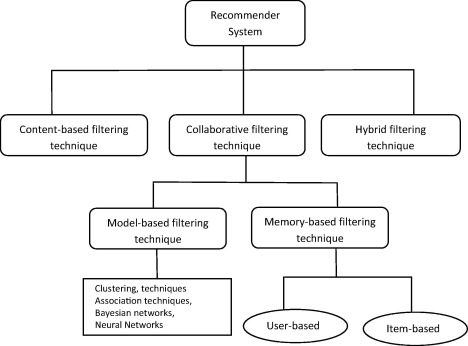
\includegraphics[width=0.5\textwidth]{recommenderSystemTypes.jpg}
    \caption{Types of Recommender Systems \cite{isinkaye2015recommendation}}
    \label{fig:recommenderSystemTypes}
\end{figure}

\subsubsection{Content-based filtering}
\acrfull{cbf} recommends items based on information known about the particular item \cite{pazzani2007content}. The system would have some meta-data about the item, for example, in our scenario we would have extra information about trails such as the type of terrain, location, elevation etc. Items are recommended to the user based on features extracted from users history of positively rated items that represents a users preferences \cite{isinkaye2015recommendation}.

\acrshort{cbf} resolves some of the problems of \acrshort{cf}. The system can still recommend items to users who have not rated any items \cite{burke2002hybrid}. However the the strength of the system greatly relies on how well the content analysis is. 

Content Analysis is the technique of mapping symbolic data into data in a matrix format suitable for analysis \cite{roberts2001content}. For some domains such as news and publications it is quite effective, but for user data that is quite subjective and can be influenced by a large number of variables, it can be difficult and the attributes retrieved may not be suitable to categorise a trail. Having the user add attributes to trails is not a very user friendly method as users are not inclined to perform such menial tasks.
 \ref{fig:contentBasedFiltering}
\begin{figure}[htb!]
    \centering
    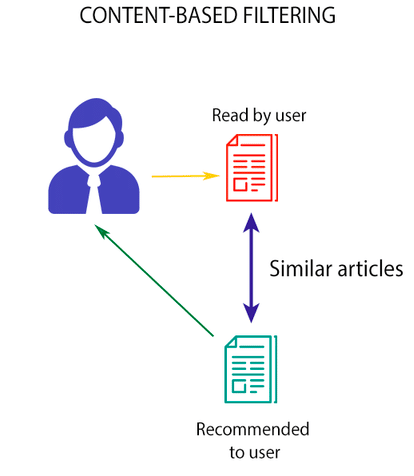
\includegraphics[width=0.5\textwidth]{content-based-filtering.png}
    \caption{Content-based filtering \cite{contentFiltering}}
    \label{fig:contentBasedFiltering}
\end{figure}

\subsubsection{Collaborative filtering}
\acrfull{cf} is a domain independent technique especially useful when content analysis of the items cannot be easily done \cite{isinkaye2015recommendation}. It does so by matching users that are similar based on the user preferences and using this matching to make recommendations \cite{herlocker2004evaluating}. The idea is that, user A likes routes 1 \& 2 and user B likes routes 2 \& 3. As user A and user B like the same route (route 2), then they are similar and user A would also like route 3. 

This property can be seen in real life and works extremely well. People are more likely to trust the suggestions of their friends, i.e. people that they are the most similar with. With this system, you do not need to know any extra information on the routes you are running the algorithm on. We us either explicit information such as user ratings, or implicit information such as number of views on a route, to determine the routes users like. Example shown in figure \ref{fig:collaborativeFiltering}.

\begin{figure}[htb!]
    \centering
    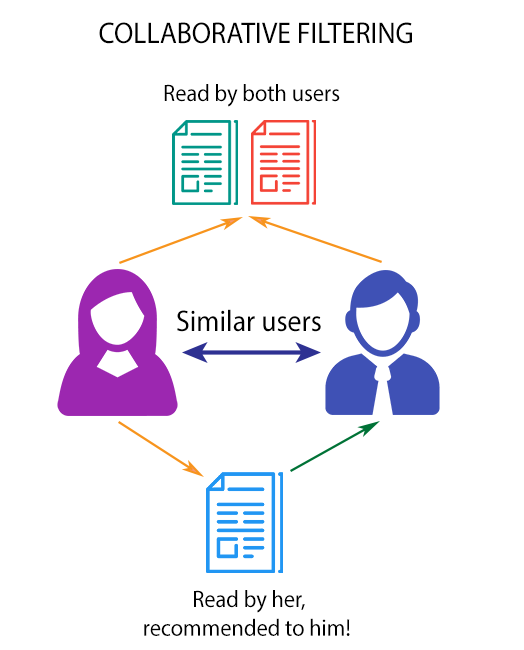
\includegraphics[width=0.5\textwidth]{collaborative-filtering.png}
    \caption{Collaborative filtering \cite{collabFiltering}}
    \label{fig:collaborativeFiltering}
\end{figure}

As trails are quite hard item to perform content analysis on, I decided to chose the collaborative filtering technique. It is best suited to trail running as users are more likely to run routes recommended to them by others.

\subsubsection{Hybrid Recommender Systems}
Hybrid Recommender systems simply combine the results of both collaborative and content-based techniques \cite{claypool1999combing}. The results from both the system's would then have to be ranked again in the combiner as shown in figure \ref{fig:hybridRecommenderSystems}

\begin{figure}[htb!]
    \centering
    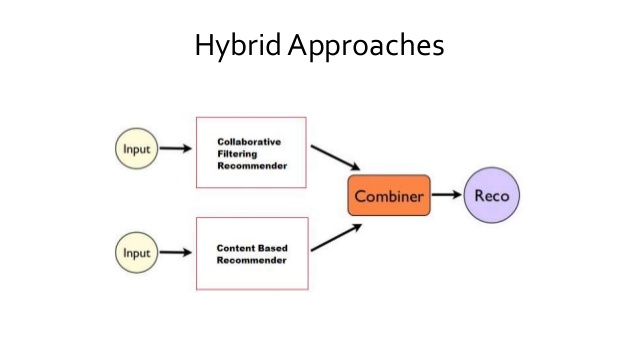
\includegraphics[width=0.5\textwidth]{hybrid-approaches.jpg}
    \caption{Hybrid Approaches \cite{hybridrecommender}}
    \label{fig:hybridRecommenderSystems}
\end{figure}

Although this may be a more appropriate approach to building Recommender Systems, it still requires the complexities from content-based filtering, hence this approach was not used. For this reason, we use a \acrlong{cf} Technique.

\section{Collaborative Filtering}
Collaborative filtering techniques require the system to find users that are similar based on their user preferences inferred from the ratings they give trails they have run previously. There are 2 main approaches to collaborative filtering. We compare these methods below to decide which method is is best suited to our application.

\subsubsection{Memory based Technique}
Memory based based techniques calculate a similarity scores between users or between trails based on the ratings users give trails  \cite{wang2006unifying}. It uses statistical calculations such as the Pearson Correlation Coefficient \cite{benesty2009pearson}, or the Cosine Similarity \cite{michie1994machine}, to calculate the similarity which is weighted against the ratings provided to recommend and rank trails to new users.

This method struggles with performance as the calculations have to be calculated for each individual user on every request. This creates a bottleneck, slowing down the system to perform these calculations. It also means that the system is not very scalable, as users grow, the system will slow down even more. Another issues is the system cannot adjust to user changes quickly. The lack of a model being trained means the system cannot adjust to changes in user preferences.

\begin{figure}[htb!]
    \centering
    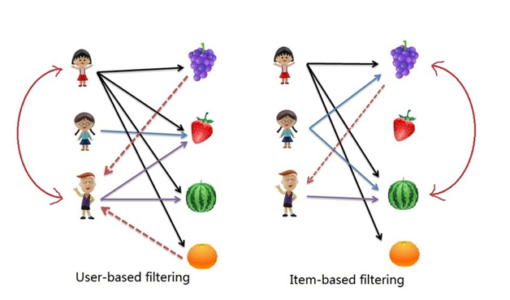
\includegraphics[width=\textwidth]{collab-filtering-types.png}
    \caption{Memory based techniques to collaborative filtering \cite{collabFilteringTypes}}
    \label{fig:collabFilteringTypes}
\end{figure}

\subsubsection{Model based techniques}
To improve on the issues of the memory based techniques, we can use model based techniques. We create a machine learning model that will be trained on a data set of user-trails ratings using the Matrix Factorisation method described in section \ref{matrixFactorization}. We will use a neural network described in section \ref{neuralNetwork}

\section{Matrix Factorisation} \label{matrixFactorization}
To be able to predict trails that would be most suitable to a user, the system needs to learn two main features about the users and trails:
\begin{itemize}
    \item what features a specific user likes in trails
    \item what features a route has that users like
\end{itemize}
We can learn these features using a method called Matrix Factorisation, which is one of the top methods proposed during the Netflix Prize \cite{bell2007lessons}.

We can convert our user-trails ratings from our database into a user-trail matrix. Matrix Factorisation is the process of decomposing a user-trail rating matrix into a product of 2 lower dimension rectangular matrices \cite{koren2009bellkor} as shown in figure \ref{fig:matrixFactorization}.

\begin{figure}[ht]
    \centering
    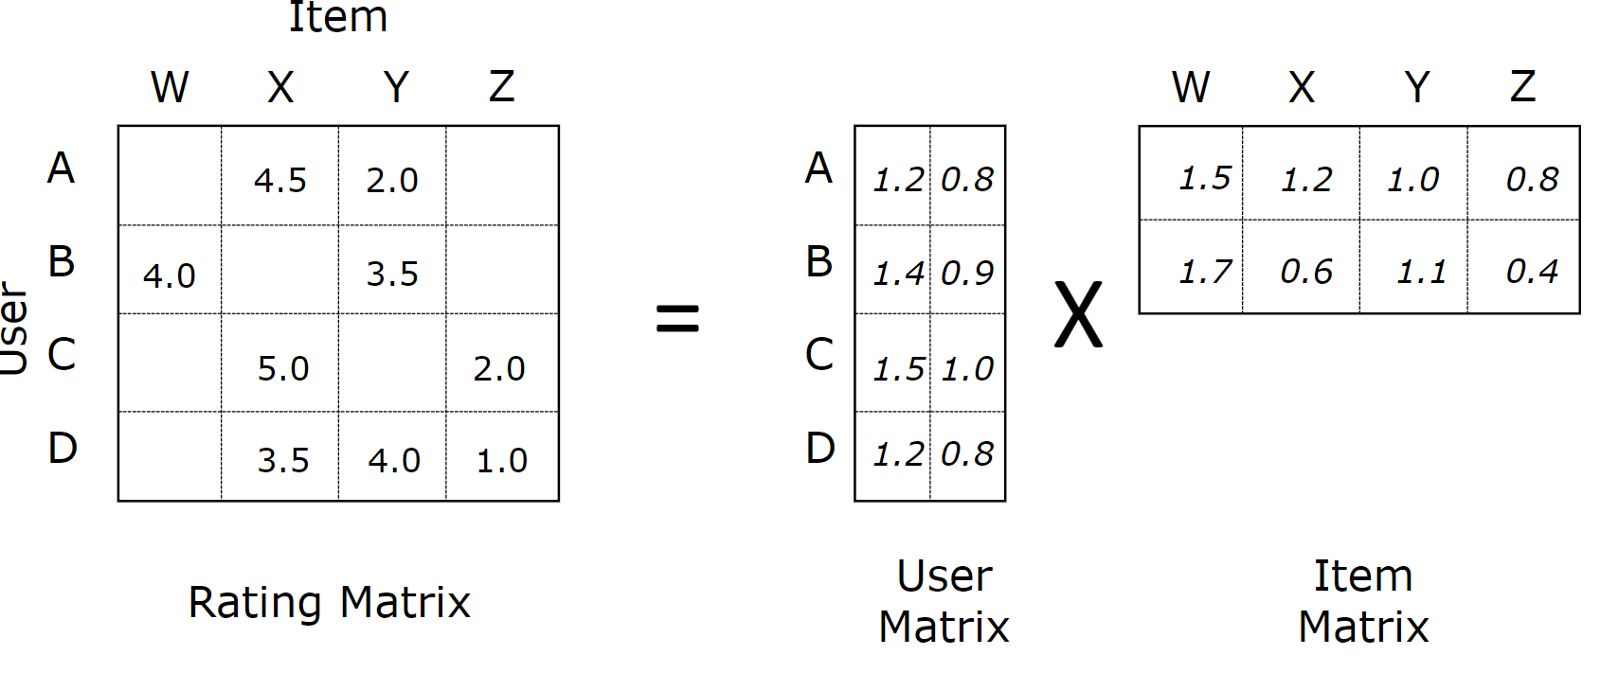
\includegraphics[width=\textwidth]{matrix-factorization.png}
    \caption{Example of Matrix Factorisation}
    \label{fig:matrixFactorization}
\end{figure}

We can represent the above mathematically as 
\begin{equation}
    R \approx P \times Q^T
\end{equation}

Where $R$ is our ratings matrix of size $i \times j$, where $i$ is the number of users and $j$ is the number of trails. $P$ is a user-feature matrix of size $i \times k$ where $k$ is the number of features. $Q$ is a trail-feature matrix of size $u \times k$ and $Q^T$ is its transposition.

As the lower dimension matrices are a decomposition of the ratings matrix, they represent the factors that users use to decide their ratings. Our goal is to find the values for these lower dimension matrices that best describe the ratings matrix and hence best describe the users and trails. These matrices in essence become our user preferences and trail attributes.

These features are also known as \Gls{latent} features because, we do not know explicitly what the features are or even if they exist. The values in the feature matrices could represent the terrain of a trail, or the pollution around the trail, or any feature, however, without rigorous analysis of these values, we can not draw any conclusions as to what they mean.

This does mean that we do not really know the reasons why users like certain trails and we cannot share that back to the user or use that in any other analytic methods. However, this does not in anyway affect the accuracy of the Recommender system. 

To optimise the values in our lower dimension algorithms, we need to calculate how wrong our initial predictions are from our initial matrices. We calculate this loss value using a Loss function. This is then used to update our matrices towards their optimal value using Gradient Descent.



\subsection{Learning Process}
Our initial lower dimensional matrices are initialised to random values. The learning process is to optimise the values of the lower dimension matrices such that the predicted values calculated for ratings are close to the original matrix ratings values. Hence for each $r_{ij} \in R$ we want to calculate $\hat{r_{ij}}$:

\begin{equation}
    \hat{r_{ij}} = p_i \times q_j^T = \sum_{k=1}^{k}{p_{ik}q_{jk}}
\end{equation}

To optimise this we first need to calculate our loss value. This indicates how far away from the actual value our predicted value is

\subsubsection{Loss Function}
A loss function\footnote{also known as a cost function} is a statistical mapping of the correctness of an event or value \cite{wald1950statistical}. Loss functions are a big part of machine learning models as they allow us to empirically evaluate a the model as discussed in \autoref{subsec:evaluationMetrics}. They are also used to train the models, used in the learning phase to discover how our values need to be optimised. 

Choosing a loss function depends on the type of problem you wish to solve and also require a lot of experimentation. From \autoref{subsec:mlApproach}, we know that our Recommender systems can be categorised as a Regression Analysis for regression problems. The loss function we use is called the \acrfull{mse}.

The mean squared error is the measure of an average of the square differences between the predicted values of and the actual values.

\begin{equation} \label{eqn:mseLossFunction}
    MSE = \frac{1}{N}\sum_{i=1}^{N}{({p_i}-{a_i})}^2 
\end{equation}

Where $N$ is the number of iterations performed when training our model. $p_i$ is our predicted value for the $ith$ iteration and $a_i$ is the actual value. Squaring this value has two benefits. It makes the value absolute, as we only care about the difference and not the sign. It also ensures that our loss van be modelled as a quadratic functions. This benefits the system as it ensures there is only one minimum value, (one optimised value). This gives the allows us to easily know when the system has reached the best optimisation possible without over-shooting the minimum.

\subsubsection{Gradient Descent}
Gradient descent is an optimisation algorithm that aims to minimise a loss function by repeatedly taking descent learning steps over a negative gradient towards a minimum value. The gradient descent algorithm takes in a learning rate. This tells us the size of the learning steps we take. 

\begin{figure}[ht]
    \centering
    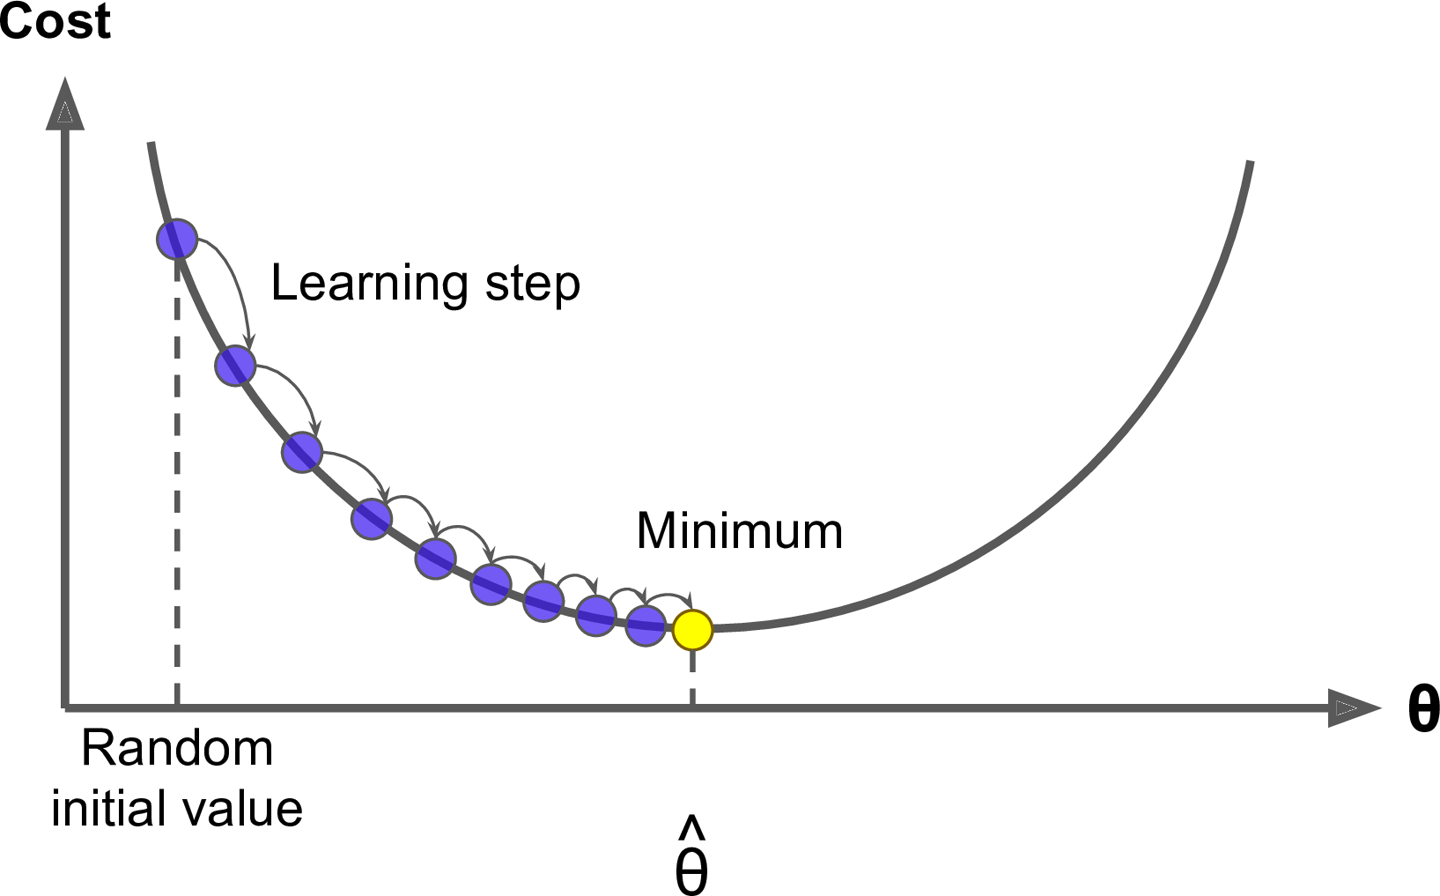
\includegraphics[width=0.75\textwidth]{gradient-descent.png}
    \caption{Gradient Descent \cite{gradientDescent}}
    \label{fig:gradientDescent}
\end{figure}

The gradient descent algorithm used is called \acrfull{adam} which is a variant of \acrfull{sgd}. In gradient descent, we train our model in batches, the number of samples used to train the model during a single iteration. \acrshort{sgd} is a way of performing large-scale machine learning with large data sets and sample sizes \cite{bottou2010large}. It does so by randomly shuffling the sample size and using one sample size per iteration, using the result of that to estimate the others. This generally means that it's more noisy and we need smaller learning steps, but it does not affect the learning process and reduces computation need.

\acrshort{adam} is based on adaptive estimates and lower-order momentum first published in 2014 \cite{kingma2014adam}. It is a complex technique that even further increases the speed of training.

\subsection{Improving with Bias}
To improve our model, we can introduce bias. In real life, you would trust a user that has run more trails than a user that has run fewer routes. This also applies for routes that have been run by more users. We can include this feature into our model to help improve the model created by adding bias values related to each user and each item (route). We include this bias in when training our model. Our new predicted ratings $\hat{r_{ij}}$ can be calculated as

\begin{equation}
    \hat{r_{ij}} = b_i + b_j + {q^{T}_{j}}{p_i}
\end{equation}

Where $b_i$ is our user bias and $b_j$ is our trail bias.

\section{A Deep Learning Approach} \label{neuralNetwork}
Deep learning is a category of machine learning that based on Artificial Neural Networks. Neural networks is a framework for modelling solutions to common machine learning problems based on the brains biological networks \cite{van2018artificial}. 

Neural networks consist of:
\begin{itemize}
    \item An input layer which has our initial input values.
    \item One or more hidden layer that take in as inputs, the values of the nodes from the previous layer and a weight the represents the strength between the current node and the previous node. Each node in this layer uses an activation function to output a value.
    \item An output layer, which will have our final predictions.
\end{itemize}

\begin{figure}[ht]
    \centering
    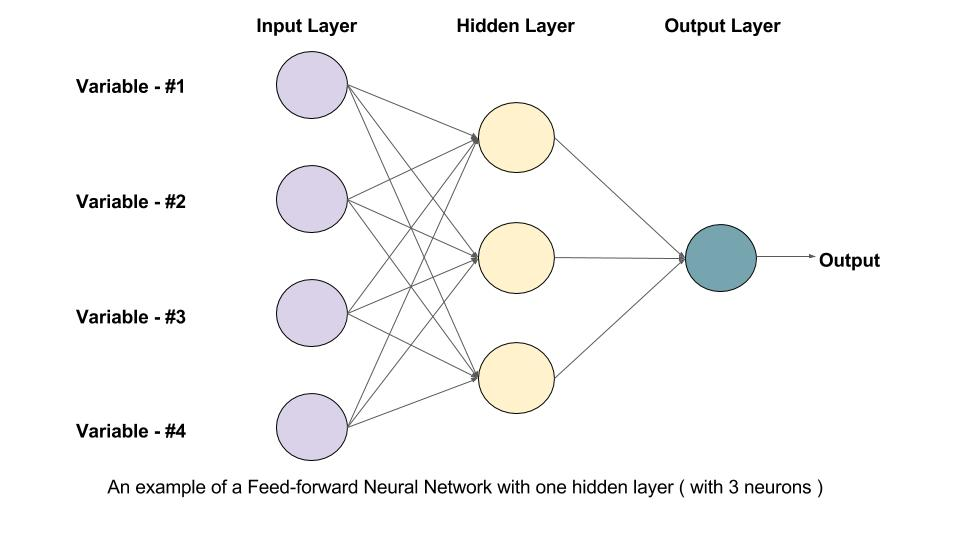
\includegraphics[width=0.7\textwidth]{neural-net-example.jpg}
    \caption{Neural Network Example \cite{neuralNet}}
    \label{fig:neuralNetworkExample}
\end{figure}


We can create our model discussed in section \ref{matrixFactorization}, using a neural network, making the model more robust. The user and and items feature matrices are flattened and concatenated to form our input layer. Then a fully connected hidden layer, that is each node in the hidden layer is connected to every node of the input layer. The hidden layer uses a ReLU activation function \cite{li2017convergence}. Lastly, an output layer with one node that we use to calculate our loss function. Each node also have a bias value that is added in the activation function calculation. The approach used hear was based of a lecture from Jeremy Howard \cite{jeremy2016deep}.

\subsection{Preventing over-fitting}
One of the main problems with machine learning approaches is over-fitting and under fitting.

\paragraph{Under-fitting} is a problem that occurs when the model does not fit the data it's trained on. This happens when not enough iterations has been performed during training making our loss function value worse.

\paragraph{Over-fitting} is when our model is trained to match to perfectly with our training data-set and therefore has a hard time to predict when we have a completely new data. To prevent this in Neural Networks we can add a dropout layer to the neural network. Drop out layers kill random nodes in our neural network during each epoch. This forces the neural network to always try and learn new paths to during training preventing it form relying on the same weights each time.

\begin{figure}[ht]
    \centering
    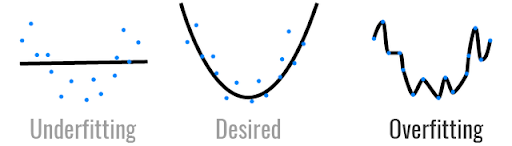
\includegraphics[width=\textwidth]{fitting-problem.png}
    \caption{Fitting Problems \cite{overfitting}}
    \label{fig:fittingProblems}
\end{figure}


\begin{figure}[ht]
    \centering
    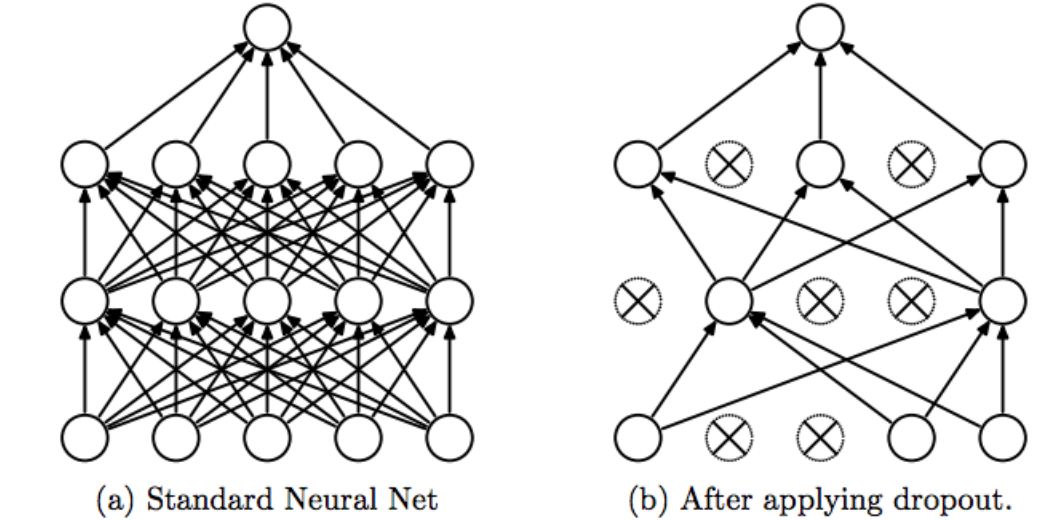
\includegraphics[width=\textwidth]{dropout.png}
    \caption{Dropout Layer \cite{dropout}}
    \label{fig:dropoutLayer}
\end{figure}
\section{Tensorflow and Python}
There are a few machine learning platforms that can help us to create our neural network. I decided to use Tensorflow because it is popular and has a big community to help. It also is built with keras which allows you to create these models from a High Level. Tensor flow also has C++ bindings that takes use of the GPU for the matrix which is far more efficient than using a normal CPU and so is quicker for handling large data-sets.

Tensorflow is mainly meant to be used in python as python is the main language for Data Science. This proved to be a problem initially as I did not know python. Although Tensorflow also provides a JavaScript library\footnote{https://www.tensorflow.org/js}, I chose to use the python version as the JavaScript library did not provide all the functionality of the main python library. It also allowed me to use Jupyter Notebook (discussed in section \ref{jupyterNotebook}) which provided a really platform to experiment with the machine learning model.

\begin{figure}[ht]
    \centering
    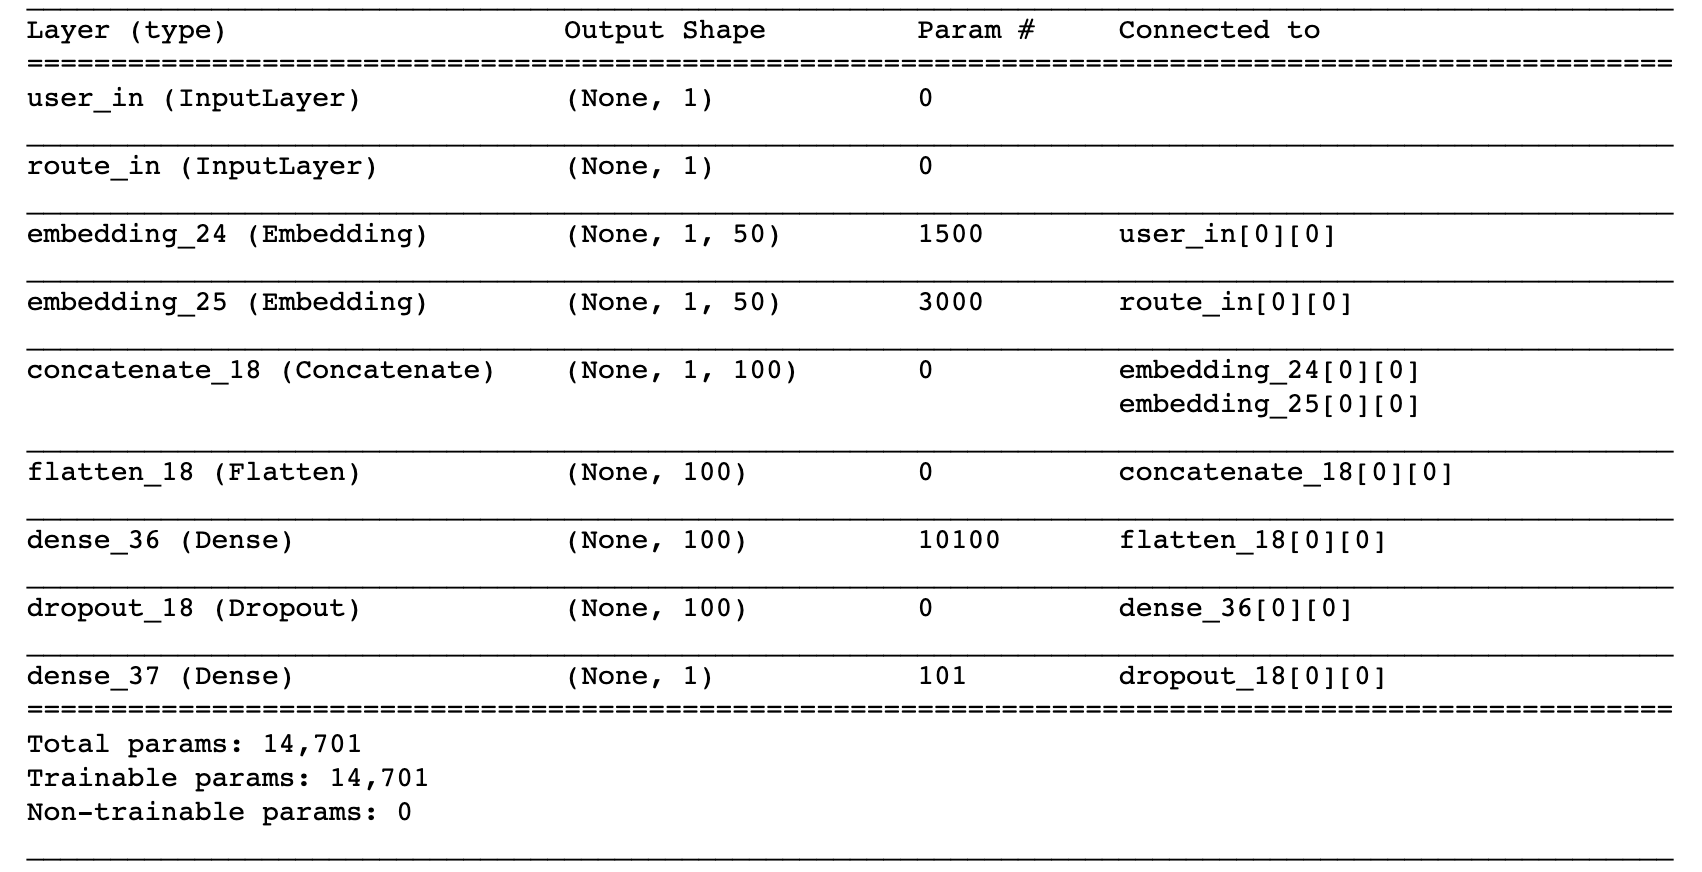
\includegraphics[width=\textwidth]{neural-net-summary.png}
    \caption{Summary of Neural Network}
    \label{fig:neuralNetworkSummary}
\end{figure}

\subsection{Jupyter Notebook} \label{jupyterNotebook}
Jupyter Notebook\footnote{https://jupyter.org/} that allows creating and running notebooks via a web application. These documents can contain both Markup text and more importantly code that is exists in cells on the document. The document allows you to easily share any code with others easily as it make's it straightforward to document. With it's use of cells, you can rerun individual blocks of code with running the entire document, making it easy to develop and iterate through different versions as you improve.
\begin{figure}[ht]
    \centering
    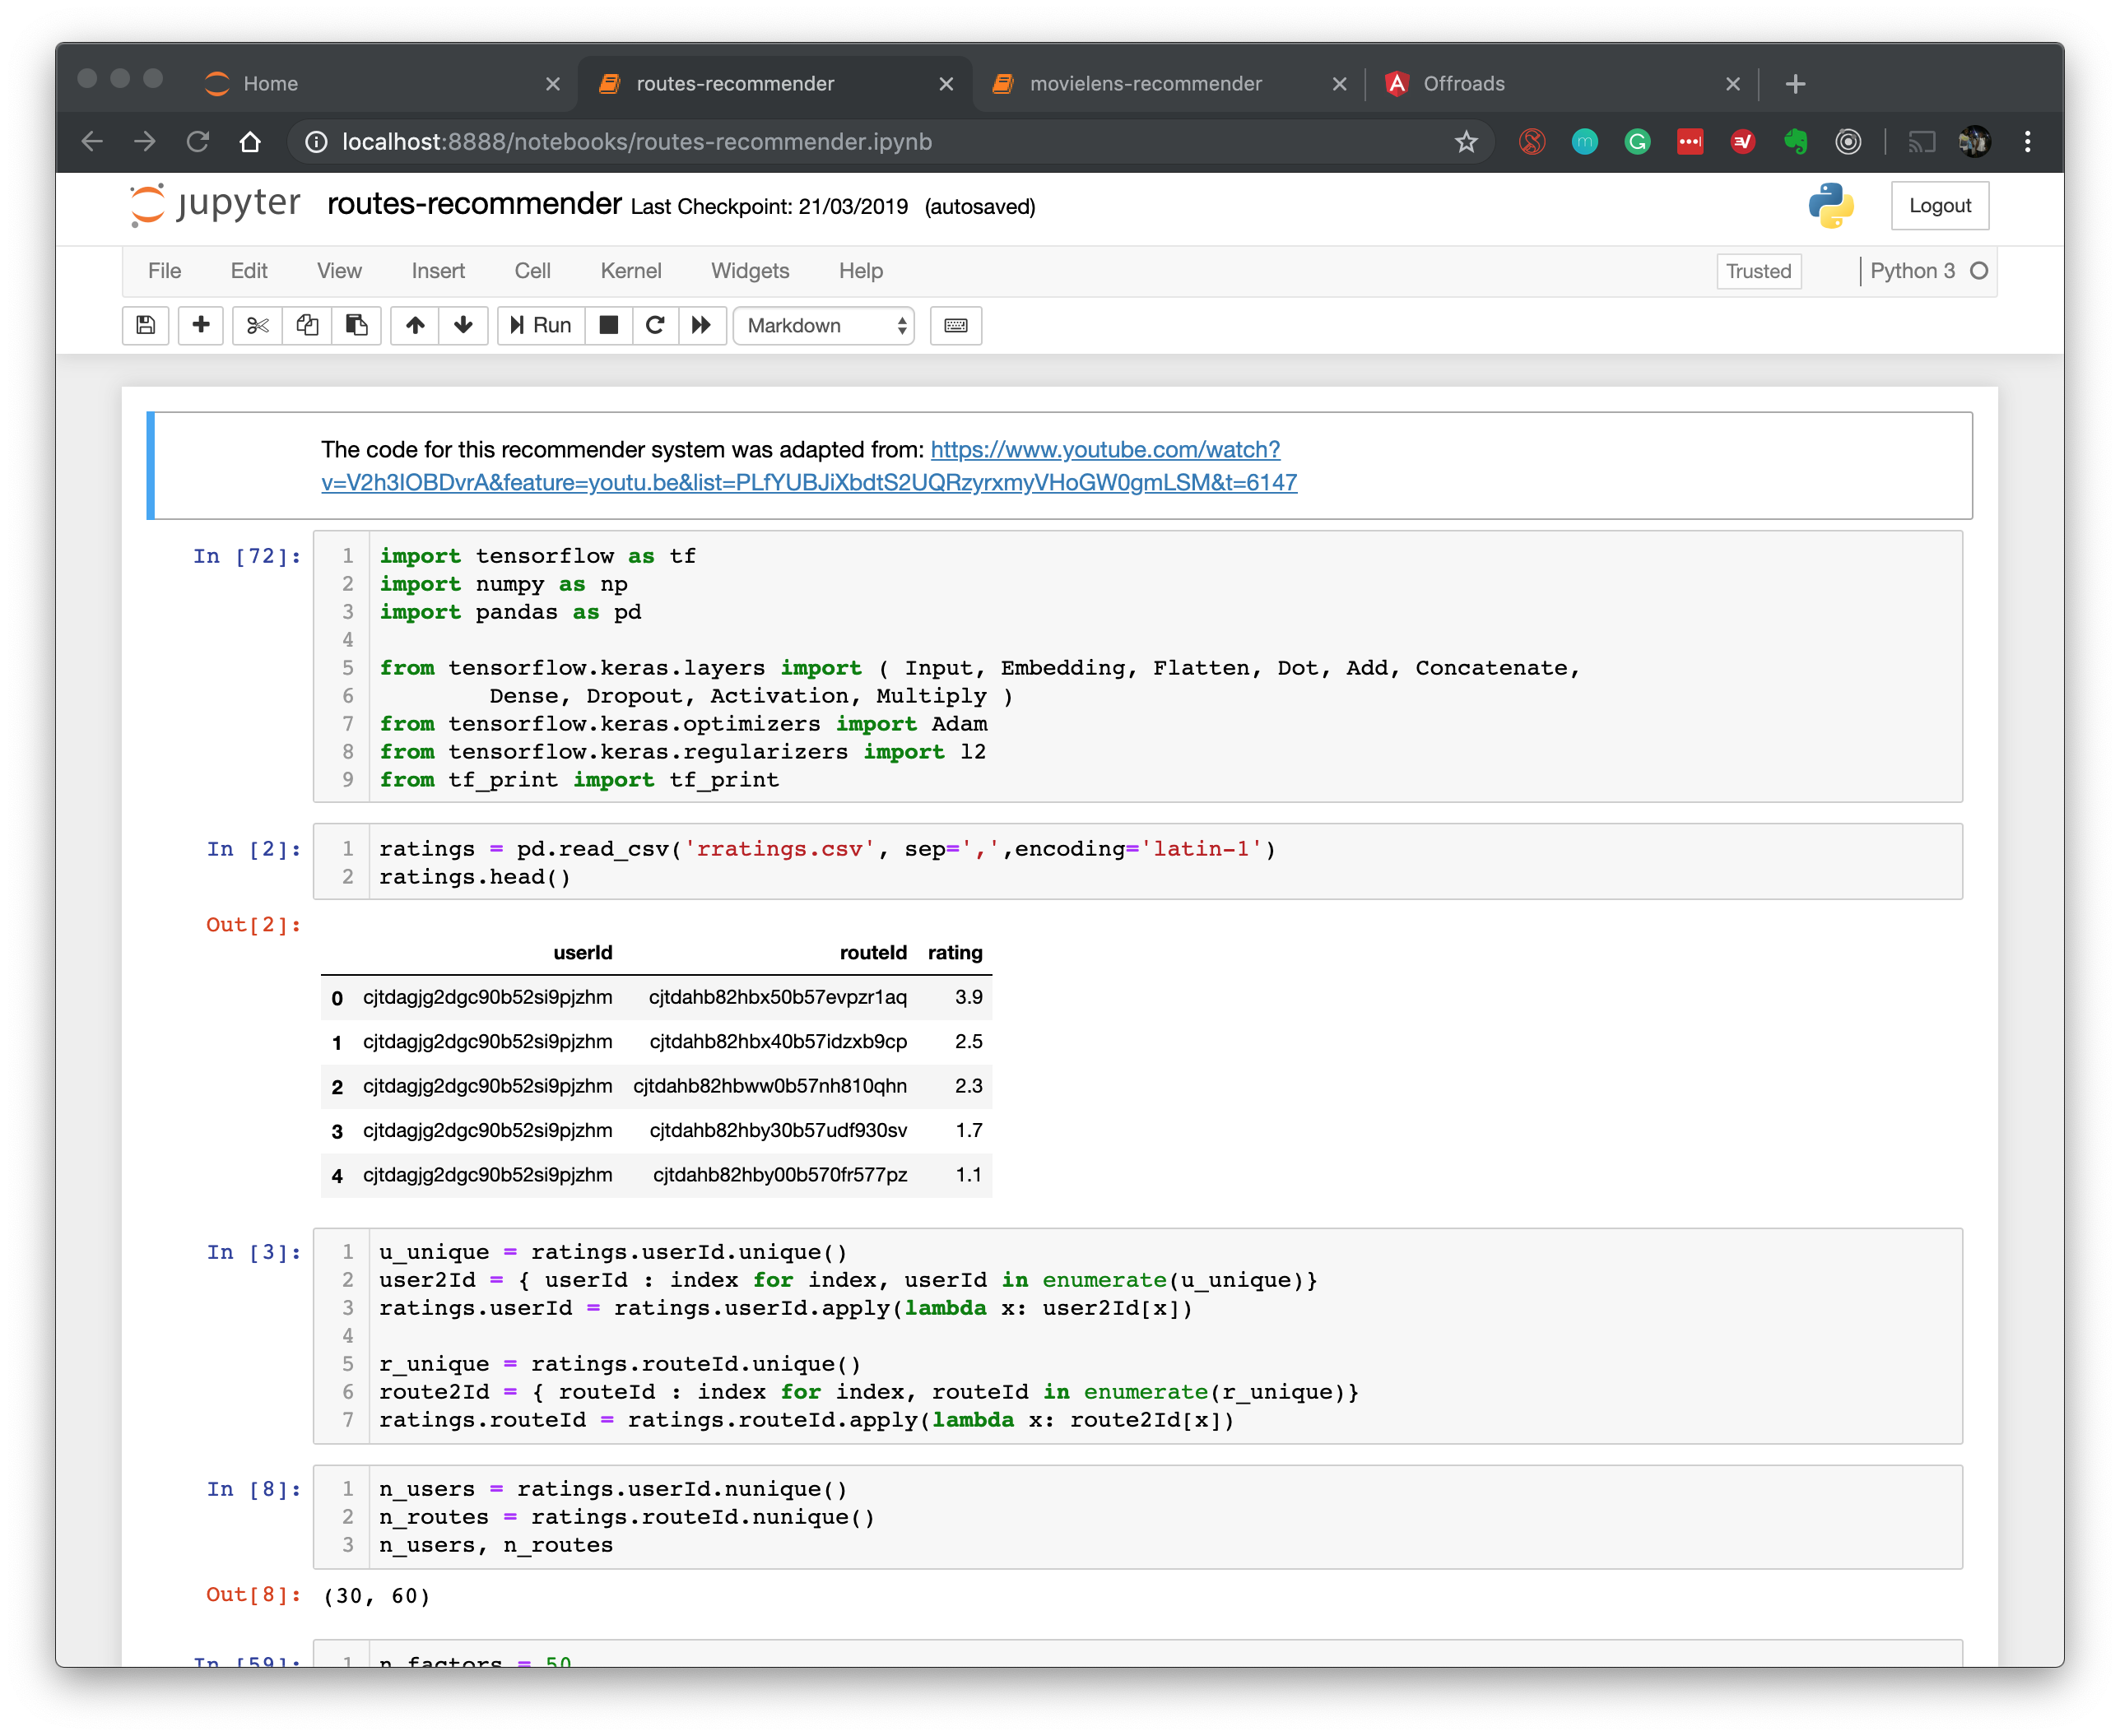
\includegraphics[width=\textwidth]{jupyter-notebook.png}
    \caption{Jupyter Notebook}
    \label{fig:JupyterNotebook}
\end{figure}


\chapter{Evaluation and Testing}
It is important to test the system. Not only manually testing the website, but also empirically testing the efficient of the Recommender system. One of the main problems that we have is that we do not have an original dataset to test our system, we discuss ways of overcoming this issue in section \ref{coldStartProble}.
\section{Quality of Recommender systems}
\subsection{Evaluation Metrics} \label{subsec:evaluationMetrics}
The quality of Recommender systems can evaluated using a variety of different empirical metrics \cite{isinkaye2015recommendation}. We use empirical methods because it gives us a statistical value we can aim to improve. It also gives us a value we can compare against other Recommender systems, allowing us to measure against industry standards and benchmarks
\subsection{Extreme Cold Start Problem} \label{coldStartProble}
To test our machine learning model, we would need to have training data to train our model on and then calculate the \acrshort{mse} to know how accurate our model is. However, as this is a completely new system, there is no previous data-set to train the machine learning model on which means that there is no way to test the model. One of the way's to solve this problem is to generate our own data-set.

\subsubsection{Generating Data-set}
Although this will not be an accurate data-set to train our model on, it would help test how good the machine learning model we created is. For the data-set we to need to generate users and routes. For each user and route, we assign 4 attributes: Terrain, Distance, Elevation and Scenery (representing four attributes of a route). For each user, we generate values for these attributes that will correspond with how much each user likes that attribute for a route as shown in table \ref{tab:genUserDataset}. 

The attribute values range from 0 to 9, 0 g extreme dislike and 9 meaning extreme like. Each route will also have values for this attributes which is how much of that attribute that the route has as shown in table \ref{tab:genRouteDataset}.

\begin{table}[ht]
    \centering
    \begin{tabular}{|c|c|c|c|c|}
        \hline
         User ID & Terrain & Distance & Elevation & Scenery  \\
         \hline
         \hline
         0 & 3 & 1 & 3 & 7  \\
         1 & 7 & 8 & 1 & 2 \\
         2 & 8 & 0 & 5 & 2 \\
         4 & 6 & 7 & 7 & 2 \\
         \hline
    \end{tabular}
    \caption{Example of User Data to help generate data-set}
    \label{tab:genUserDataset}
\end{table}

\begin{table}[ht]
    \centering
    \begin{tabular}{|c|c|c|c|c|}
        \hline
         Route ID & Terrain & Distance & Elevation & Scenery  \\
         \hline
         \hline
         0 & 5 & 1 & 3 & 7  \\
         1 & 7 & 5 & 1 & 2 \\
         2 & 8 & 0 & 5 & 8 \\
         4 & 6 & 7 & 7 & 9 \\
         \hline
    \end{tabular}
    \caption{Example of Route Data to help generate data-set}
    \label{tab:genRouteDataset}
\end{table}

We generate 30 users with 5 each from the sub classes in table \ref{tab:attributeSubClasses}. The sub classes are an attempt to represent different types of users and the attribute values are to reflect what they look for int trails. We also generate 60 routes with 10 from each of the sub classes in table \ref{tab:attributeSubClasses}.
\begin{table}[ht]
    \centering
    \begin{tabular}{|c|c|c|c|c|}
        \hline
         Sub-classes & Terrain & Distance & Elevation & Scenery \\
         \hline
         Hardcore & 7 - 9 & 7 - 9 & 7 - 9 & 0 - 9 \\  
         \hline
         Distance & 0 - 3 & 7 - 9 & 0 - 3 & 0 - 3 \\
         \hline
         Visual & 0 - 3 & 0 - 3 & 0 - 3 & 7 - 9 \\
         \hline
         Mountain & 0 - 3 & 0 - 3 & 7 - 9 & 0 - 3 \\
         \hline
         Casual & 0 - 3 & 0 - 3 & 0 - 3 & 0 - 3 \\
         \hline
         Random & 0 - 9 & 0 - 9 & 0 - 9 & 0 - 9 \\
         \hline
    \end{tabular}
    \caption{Caption}
    \label{tab:attributeSubClasses}
\end{table}

Each user runs and rates between 10 and 23 random routes from the generated routes. For each user and the route they run we calculate a \textit{like} value using the attribute values from the user and the route using equation \ref{eqn:Likes}. We then add another probability value that is created using a Gaussian Probability Distribution\cite{simon2007probability} to create and equal probability distribution. This probability value is to add a little bit of randomness to the like value. This represents if for example it was raining when a user runs a route which can affect how they feel about the route compared to normal conditions.

We then use this like value to calculate the rating by using the equation \ref{eqn:RatingCalculation}. We use the Sigmoid function\cite{wiki:SigmoidFunction}, which is a non-linear function\footnote{It's normally used as an activation function in neural networks}, that can map the calculated like value to a value between 0 - 1.

\begin{equation} \label{eqn:Likes}
    \textrm{likes} = \Bigg(\sum_{i=1}^{n=4}abs({u_i}-{r_i})\Bigg) + {p_i}
\end{equation}

\begin{equation} \label{eqn:RatingCalculation}
    \textrm{rating} = \big(\sigma(\textrm{likes}) \times 4\big) + 1
\end{equation}

We then use these generated ratings to help train our machine learning model. With tensor flow we can get our final \acrshort{mse} and root it to get our \acrfull{rmse}, the standard for comparing how good the Recommender system machine learning models are.

\subsection{Movie Lens Data-set}
Another way to test the system is to use an already existing data-set. One of the benefits of Recommender systems is that it can be applied to any generic user-item ratings matrix. Hence although we may not be able to find an already existing user-route ratings matrix, we can use another user-item ratings matrix to test it.

The dataset that I used is a popular dataset of user-movies ratings called the Movie lens Dataset\footnote{https://grouplens.org/datasets/movielens/}. The best thing about using this data set is that there are other online recommender systems that have been tested on this dataset that we can compare our \acrshort{rmse} score against\footnote{https://www.kaggle.com/learn/overview}\footnote{https://www.librec.net/release/v1.3/example.html}.

Create another model that is trained on our movie lens dataset based on the exact same code as the one for our original neural network model.

\section{Manual Testing}

\subsection{GraphQL Dev Tools}
It is important to be able to test the GraphQL queries before exposing them to the front-end. One of the benefits with GraphQL is the development tools it provides. This tools allows you to view the GraphQL schema you've defined, including all the possible operations available. It also allows you to test each operation.
\begin{figure}[ht]
    \centering
    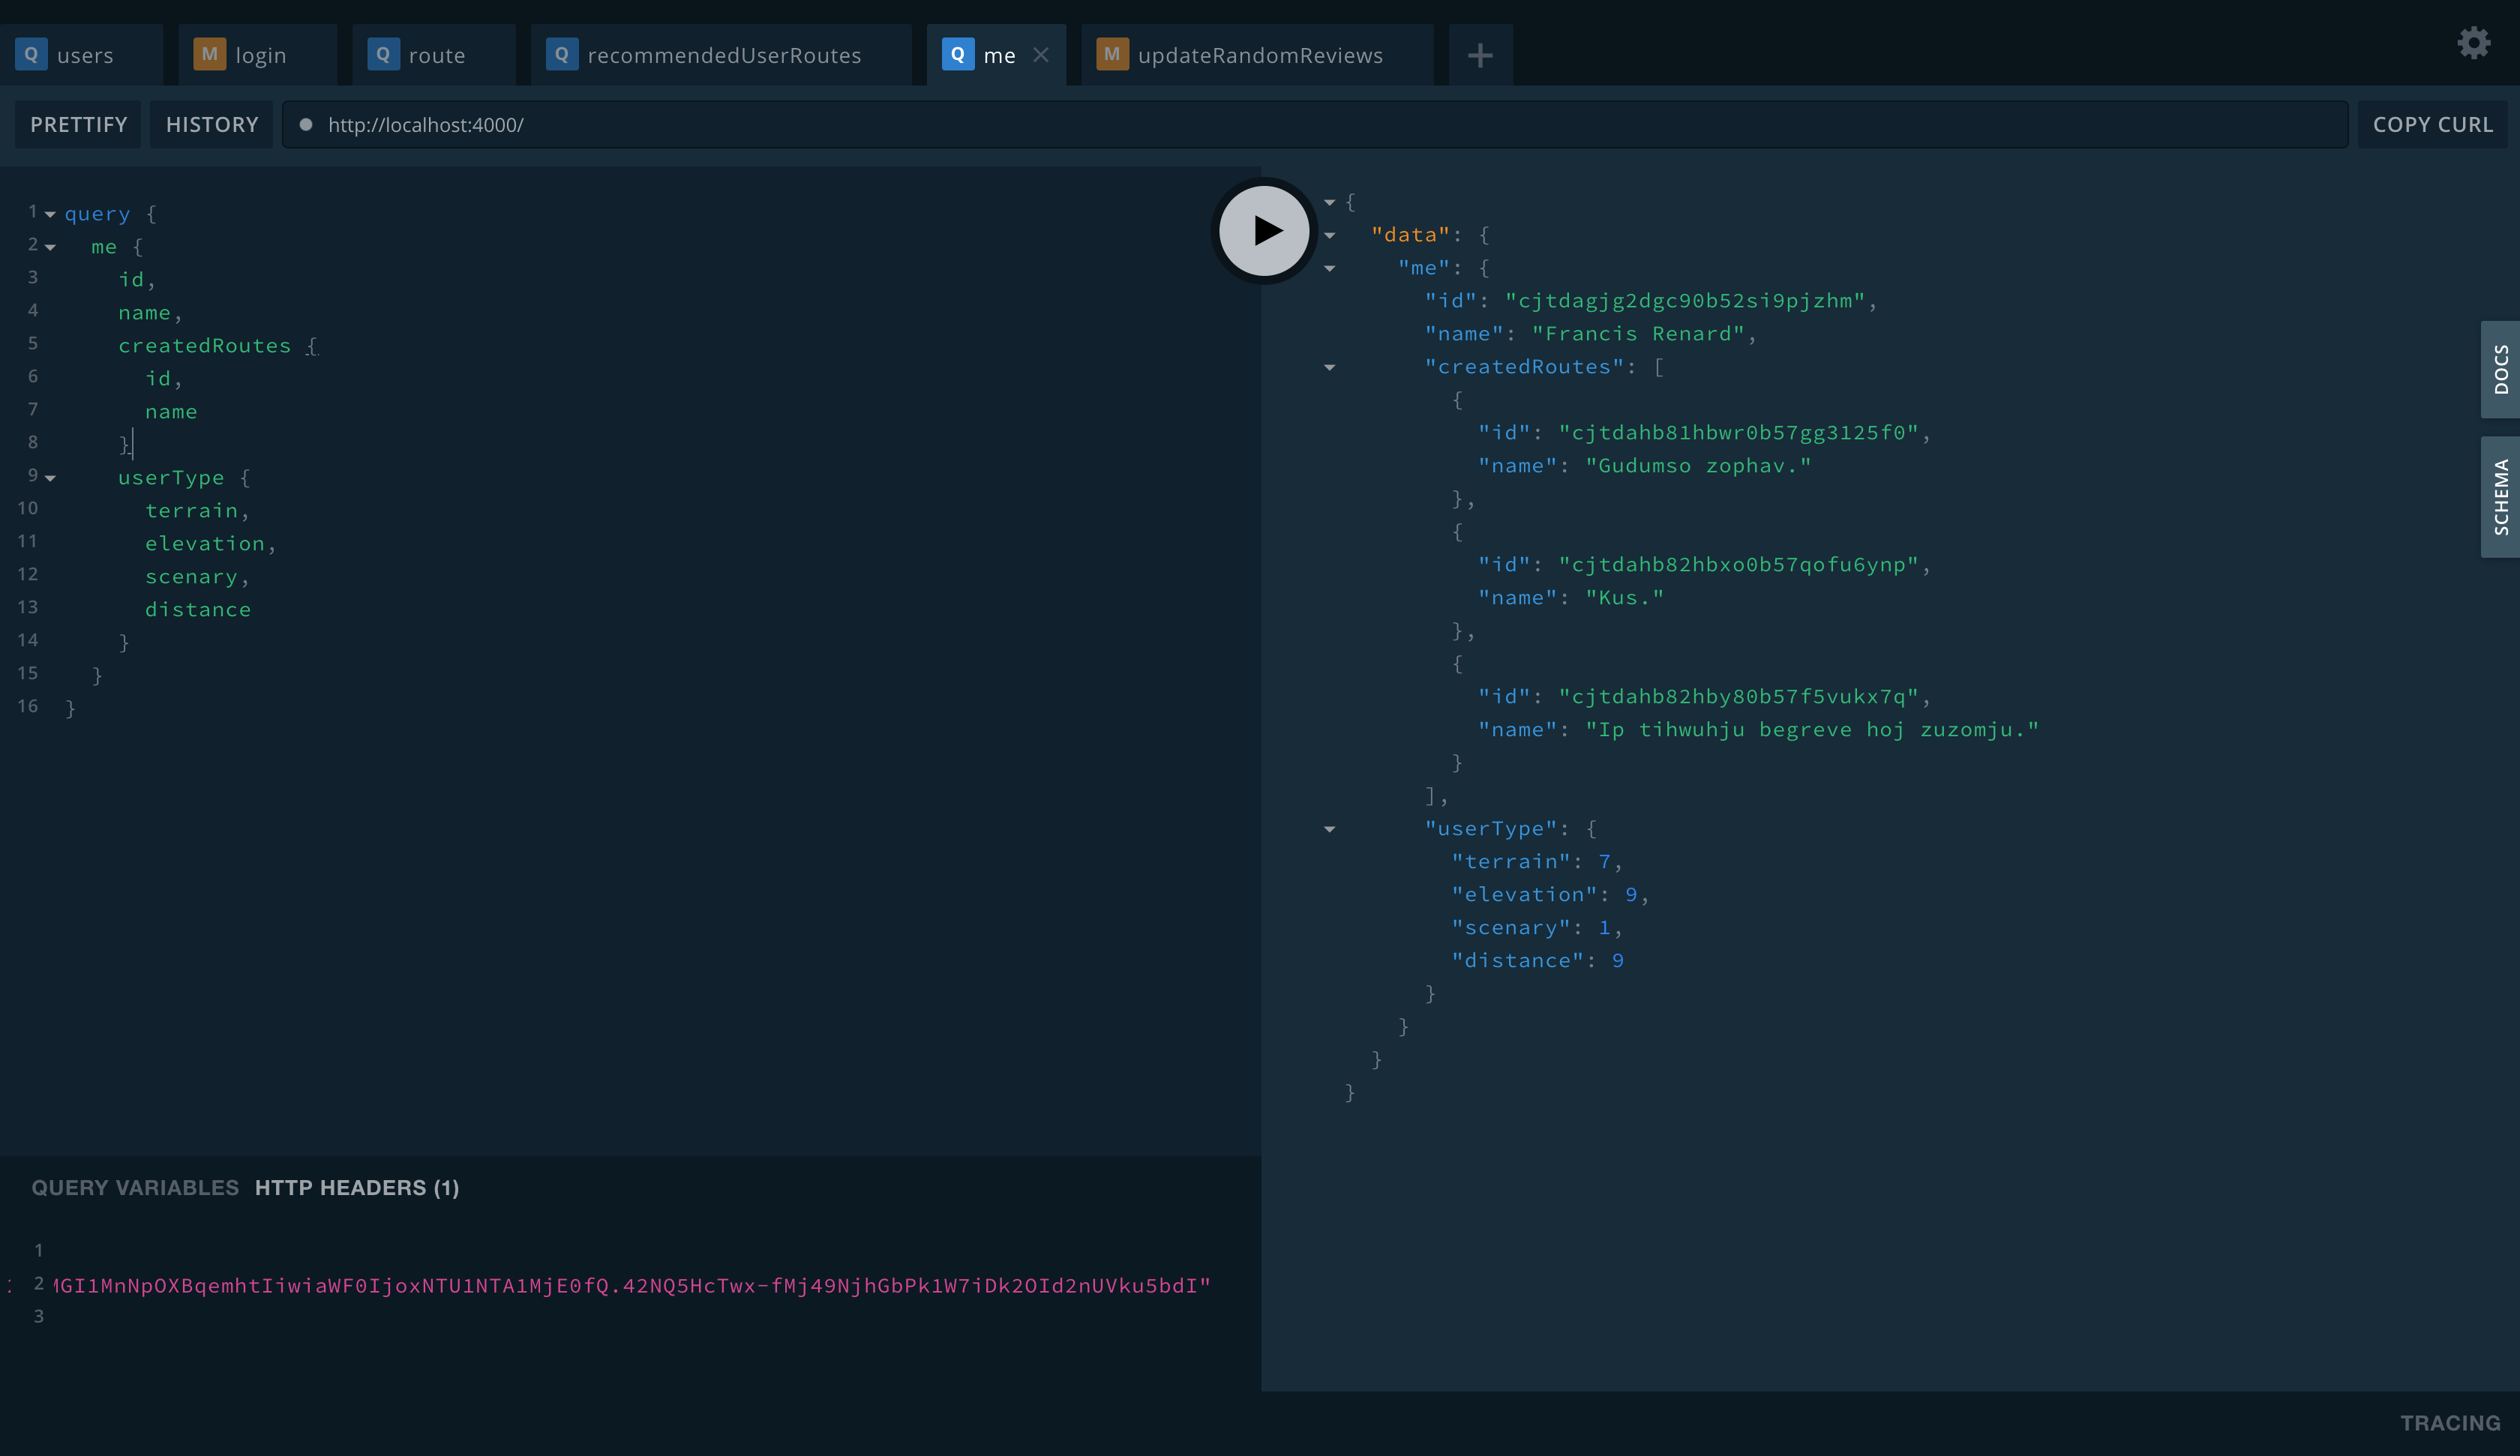
\includegraphics[width=0.75\textwidth]{graphql-dev.png}
    \caption{GraphQl Development Tools}
    \label{fig:graphQLDevTools}
\end{figure}

\subsection{Redux Dev Tools}
NgRx comes with dev tools as shown in figure \ref{fig:reduxDevTools}. It allows us to track the state of our application as it evolves from initial log-in, to router navigation and trail changes. This tool can be used to traverse the state of our application as it evolves. It allows us to ensure that the right actions are being called at the right times
\begin{figure}[ht]
    \centering
    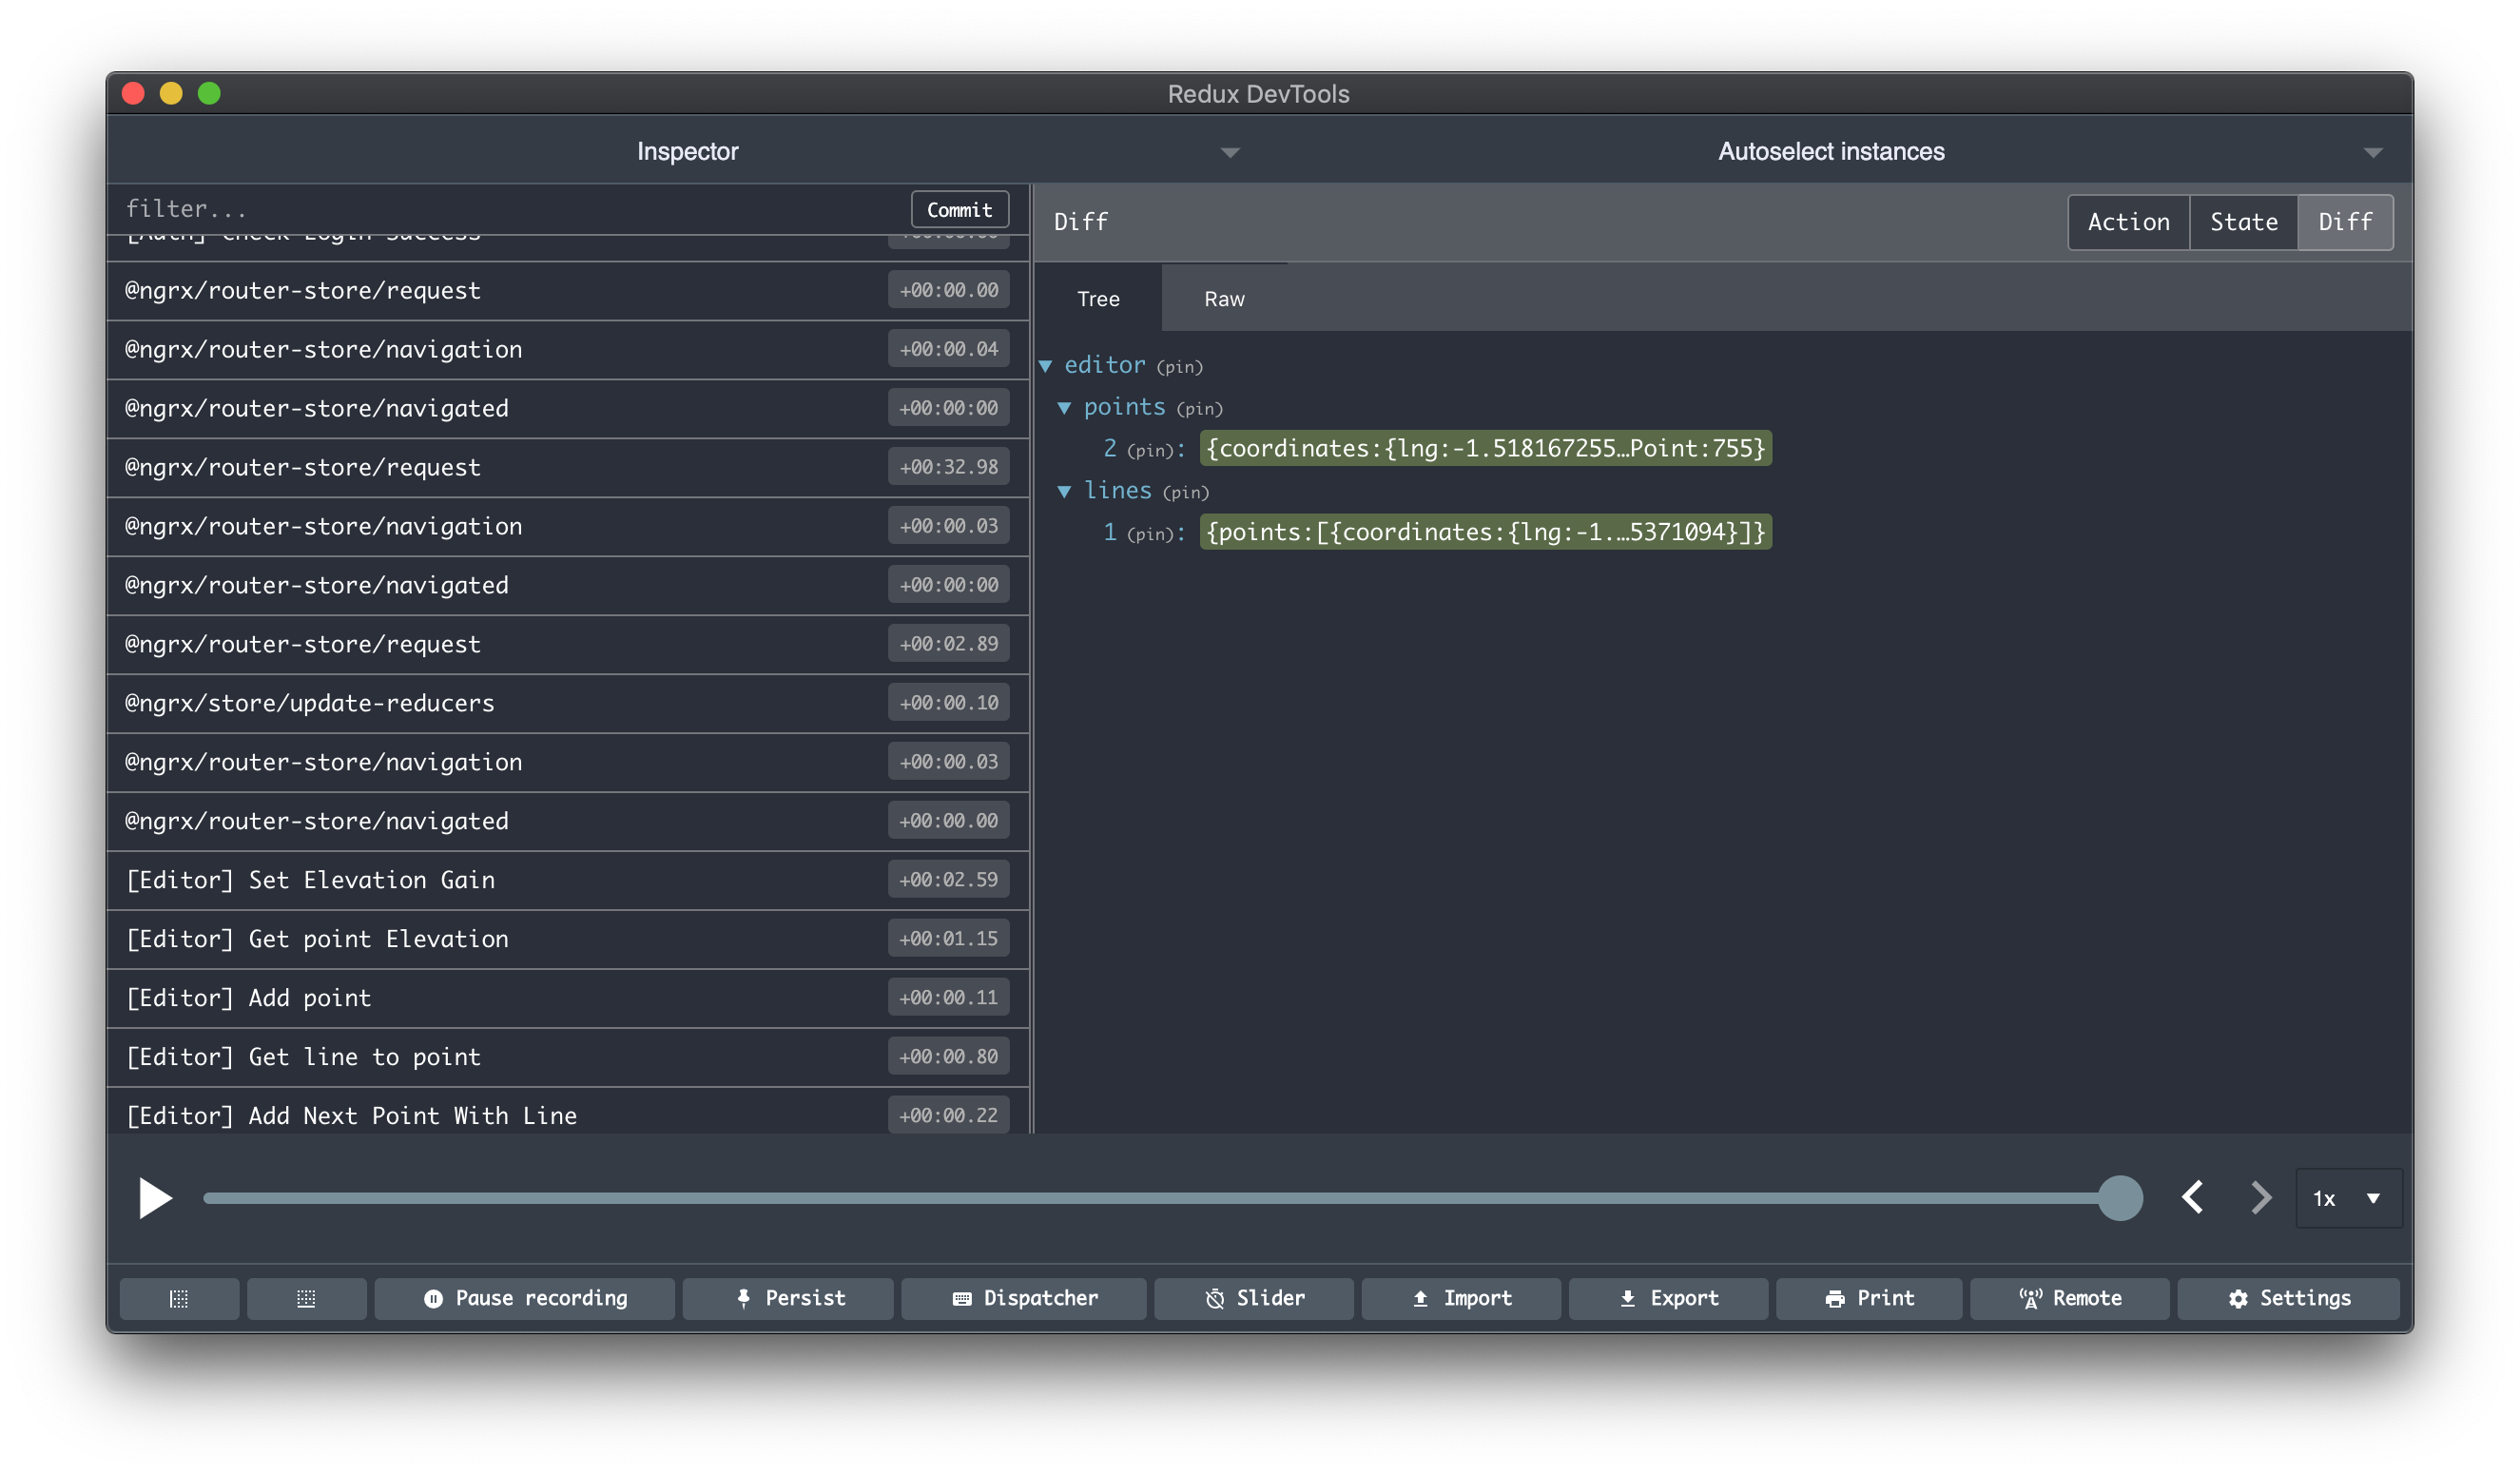
\includegraphics[width=0.75\textwidth]{redux-dev-tools.png}
    \caption{Redux Dev Tools}
    \label{fig:reduxDevTools}
\end{figure}


\section{Unit and Integration Testing}
To test the front-end we follow a standard industry methods of creating both unit tests and integration tests. Angular comes built with the Jasmine Testing framework, a JavaScript behaviour driven framework. Jasmine also use Karma, that allows us to run the tests on the browser.

Angular also provides Protractor for end to end testing on the front end
\chapter{Reflections}
\section{Planning and Management}
The project was split into 2 main action areas
\begin{itemize}
    \item The first part was to create the infrastructure of the website. This includes the frontend, backend and the trail interface discussed in the sections above.
    \item The second part was the creation of the recommender system. Including the research into the types of recommender systems that I could use and the technologies.
\end{itemize}

However one of the main problems with this is I greatly underestimated how hard it was building the infrastructure of the website. One of the major factors that slowed me down is learning GraphQL. It is a new technology that I'm not familiar with which made progress with it slow. And as it is quite new, and not used by many, there was no such community to get help from and no real documentation provided to use. 

This meant I was not able to focus alot on researching the recommender system's and could not use Content-based filtering and hybrid recommender systems to improve my overall recommender system.
\section{Future Work}
\subsection{Hybrid Recommender Systems}
One of the problem's we had with this system is there was no extra meta-data on the data for routes given. This prevented us from using content-based filtering. Now although collaborative filtering is a better recommender system than content-based filtering, a much better method would be combining the results from both systems. A hybrid recommender system would be useful to combine and rank the results from both of them to provide between suggestions.

\subsection{Exploring on a Map View}
One of the features that the other trail running websites provide as shown is \autoref{sec:TrailRunningApplications} is presenting the trails on a map view, that show's the location of each trail. This presents a more user friendly way of viewing the trails and also provides extra information of the location of where the trails are.

\subsection{Deploying the Website}
An important part of building any application is the method of deployment. I would have used one of the many online cloud services, preferably Amazon Web Services (AWS), to deploy the website. One of the mahor things of using this is that it allow's you to easily build scalable web applications. They also take away the complexity of dealing with hard ware issues. And it would provide extra resources needed, for example, machine learning specific architecture to improve the machine learning process.

\subsection{CI \& CD pipelines}
During development, I used alot of development tools. One strategy I could use to make both debugging and deployment easy is to use Continous Integration and Continous Deployment. This is very important for improving real life applications as it eleviates the problems that come with testing by adding automated testing and ensuring the main version of the application is not broken. It also simplifies the deployment of applications

\subsection{Mobile Application}
One of the problems with building a website solution is that it's not a very mobile solution. It's not easy to allow users to live record a trail as they run it, or their live data as they run an already ran trail to help in comparison. 

A better way for deliver this solution is to use a mobile application. However with a mobile application there's also the problem of developing for multiple Operating Systems, namely IOS and Android.

So we could use a hybrid framework to develop for both of these interfaces. I believe this would be a better solution than just developing a responsive website as it would have a more native feel. And it would have the benefit of not having to develop and maintain different projects for the same application.
\chapter{Conclusion}
In conclusion, the project covers a wide breadth of topic areas in the approach taking to solving the problems highlighted in \autoref{chap:Intro}. The project is aimed at trail runners who need a platform to be able to create, share and discover trails.

The interface discussed in \autoref{chap:TrailInterface} explains how we provide a well informative interface allowing users to create this interface. The map provider used is industry standard and sufficient research and comparisons was done to to come to this decision.

By examining the strengths and weaknesses of different techniques to creating a Recommender system, the project not only justifies the Recommender system approach with a detailed explanation on the benefits of the techniques used but also delivers a system that is able to compete with other proposed solutions. 

Thee project includes a full stack development process, bearing the results of all parts of the project in the form of a very presentable, polished and feature rich dynamic web application.

Finally, many parts of the project where evaluated to ensure that the systems where working efficiently. This included use of manual testing from clever development tools, industry testing using standing test approach methods and statistical analysis from empirical evaluation metrics. 

Overall, I believe that the project explores many research areas and produces a deliverable that has been well executed, well-evaluated and that I am proud of.

\printbibliography[heading=bibintoc]

\begin{appendices}
    \chapter{Mapping data returned} \label{appendix:mapDataReturned}

\section*{Mapbox Directions Result} \label{appSec:mapboxDirections}
\inputminted[frame=lines,framesep=2mm,baselinestretch=1.2,fontsize=\footnotesize]{json}{listings/mapbox-directions.json}
\captionof{listing}{Example of Directions returned from mapbox directions API}

\section*{Google Maps Elevation Results} \label{appSec:googleElevation}
\inputminted[frame=lines,framesep=2mm,baselinestretch=1.2,fontsize=\footnotesize]{json}{listings/google-elevation.json}
\captionof{listing}{Example of Google's elevation service data returned}
    \chapter{Server GraphQL Schema} \label{app:graphqlSchema}
\end{appendices}
\end{document}
